% -----------------------------------------  
% Autogenerated LaTeX file from XML DocBook  
% -----------------------------------------  
%%<params>
%% latex.encoding utf8
%%</params>
\documentclass{report}
\IfFileExists{ifxetex.sty}{%
    \usepackage{ifxetex}%
  }{%
    \newif\ifxetex
    \xetexfalse
  }
  \ifxetex
\usepackage{fontspec}
\usepackage{xltxtra}
\setmainfont{DejaVu Serif}
\setsansfont{DejaVu Sans}
\setmonofont{DejaVu Sans Mono}
\else
\usepackage[T2A,T2D,T1]{fontenc}
\usepackage{ucs}
\usepackage[utf8x]{inputenc}
\def\hyperparamadd{unicode=true}
\fi
\usepackage{fancybox}
\usepackage{makeidx}
\def\hyperparam{colorlinks,linkcolor=blue}
\def\DBKpublisher{\includegraphics{dblatex}}
\usepackage[french]{babel}
\usepackage{cmap}
\usepackage[hyperlink]{asciidoc-dblatex}
\lstset{inputencoding=utf8x, extendedchars=true}
\setuplocale{fr}
\setupbabel{fr}
\renewcommand{\DBKreleaseinfo}{}
\renewcommand{\DBKrevhistory}{}
\setcounter{tocdepth}{0}
\setcounter{secnumdepth}{1}
\renewcommand{\DBKdate}{29/12/2012}
\title{Introduction à SysML}
\author{Jean-{}Michel Bruel}
\hypersetup{%
pdfcreator={DBLaTeX-0.3.4},%
pdftitle={Introduction à SysML},%
pdfauthor={Jean-{}Michel Bruel}%
}
\renewcommand{\DBKindexation}{}
\makeindex
\makeglossary
\begin{document}
\lstsetup
\frontmatter
\maketitle
\tableofcontents
\listoffigures
\listoftables
\setcounter{secnumdepth}{-1}
\addtocontents{toc}{\protect\setcounter{tocdepth}{-1}\ignorespaces}
\setcounter{tocdepth}{-1}

\chapter{Remerciements}
\label{_remerciements}\hyperlabel{_remerciements}%

À faire au dernier moment…
\setcounter{secnumdepth}{1}
\addtocontents{toc}{\protect\setcounter{tocdepth}{0}\ignorespaces}
\setcounter{tocdepth}{0}
\setcounter{secnumdepth}{-1}
\addtocontents{toc}{\protect\setcounter{tocdepth}{-1}\ignorespaces}
\setcounter{tocdepth}{-1}

\chapter{Préface}
\label{_préface}\hyperlabel{_préface}%

Exemple de préface…
\setcounter{secnumdepth}{1}
\addtocontents{toc}{\protect\setcounter{tocdepth}{0}\ignorespaces}
\setcounter{tocdepth}{0}
\mainmatter
%
% PART
%

\part{Partie 1 : Introduction}
\label{_partie_1_introduction}\hyperlabel{_partie_1_introduction}%

% ------- 
% Chapter 
% ------- 

\chapter{Avant-{}propos}
\label{_avant_propos}\hyperlabel{_avant_propos}%

\section{Sur ce document}
\label{_sur_ce_document}\hyperlabel{_sur_ce_document}%

\subsection{A qui est destiné ce document?}
\label{_a_qui_est_destiné_ce_document}\hyperlabel{_a_qui_est_destiné_ce_document}%

Les étudiants qui découvrent le langage, mes collègues enseignants qui cherchent un document de support à leur cours et d’exercice accessible, et … moi-{}même (pour organiser mes notes diverses)!

\subsection{A qui n’est-{}il pas destiné?}
\label{_a_qui_n_8217_est_il_pas_destiné}\hyperlabel{_a_qui_n_8217_est_il_pas_destiné}%

Si vous appartenez à l’une de ces catégories, ce livre \textbf{n’est pas pour vous} :
\begin{itemize}

\item{} vous cherchez un livre de référence (pour cela, même s’il est en anglais, je conseille \hyperlink{FMS}{[FMS]})



\item{} vous voulez vous perfectionner (ce livre n’est qu’une introduction)



\item{} vous souhaitez préparer la certification de l’\href{http://www.omg.org}{OMG}\index{OMG} (mieux vaut vous plonger dans la spécification \hyperlink{SysML}{[SysML]})


\end{itemize}

\subsection{Historique}
\label{_historique}\hyperlabel{_historique}%

Ce document est la compilation de plusieurs années d’enseignement de \href{http://www.omgwiki.org/OMGSysML/}{SysML}\index{SysML} depuis 2007, que ce soit :
\begin{itemize}

\item{} au \href{http://dep-informatique.univ-pau.fr/live/masterTI}{Master TI}, de l’\href{http://www.univ-pau.fr/}{Université de Pau et des Pays de l’Adour} (cours d’introduction avec mon collègue et ami Nicolas Belloir),



\item{} au \href{http://spiderman-2.laas.fr/M2R-SAID/}{Master Recherche SAID}, de l’\href{http://www.univ-tlse3.fr}{UPS} (introduction),



\item{} au \href{http://mathsinfo.univ-tlse2.fr/accueil/formations/master-ice/}{Master ICE} de l’\href{http://www.univ-tlse2.fr}{Université de Toulouse II -{} Le Mirail} (introduction avec mon collègue et ami Pierre de Saqui Sannes),



\item{} au \emph{Master of Science} de Göteborg, Suède (introduction réalisée par Nicolas Belloir),



\item{} à l’\href{http://www.uag.mx/}{Universitad Autónoma de Guadalajara}, au Mexique (40h de formation professionnelle aux employés de Continental),



\item{} ou plus récemment au \href{http://www.dept-info.ups-tlse.fr/index.php?option=com_content&view=article&id=294&Itemid=697&lang=fr}{Master DL-{}SI} de l’\href{http://www.univ-tlse3.fr}{UPS}.


\end{itemize}

Vous trouverez en référence (cf. \hyperlink{refs}{Bibiliographie}) les ouvrages et autres documents utilisés.

\section{Sur l’auteur}
\label{_sur_l_8217_auteur}\hyperlabel{_sur_l_8217_auteur}%
\begin{itemize}

\item{} Professeur à l’\href{http://www.univ-toulouse.fr}{Univesité de Toulouse} 


\item{} Co-{}fondateur de l’association \href{http://www.sysml-france.fr}{SysML-{}France}\index{SysML-{}France} en 2009



\item{} Membre du comité éditorial de la revue \emph{\href{http://www.sosym.org}{Software and System Modeling journal}} depuis sa création en 2002



\item{} Membre du \emph{Steering Committee} de la conférence ACM/IEEE \href{http://www.modelsconference.org/}{MODELS} depuis 2008



\item{} Enseignant en modélisation depuis 1995



\item{} Marié, une (merveilleuse) fille


\end{itemize}

\section{Comment lire ce document?}
\label{comment-lire}\hyperlabel{comment-lire}%

\subsection{Version électronique}
\label{_version_électronique}\hyperlabel{_version_électronique}%

Ce document a été réalisé de manière à être lu de préférence
dans sa version électronique, ce qui permet de
naviguer entre les références et les renvois interactivement, de consulter
directement les documents référencés par une URL, etc.
\begin{DBKadmonition}{images/icons/note.png}{Note}

Si vous lisez la version papier de ce document, ces liens clickables ne
vous servent à rien, mais n’hésitez pas à en consulter la version \href{http://www.sysML.fr}{électronique}!
\end{DBKadmonition}

\subsection{Conventions typographiques}
\label{_conventions_typographiques}\hyperlabel{_conventions_typographiques}%

J’ai utilisé un certain nombre de conventions personnelles
pour rendre ce document le plus agréable à lire et le plus
utile possible, grâce notamment à la puissance d’\href{http://www.methods.co.nz/asciidoc}{AsciiDoc}\index{AsciiDoc} :
\begin{itemize}

\item{} des mises en formes particulières (e.g., \texttt{Nom\penalty5000 D\penalty5000 e\penalty5000 B\penalty5000 loc} pour un élément de modèle),



\item{} des références bibliographiques, présentées en fin de document
(cf. \hyperlink{refs}{Bibliographie}),



\item{} tous les \emph{flottants} (figures, tableaux) sont
listés à la suite de la table des matière,



\item{} les termes anglais (souvent incontournables) sont repérés
en \emph{italique}, non pas pour indiquer qu’il s’agit d’un
mot anglais, mais pour indiquer au lecteur que nous employons
volontairement ces termes (e.g., \emph{Requirements}).


\end{itemize}

Les figures, sauf mention contraire, ont été réalisées avec l’outil \href{http://www.topcased.org}{TOPCASED}\index{Topcased} en français.
Le titre des figures indique (entre parenthèses) un \texttt{R} pour les figures issues de \href{http://www-142.ibm.com/software/products/us/en/ratirhap}{Rhapsody}\index{Rhapsody} et un \texttt{UK} pour les figures en anglais. Les conventions (de nommage notamment) sont regroupées en section Chapitre \ref{conventions}.
\begin{DBKadmonition}{images/icons/important.png}{Pourquoi parler de "document"?}

Parce que j’ignore la version que vous êtes en train de lire. A partir de l’\href{main.txt}{original}, plusieurs versions ont été générées grâce à \href{http://www.methods.co.nz/asciidoc}{AsciiDoc}\index{AsciiDoc}:
\begin{itemize}

\item{} pour le web (Moodle) au format \href{http://www.sysml.fr/main}{html} 


\item{} pour présentation (en amphi par exemple) au format \href{http://www.sysml.fr/slidy}{slidy} ou \href{http://www.sysml.fr/deckjs}{deck.js} 


\item{} pour impression au format \href{http://www.sysml.fr/main.pdf}{pdf} (bien que bien sûr nous vous recommandons l’achat du livre)



\item{} pour lire au format \href{http://www.sysml.fr/main.mobi}{Kindle} (bientôt!)


\end{itemize}
\end{DBKadmonition}

\subsection{Utilisation et autres mentions légales}
\label{_utilisation_et_autres_mentions_légales}\hyperlabel{_utilisation_et_autres_mentions_légales}%


\begin{sidebar}

Dernière MAJ : 29/12/2012 -{} 10:17:50 CET\newline
 Document généré par \href{mailto:bruel@irit.fr}{Jean-{}Michel Bruel} via \href{http://www.methods.co.nz/asciidoc}{AsciiDoc}\index{AsciiDoc} (version \texttt{8.\penalty0 6.\penalty0 8}) de \emph{Stuart Rackham}.
La version présentation a été générée en utilisant \href{http://www.w3.org/Talks/Tools/Slidy2/}{W3C HTML Slidy} © de \emph{Dave Raggett}, amélioré par \href{mailto:jean-michel.inglebert@univ-tlse2.fr}{Jean-{}Michel Inglebert}.
Pour l’instant ce document est libre d’utilisation et géré par la \emph{Licence Creative Commons}.
\noindent\imgexists{images/88x31.png}{{\imgevalsize{images/88x31.png}{
\includegraphics[scale=0.3]{images/88x31.png}}}}{images/88x31.png} \href{http://creativecommons.org/licenses/by-sa/3.0/}{licence Creative Commons Paternité -{} Partage à l'Identique 3.0 non transposé}.
\end{sidebar}

N’hésitez pas à m’envoyer vos remarques en tout genre en m'écrivant à \href{mailto:bruel@irit.fr}{bruel@irit.fr}.

\section{Méthode pour cet ouvrage}
\label{_méthode_pour_cet_ouvrage}\hyperlabel{_méthode_pour_cet_ouvrage}%
\begin{quote}

Everything should be made as simple as possible, but not simpler.

\hspace*\fill--- Albert Einstein
\end{quote}

Mon approche pédagogique repose sur quelques principes, que j’ai essayé de mettre en oeuvre dans
cet ouvrage :

\noindent
\begin{description}
\item[{ La répétition
}] \hspace{0em}\\
         Par exemple certains diagrammes sont abordés plusieurs fois (comme le diagramme paramétrique). Le lecteur pourra avoir une impression de redite par moment. Sauf erreur de ma part (toujours possible!), c’est volontaire. En général les répétitions vont en niveau de précision, de détails et de complexité croissant. Ces répétitions sont limitées dans la version livre de cet ouvrage
(car toute longueur inutile a un coût dans ce cas).

\item[{ L’illustration
}] \hspace{0em}\\
         Dans la mesure du possible, j’essaye de donner des exemples aux principes énoncés. Vous trouverez donc plus d’exemples que de définitions.

\item[{ Le référencement
}] \hspace{0em}\\
         Les définitions ou autres affirmations sont tirées d’ouvrages de référence généralement citées.

\item[{ La "carte de base"
}] \hspace{0em}\\
         J’aime réaliser une "carte" \footnote{
voir aussi le concept de \emph{Mind Maps}.
} qui sert à "placer" les différents concepts abordés. Il me semble que cela permet aux étudiants de raccrocher les nouveaux concepts aux précédents.

\end{description}

Aucune connaissance particulière d’\href{http://www.uml.org/}{UML}\index{UML} n’est nécessaire, même si j’y fais référence à plusieurs endroits pour les étudiants qui connaissent cette notation (quasiment enseignée partout maintenant comme langage de modélisation).
Il s’agit d’un parti pris prenant en compte plusieurs points :
\begin{itemize}

\item{} La plupart des ingénieurs systèmes ne connaissent pas \href{http://www.uml.org/}{UML}\index{UML}.



\item{} Les étudiants de STI2D ne connaissent pas \href{http://www.uml.org/}{UML}\index{UML} et sont pourtant formés à \href{http://www.omgwiki.org/OMGSysML/}{SysML}\index{SysML}.



\item{} Ceux qui connaissent \href{http://www.uml.org/}{UML}\index{UML} auront sûrement plaisir à retrouver les bases.


\end{itemize}

% ------- 
% Chapter 
% ------- 

\chapter{C’est quoi SysML?}
\label{_c_8217_est_quoi_sysml}\hyperlabel{_c_8217_est_quoi_sysml}%

Si vous ne deviez lire qu’un seul chapitre, voilà ce qu’il faudrait retenir.

\section{Fiche d’identité}
\label{_fiche_d_8217_identité}\hyperlabel{_fiche_d_8217_identité}%


\begin{sidebar}
\begin{itemize}

\item{} Date de naissance non officielle : 2001!



\item{} Première spécification adoptée à l’\href{http://www.omg.org}{OMG}\index{OMG} : 19 septembre 2007



\item{} Version actuelle : \href{http://www.sysml.org/docs/specs/OMGSysML-v1.3-12-06-02.pdf}{1.3} (12/06/2012)



\item{} Paternité : \href{http://www.omg.org}{OMG}\index{OMG}/\href{http://www.uml.org/}{UML}\index{UML} + \href{http://www.incose.org/}{INCOSE}\index{INCOSE} 


\item{} Auteurs principaux :

\begin{itemize}

\item{} Conrad Bock



\item{} Cris Kobryn



\item{} Sanford Friedenthal


\end{itemize}

\end{itemize}
\end{sidebar}

\section{SysML, c’est…}
\label{_sysml_c_8217_est_8230}\hyperlabel{_sysml_c_8217_est_8230}%

\noindent
\begin{description}
\item[{ Un ensemble de 9 types de diagrammes
}] ~\begin{itemize}

\item{} Diagrammes structuraux

\begin{itemize}

\item{} Diagrammes de définition de blocs (\texttt{bdd})



\item{} Diagrammes internes de blocs (\texttt{ibd})



\item{} Diagrammes paramétriques (\texttt{par})



\item{} Diagrammes de packages (\texttt{pkg})


\end{itemize}


\item{} Diagrammes comportementaux

\begin{itemize}

\item{} Diagrammes de séquence (\texttt{seq})



\item{} Diagrammes d’activité (\texttt{act})



\item{} Diagrammes de cas d’utilisation (\texttt{uc})



\item{} Diagrammes d'états (\texttt{st})


\end{itemize}


\item{} Diagramme d’exigence (\texttt{req})


\end{itemize}
\item[{ Un profil \href{http://www.uml.org/}{UML}\index{UML} }] \hspace{0em}\\
         C’est à dire une \textbf{extension} de cette notation, un ensemble de nouveaux concepts et éléments qui sont définis à partir des éléments de base d’\href{http://www.uml.org/}{UML}\index{UML}. Un exemple : le \texttt{bloc} qui n’est qu’une redéfinition de la \texttt{cla\penalty5000 sse}.

\item[{ Une notation
}] \hspace{0em}\\
         Une notation de plus en plus enseignée et connue et qui servira donc de plus en plus de \textbf{référence} à la modélisation des systèmes.

\end{description}

\section{SysML, ce n’est pas…}
\label{_sysml_ce_n_8217_est_pas_8230}\hyperlabel{_sysml_ce_n_8217_est_pas_8230}%

\noindent
\begin{description}
\item[{ Une méthode
}] \hspace{0em}\\
         En effet, contrairement à ce que beaucoup pensent en l’abordant, \href{http://www.omgwiki.org/OMGSysML/}{SysML}\index{SysML} ne propose pas de démarche particulière de développement de système. C’est à la fois sa force (votre méthode existante pourra continuer à être utilisée) comme sa faiblesse car cette absence de guide méthodologique fait souvent défaut à son utilisation.

\item[{ Un outil
}] \hspace{0em}\\
         Nous verrons en effet que \href{http://www.omgwiki.org/OMGSysML/}{SysML}\index{SysML} ne fait que ce qu’on veut bien en faire. Comme tout langage il est limité dans son pouvoir d’expression, mais surtout il reste une simple notation qu’il convient d’utiliser avec des outils et des démarches associées.

\item[{ Un raton laveur
}] \hspace{0em}\\
         C’est juste pour voir ceux qui suivent.\index{Raton laveur} 
\end{description}

\section{Références et liens utiles}
\label{_références_et_liens_utiles}\hyperlabel{_références_et_liens_utiles}%

Vous trouverez en fin d’ouvrage un ensemble de liens utiles (cf. Chapitre \ref{liens}) et de références (cf. \hyperlink{refs}{bibliographie}).

% ------- 
% Chapter 
% ------- 

\chapter{A propos du Bac STI2D}
\label{STI2D}\hyperlabel{STI2D}%

Si vous utilisez cet ouvrage dans le cadre du bac STI2D \index{STI2D} (Sciences et Technologies de l’Industrie et du Développement Durable) qui a introduit depuis 2011 la notation \href{http://www.omgwiki.org/OMGSysML/}{SysML}\index{SysML} au programme, nous donnons
ici des conseils sur l’utilisation de ce cours \footnote{
Je remercie au passage les collègues de Lycée rencontrés dans le cadre de \href{http://www.sysml-france.fr}{SysML-{}France}\index{SysML-{}France} pour nos fructueuses discussions à ce sujet.
}.

L’objectif en STI2D \index{STI2D} n’est pas de former des spécialistes de \href{http://www.omgwiki.org/OMGSysML/}{SysML}\index{SysML} mais de permettre à tous d’apprendre une notation pour la modélisation de système qui se veut universelle. Il ne faut donc pas viser la complétude ou même demander trop de détails. La logique de la démarche de modélisation et l’importance de la communication devront primer.
\begin{DBKadmonition}{images/icons/note.png}{Note}

A l’heure où nous écrivons ces lignes, il est également prévu de l’enseigner en classe prépa dès 2013.
\end{DBKadmonition}

\section{Utilisation pratique}
\label{_utilisation_pratique}\hyperlabel{_utilisation_pratique}%

Cet ouvrage est tout à fait utilisable dans le cadre des cours dispensés en STI2D \index{STI2D}.
Seul un sous-{}ensemble des diagrammes de \href{http://www.omgwiki.org/OMGSysML/}{SysML}\index{SysML} a été retenu.
Les élèves et les enseignants du bac STI2D \index{STI2D} pourront trouver dans ce document des
éléments utiles sur ces diagrammes :
\begin{itemize}

\item{} diagramme des exigences (cf. Chapitre \ref{reqs})



\item{} diagramme des cas d’utilisation (cf. Section \ref{usecase})



\item{} diagramme de séquences (cf. Section \ref{seq})



\item{} diagramme d'états (cf. Section \ref{stm})



\item{} diagramme de définition de blocs (cf. Section \ref{bddsec})



\item{} diagramme de blocs internes (cf. Section \ref{ibd})


\end{itemize}

Ces 6 diagrammes sont tous traités dans cet ouvrage à un niveau qui devrait correspondre
à l’utilisation qui en est faite en STI2D \index{STI2D}.

Ces 6 diagrammes servent trois objectifs principaux inscrits au programme et dont les
élèves pourront également trouver des éléments de réflexion :
\begin{itemize}

\item{} Modélisation des exigences  (cf. Chapitre \ref{exigences})



\item{} Modélisation structurelle (cf. Chapitre \ref{structure})



\item{} Modélisation comportementale (cf. Chapitre \ref{comportement})


\end{itemize}

\section{Pour aller plus loin}
\label{_pour_aller_plus_loin}\hyperlabel{_pour_aller_plus_loin}%

Les questions et exercices de fin de chapitres de la partie notation seront peut-{}être d’un niveau plus avancé pour servir véritablement d’exercices, mais pourront amener  à une réflexion encadrée par l’enseignant.

Un blog récent recense les supports en liens avec STI2D \index{STI2D} : \href{http://www.scoop.it/t/formation-sysml-sti2d}{http://www.scoop.it/\-t/\-formation-{}sysml-{}sti2d}.

% ------- 
% Chapter 
% ------- 

\chapter{Un exemple fil rouge}
\label{_un_exemple_fil_rouge}\hyperlabel{_un_exemple_fil_rouge}%

L’exemple de système qui sera modélisé tout au long de ce livre en guise d’exemple
est l’exemple d’un système de gestion et de supervision de crise. Les détails sont
donnés en annexe (cf. \hyperlink{appendix}{Annexes}).

Il existe un certain nombre d’autres exemple complets :
\begin{itemize}

\item{} Le radio-{}réveil de \href{http://www.dotnetguru2.org/proques/index.php}{Pascal Roques} \hyperlink{Roques2010}{[Roques2010]}, un exemple simpliste mais didactique  qui a le mérite d'être déjà connu des modeleurs \href{http://www.uml.org/}{UML}\index{UML} qui ont lu ses livres.



\item{} Le distilleur de \hyperlink{FMS}{[FMS]}, un exemple très complet et lui aussi très connu car beaucoup utilisé dans les tutoriels issus de l’\href{http://www.omg.org}{OMG}\index{OMG}.



\item{} Le pacemaker de \hyperlink{SeeBook2012}{[SeeBook2012]}\footnote{
Nous avons réalisé le chapitre d’introduction à \href{http://www.omgwiki.org/OMGSysML/}{SysML}\index{SysML} de cet ouvrage.
}, un exemple très récent et dont l’avantage est d'être traité selon plusieurs approches différentes et complémentaires (\href{http://www.omgwiki.org/OMGSysML/}{SysML}\index{SysML}, \href{http://www.aadl.info/}{AADL} et \href{http://www.omgmarte.org/}{MARTE}\index{MARTE}).


\end{itemize}

Les exemples complets ont le mérite de donner une vue d’ensemble des liens qui peuvent exister entre les différents diagrammes. On peut y voir comment ces diagrammes sont complémentaires les uns des autres. Ils sont en général plus réalistes que les diagrammes utilisés pour illustrer tel ou tel concept de la notation.

\section{Enoncé}
\label{_enoncé}\hyperlabel{_enoncé}%
\begin{DBKadmonition}{images/icons/note.png}{Note}

Cette étude de cas est tirée de \href{http://www.springerlink.com/content/9028524720q17475/}{Kienzle2010}
\end{DBKadmonition}

Le système \textbf{CMS} (\emph{crash management system}) est un système distribué de gestion d’accidents
qui est responsable de la coordination et de la communication entre un coordinateur présent dans
une caserne de pompiers (appelé FSC pour \emph{Fire Station Coordinator}) et un autre présent dans un
poste de police (appelé PSC pour \emph{Police Station Coordinator}) afin de gérer une crise dans un
délai raisonnable.
\begin{figure}[H]

\begin{center}
\imgexists{images/CMS.png}{{\imgevalsize{images/CMS.png}{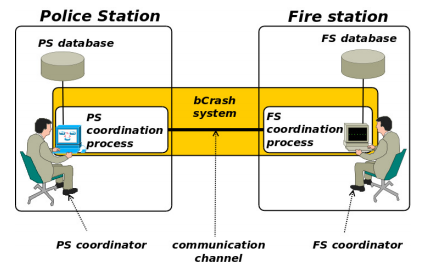
\includegraphics[scale=0.7]{images/CMS.png}}}}{images/CMS.png}
\end{center}
\caption{Le système CMS}
\end{figure}

La communication interne entre les membres de la police (y compris le PSC) est en dehors du
domaine qui nous intéresse ici (la gestion de crise). La même hypothèse s’applique aux
communications internes ou avec des acteurs externes côté pompiers (y compris le FSC).
Les informations concernant la crise ainsi que tout ce qui a trait aux tâches des coordinateurs
sont mises à jour et maintenues pendant et après la crise.

Il n’existe pas de base de données centrale; caserne de pompiers et police ayant leur
base de données respectives distinctes et seulement accessible aux autre à travers le
système CMS. Chaque processus de coordination est donc en charge de l’ajout et la mise
à jour des informations dans sa base de données respective.

CMS commence à fonctionner au moment où une crise donnée a été détectée et déclarée à la fois à la
caserne de pompiers et au poste de police.

Toutes les caractéristiques des différents acteurs sont détaillées ci-{}dessous.

\subsection{Coordinateur des pompiers (FSC)}
\label{_coordinateur_des_pompiers_fsc}\hyperlabel{_coordinateur_des_pompiers_fsc}%

Un FSC maintient le contrôle sur une situation de crise en communiquant avec le coordinateur du poste de police
(PSC) ainsi que les pompiers.

Pour atteindre ses objectifs, les responsabilités d’un FSC sont les suivantes :
\begin{itemize}

\item{} de déterminer où, quand et combien de camions de pompiers à envoyer,



\item{} de communiquer avec le PSC pour se présenter,



\item{} de garder le PSC informé en ce qui concerne la crise,



\item{} de proposer une stratégie pour traiter la crise,



\item{} parvenir à un accord avec le PSC sur la façon de procéder,



\item{} de recevoir des mises à jour concernant la crise côté pompiers, et



\item{} de rassembler et de diffuser des informations actualisées aux pompiers.


\end{itemize}

\subsection{Pompiers}
\label{_pompiers}\hyperlabel{_pompiers}%

Un pompier agit sur ordres reçus du FSC et des fait des rapports au
FSC. Par ailleurs, un pompier communique avec d’autres pompiers, des victimes et des témoins.

Les responsabilités d’un pompier sont les suivantes :
\begin{itemize}

\item{} recevoir des demandes pour aller/revenir sur les lieux de la crise,



\item{} signaler sa position au FSC,



\item{} signaler les conditions de la crise au FSC et à tous les pompiers, et



\item{} communiquer avec les victimes et les témoins.


\end{itemize}

\subsection{Coordinateur du poste de police (PSC)}
\label{_coordinateur_du_poste_de_police_psc}\hyperlabel{_coordinateur_du_poste_de_police_psc}%

Pour atteindre ses objectifs, un PSC effectue les mêmes activités que le FSC.

\subsection{Agents de police}
\label{_agents_de_police}\hyperlabel{_agents_de_police}%

Les agents de police agissent sur ordres reçus du PSC.
En outre, un agent de police communique avec d’autres policiers, des victimes et des témoins.
Pour atteindre ses objectifs, un agent de police exerce les mêmes activités qu’un pompier en
termes de communication avec son coordinateur.

\subsection{Victimes (de la crise)}
\label{_victimes_de_la_crise}\hyperlabel{_victimes_de_la_crise}%

Une victime a été touchée par la crise et peut communiquer avec les policiers et les
pompiers.
Les responsabilités d’une victime sont :
\begin{itemize}

\item{} de fournir des informations liées à la crise



\item{} de suivre les instructions de pompiers et de policiers.


\end{itemize}

\subsection{Témoins (de la crise)}
\label{_témoins_de_la_crise}\hyperlabel{_témoins_de_la_crise}%

Un témoin a observé la crise et communique avec les policiers et les pompiers.
Les responsabilités d’un témoin sont les suivantes :
\begin{itemize}

\item{} de fournir des informations aux pompiers et les policiers, et



\item{} de suivre les instructions de pompiers et de policiers.


\end{itemize}

\subsection{Informations complémentaires}
\label{_informations_complémentaires}\hyperlabel{_informations_complémentaires}%

Pour enrichir vos modèles, vous pouvez incorporer certains des besoins non-{}fonctionnels décrits ci-{}dessous.

Le système de gestion de crise doit montrer les suivants propriétés non-{}fonctionnelles :
\begin{DBKadmonition}{images/icons/warning.png}{AVERTISSEMENT}

La traduction a été principalement obtenue automatiquement, alors n’hésitez pas en cas de doutes à poser des questions!
\end{DBKadmonition}

\subsubsection{Disponibilité}
\label{_disponibilité}\hyperlabel{_disponibilité}%
\begin{itemize}

\item{} Le système doit être en opération 24 heures par jour, tous les jours, sans interruption, pendant toute l’année, sauf pour un temps d’arrêt maximal de 2 heures tous les 30 jours pour la maintenance.



\item{} Le système doit récupérer dans un maximum de 30 secondes en cas d'échec.



\item{} L’entretien doit être reportée ou interrompue quand une crise est imminente sans affecter les capacités des systèmes.


\end{itemize}

\subsubsection{Fiabilité}
\label{_fiabilité}\hyperlabel{_fiabilité}%
\begin{itemize}

\item{} Le système ne doit pas dépasser un taux d'échec maximum de 0,001\%.



\item{} Les unités mobiles sont en mesure de communiquer avec d’autres unités sur le site crise et le centre de contrôle, indépendamment des conditions d’emplacement, le terrain et la météo.


\end{itemize}

\subsubsection{Persistance}
\label{_persistance}\hyperlabel{_persistance}%
\begin{itemize}

\item{} Le système doit permettre le stockage, la mise à jour et l’accès à l’information suivante sur les crises : type de crise, l’emplacement de la crise, rapport d’un témoin, emplacement du témoin, les données concernant les témoins, la durée de la crise, les ressources déployées, les victimes civiles, les stratégies utilisées, l’emplacement des équipes de secours sur la crise, journal des communications, et des décisions.



\item{} Le système doit permettre le stockage, la mise à jour et l’accès à l’information suivante sur les ressources disponibles et déployés (à la fois en interne et en externe) : type de ressources (humaines ou équipement), la capacité, l'équipe de sauvetage, l’emplacement, l’heure estimée d’arrivée (ETA) sur le site crise.



\item{} Le système doit permettre le stockage, la mise à jour et l’accès à l’information suivante sur les stratégies de sortie de crise : type de crise, étapes pour résoudre la crise, la configuration des missions nécessaires, des liens vers d’autres stratégies, applications aux crises précédentes, et le taux de succès.


\end{itemize}

\subsubsection{Sécurité}
\label{_sécurité}\hyperlabel{_sécurité}%
\begin{itemize}

\item{} Le système doit définir des politiques d’accès pour les différentes catégories d’utilisateurs. La politique d’accès doit décrire les éléments et informations de chaque acteur peut ajouter, accéder et mettre à jour les informations.



\item{} Le système doit authentifier les utilisateurs sur la base des politiques d’accès lors de leur premier accès pour accéder aux éléments d’informations. Si un utilisateur reste inactif pendant 30 minutes ou plus, le système doit les obliger à se ré-{}authentifier.



\item{} Toutes les communications dans le système doit utiliser des canaux sécurisés conformes avec le cryptage AES-{}128 standard.


\end{itemize}

\subsubsection{Mobilité}
\label{_mobilité}\hyperlabel{_mobilité}%
\begin{itemize}

\item{} Les ressources de secours doivent pouvoir accéder à l’information sur les mouvements.



\item{} Le système fournit des informations de localisation utiles pour économiser les ressources.



\item{} Les ressources de secours doivent communiquer leur emplacement au centre de contrôle.



\item{} Le système doit avoir accès à des cartes détaillées, des données de terrain et les conditions météorologiques pour l’emplacement de crise et les routes qui y mènent.


\end{itemize}

\subsubsection{Sécurité}
\label{_sécurité_2}\hyperlabel{_sécurité_2}%
\begin{itemize}

\item{} Le système doit surveiller les émissions provenant du site crise pour déterminer les distances de fonctionnement sûres pour les ressources de sauvetage.



\item{} Le système doit surveiller les conditions météorologiques et le terrain sur le site de crise pour assurer la sécurité et le retrait des moyens de secours, et l'évacuation de civils, et les victimes.



\item{} Le système détermine un périmètre pour le site crise pour assurer la sécurité des civils et l'évacuation des victimes à une distance sûre.



\item{} Le système surveille les activités criminelles pour assurer la sécurité des moyens de secours, des civils et des blessés.



\item{} La sécurité du personnel de secours doit avoir la priorité absolue pour le système.


\end{itemize}

\subsubsection{Adaptabilité}
\label{_adaptabilité}\hyperlabel{_adaptabilité}%
\begin{itemize}

\item{} Le système doit recommander ou solliciter des ressources alternatives en cas d’indisponibilité ou l’insuffisance de ressources appropriées.



\item{} Le système doit être en mesure d’utiliser les canaux de communication de rechange en cas d’indisponibilité ou l’insuffisance des moyens existants.



\item{} Le système doit être en mesure de maintenir une communication efficace dans les zones de perturbation ou de bruit élevé sur le site crise.


\end{itemize}

\subsubsection{Précision}
\label{_précision}\hyperlabel{_précision}%
\begin{itemize}

\item{} Le système doit avoir accès aux données de la carte, le terrain et les conditions météorologiques avec une précision de 99\%.



\item{} Le système doit fournir des informations à jour pour sauver les ressources.



\item{} Le système doit enregistrer des données sur la réception sans modifications.



\item{} La communication entre le système et les ressources de sauvetage doit avoir un facteur de détérioration maximum de 0,0001 pour 1000 km


\end{itemize}
%
% PART
%

\part{Partie 2 : Ingénierie système}
\label{_partie_2_ingénierie_système}\hyperlabel{_partie_2_ingénierie_système}%

% ------- 
% Chapter 
% ------- 

\chapter{Introduction}
\label{_introduction}\hyperlabel{_introduction}%

La matrice qui nous servira de "carte de base" pour placer les activités
ou les modèles, sera celle-{}ci :
\begin{center}
\begingroup%
\setlength{\newtblsparewidth}{\linewidth-2\tabcolsep-2\tabcolsep-2\tabcolsep-2\tabcolsep-2\tabcolsep-2\tabcolsep}%
\setlength{\newtblstarfactor}{\newtblsparewidth / \real{100}}%
\begin{longtable}{lllll}\caption[{La carte de base}]{La carte de base\label{Matrice}\hyperlabel{Matrice}%
}\tabularnewline
\hline
\multicolumn{1}{|p{20\newtblstarfactor}|}{\raggedright\bfseries%
%
 %
}&\multicolumn{1}{p{20\newtblstarfactor}|}{\raggedright\bfseries%
%
 Requirements        %
}&\multicolumn{1}{p{20\newtblstarfactor}|}{\raggedright\bfseries%
%
 Structure   %
}&\multicolumn{1}{p{20\newtblstarfactor}|}{\raggedright\bfseries%
%
 Comportement    %
}&\multicolumn{1}{p{20\newtblstarfactor}|}{\raggedright\bfseries%
%
 Transverse%
}\tabularnewline
\cline{1-1}\cline{2-2}\cline{3-3}\cline{4-4}\cline{5-5}\endfirsthead
\caption[]{(continued)}\tabularnewline
\hline
\multicolumn{1}{|p{20\newtblstarfactor}|}{\raggedright\bfseries%
%
 %
}&\multicolumn{1}{p{20\newtblstarfactor}|}{\raggedright\bfseries%
%
 Requirements        %
}&\multicolumn{1}{p{20\newtblstarfactor}|}{\raggedright\bfseries%
%
 Structure   %
}&\multicolumn{1}{p{20\newtblstarfactor}|}{\raggedright\bfseries%
%
 Comportement    %
}&\multicolumn{1}{p{20\newtblstarfactor}|}{\raggedright\bfseries%
%
 Transverse%
}\tabularnewline
\cline{1-1}\cline{2-2}\cline{3-3}\cline{4-4}\cline{5-5}\endhead
\multicolumn{1}{|p{20\newtblstarfactor}|}{\raggedright%
\textbf{Organisation}
%
}&\multicolumn{1}{p{20\newtblstarfactor}|}{\raggedright%
%
}&\multicolumn{1}{p{20\newtblstarfactor}|}{\raggedright%
%
}&\multicolumn{1}{p{20\newtblstarfactor}|}{\raggedright%
%
}&\multicolumn{1}{p{20\newtblstarfactor}|}{\raggedright%
%
}\tabularnewline
\cline{1-1}\cline{2-2}\cline{3-3}\cline{4-4}\cline{5-5}\multicolumn{1}{|p{20\newtblstarfactor}|}{\raggedright%
\textbf{Analyse}
%
}&\multicolumn{1}{p{20\newtblstarfactor}|}{\raggedright%
%
}&\multicolumn{1}{p{20\newtblstarfactor}|}{\raggedright%
%
}&\multicolumn{1}{p{20\newtblstarfactor}|}{\raggedright%
%
}&\multicolumn{1}{p{20\newtblstarfactor}|}{\raggedright%
%
}\tabularnewline
\cline{1-1}\cline{2-2}\cline{3-3}\cline{4-4}\cline{5-5}\multicolumn{1}{|p{20\newtblstarfactor}|}{\raggedright%
\textbf{Conception}
%
}&\multicolumn{1}{p{20\newtblstarfactor}|}{\raggedright%
%
}&\multicolumn{1}{p{20\newtblstarfactor}|}{\raggedright%
%
}&\multicolumn{1}{p{20\newtblstarfactor}|}{\raggedright%
%
}&\multicolumn{1}{p{20\newtblstarfactor}|}{\raggedright%
%
}\tabularnewline
\cline{1-1}\cline{2-2}\cline{3-3}\cline{4-4}\cline{5-5}\multicolumn{1}{|p{20\newtblstarfactor}|}{\raggedright%
\textbf{Implémentation}
%
}&\multicolumn{1}{p{20\newtblstarfactor}|}{\raggedright%
%
}&\multicolumn{1}{p{20\newtblstarfactor}|}{\raggedright%
%
}&\multicolumn{1}{p{20\newtblstarfactor}|}{\raggedright%
%
}&\multicolumn{1}{p{20\newtblstarfactor}|}{\raggedright%
%
}\tabularnewline
\hline
\end{longtable}\endgroup%

\end{center}

\section{Points de vue}
\label{_points_de_vue}\hyperlabel{_points_de_vue}%

Dans un axe horizontal, j’ai différencié quatre grands points de vue :

\noindent
\begin{description}
\item[{ Requirements
}] \hspace{0em}\\
         Les exigences et leur prises en compte sont un éléments critique pour le succès du développement du système. Sans explorer l’ensemble des activités d’ingénierie système (ce qui nécessiterait tout un volume du type de Chapitre \ref{reqs}) nous insisterons beaucoup sur cet aspect qui est souvent à l’origine de l’intérêt de \href{http://www.omgwiki.org/OMGSysML/}{SysML}\index{SysML}.

\item[{ Structure
}] \hspace{0em}\\
         La description de l’architecture et des éléments constitutifs du système, avec les blocs, leurs relations, organisations internes, etc. constituera un point de vue important. C’est souvent la partie de \href{http://www.omgwiki.org/OMGSysML/}{SysML}\index{SysML} qui pose le moins de problème aux débutants.

\item[{ Comportement
}] \hspace{0em}\\
         Le comportement d’un système est du point de vue de l’utilisateur final beaucoup plus important que la structure elle-{}même. C’est la partie
        qu’il est la plus à même d’exprimer, de comprendre (vos modèles) et de valider.

\item[{ Transverse
}] \hspace{0em}\\
         Un certains nombre de concepts sont transverses aux trois points de vue précédents. Il s’agira principalement de parler de cohérence entre
        les phases de développement ou entre les points de vue.

\end{description}

\section{Phase de développement}
\label{_phase_de_développement}\hyperlabel{_phase_de_développement}%

Dans un axe vertical, j’ai différencié quatre grandes phases du cycle de vie du développement :

\noindent
\begin{description}
\item[{ Organisation
}] \hspace{0em}\\
         Une étape indépendante du type de cycle de développement envisagé (en V, agile, etc.) mais qui concerne la mise en place
        d’un cadre de travail qui permette un développement de qualité (outils, éditeurs, gestionnaire de version, de tâches, etc.)

\item[{ Analyse
}] \hspace{0em}\\
         Cette phase vise plutôt à examiner le domaine du problème. Elle se focalise sur les cahiers des charges et les exigences.
        L’analyse débouche sur un dossier d’analyse qui décrit les grandes lignes (cas d’utilisation, architecture principale) du système.

\item[{ Conception
}] \hspace{0em}\\
         Cette phase vise plutôt à examiner le domaine de la solution. Elle débouche sur un dossier de conception qui décrit les détails
        conceptuels de la solution envisagée (structure détaillée, comportement, etc.)

\item[{ Implémentation
}] \hspace{0em}\\
         Cette phase traite des développements finaux (construction ou approvisionnement en matériel, développement de codes, etc.).

\end{description}

% ------- 
% Chapter 
% ------- 

\chapter{Différence avec l’ingénierie logicielle}
\label{_différence_avec_l_8217_ingénierie_logicielle}\hyperlabel{_différence_avec_l_8217_ingénierie_logicielle}%

Enseignant en informatique, je me retrouve souvent à enseigner \href{http://www.omgwiki.org/OMGSysML/}{SysML}\index{SysML} à des informaticiens.
D’où ce petit exposé sur mon opinion de la différence entre les deux "mondes".

\section{Une ingénierie plus ancienne}
\label{_une_ingénierie_plus_ancienne}\hyperlabel{_une_ingénierie_plus_ancienne}%

Que ce soit généralement en terme de cycle de développement ou historiquement,
l’Ingénierie Système \index{IS} arrive avant l’Ingénierie Logicielle. Les ingénieurs systèmes ont donc une longue
expérience et des pratiques bien ancrées.

\section{Des systèmes plus complexes}
\label{_des_systèmes_plus_complexes}\hyperlabel{_des_systèmes_plus_complexes}%

On parle de système complexe lorsque l’on a affaire à :
\begin{itemize}

\item{} un ensemble d'éléments humains et matériels en relation avec :

\begin{itemize}

\item{} de nombreux éléments technologiques (Informatique, Hydraulique, Electronique, …)



\item{} intégrés pour fournir des services (finalité du système) en fonction de leur environnement



\item{} interagissant entre eux et avec leur environnement


\end{itemize}

\end{itemize}
\begin{figure}[H]

\begin{center}
\imgexists{images/starwars.jpeg}{{\imgevalsize{images/starwars.jpeg}{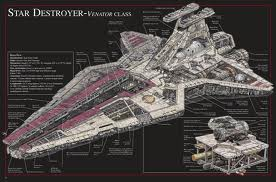
\includegraphics[scale=0.6]{images/starwars.jpeg}}}}{images/starwars.jpeg}
\end{center}
\caption{Un système complexe}
\end{figure}

On parle aussi de \textbf{Système de systèmes} quand un système :
\begin{itemize}

\item{} doit gérer les interactions entre ses parties (ou composantes)



\item{} assure un comportement prévu à l’avance



\item{} gère les comportements (de l’environnement) inatendus


\end{itemize}
\begin{figure}[H]

\begin{center}
\imgexists{images/starwars2.jpeg}{{\imgevalsize{images/starwars2.jpeg}{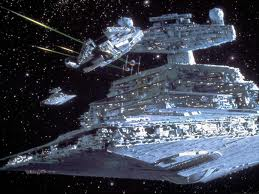
\includegraphics[scale=0.7]{images/starwars2.jpeg}}}}{images/starwars2.jpeg}
\end{center}
\caption{Un système de système}
\end{figure}

\section{Différents types d’analyse}
\label{_différents_types_d_8217_analyse}\hyperlabel{_différents_types_d_8217_analyse}%

Toute la question que l’Ingénierie Système \index{IS} cherche à résoudre est : comment passer des exigences au système
de la façon la plus efficace possible.
\begin{figure}[H]

\begin{center}
\imgexists{images/analyse1.png}{{\imgevalsize{images/analyse1.png}{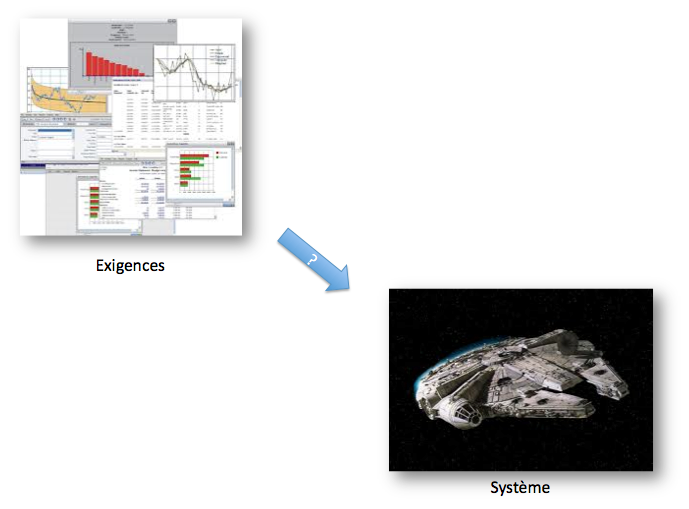
\includegraphics[scale=0.5]{images/analyse1.png}}}}{images/analyse1.png}
\end{center}
\caption{Des exigences au système}
\end{figure}

Pour cela l’Ingénierie Système \index{IS} est découpée en plusieurs analyses, chacune avec un but bien particulier :
\begin{figure}[H]

\begin{center}
\imgexists{images/analyse2.png}{{\imgevalsize{images/analyse2.png}{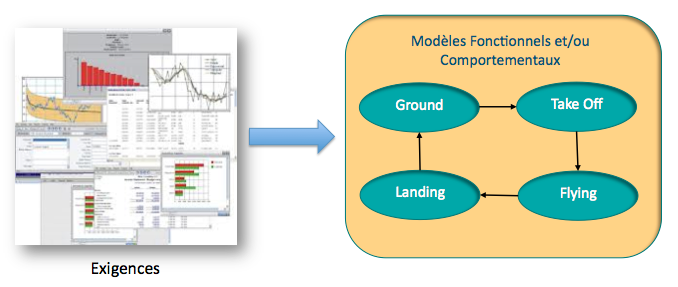
\includegraphics[scale=0.5]{images/analyse2.png}}}}{images/analyse2.png}
\end{center}
\caption{Analyse Fonctionnelle et/ou Comportementale}
\end{figure}
\begin{figure}[H]

\begin{center}
\imgexists{images/analyse3.png}{{\imgevalsize{images/analyse3.png}{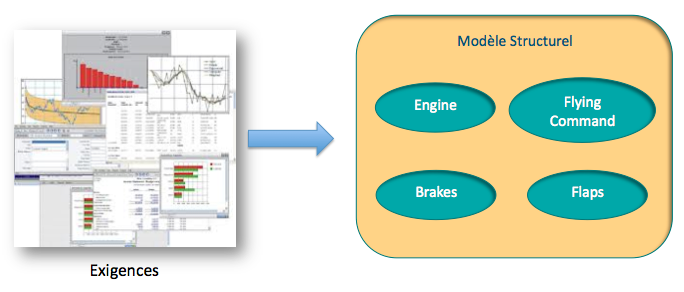
\includegraphics[scale=0.5]{images/analyse3.png}}}}{images/analyse3.png}
\end{center}
\caption{Analyse Structurelle}
\end{figure}
\begin{figure}[H]

\begin{center}
\imgexists{images/analyse4.png}{{\imgevalsize{images/analyse4.png}{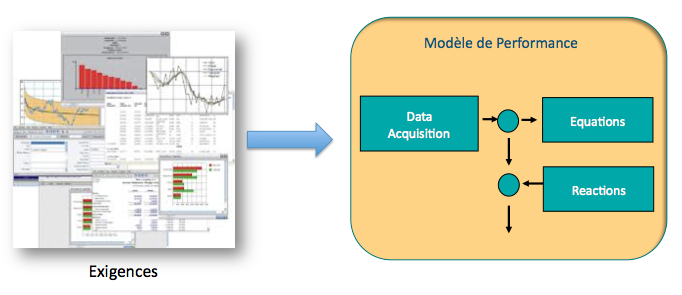
\includegraphics[scale=0.5]{images/analyse4.png}}}}{images/analyse4.png}
\end{center}
\caption{Analyse de performance}
\end{figure}
\begin{figure}[H]

\begin{center}
\imgexists{images/analyse5.png}{{\imgevalsize{images/analyse5.png}{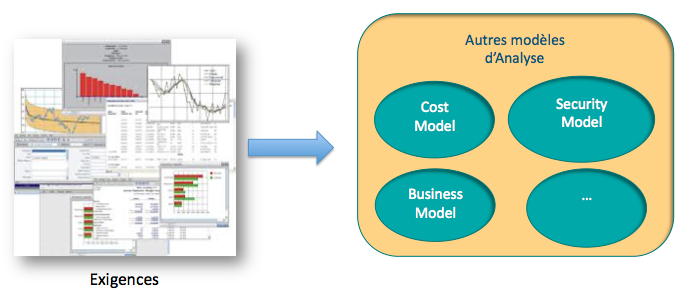
\includegraphics[scale=0.5]{images/analyse5.png}}}}{images/analyse5.png}
\end{center}
\caption{Analyses spécifiques}
\end{figure}

Pour arriver à combler le gap entre le système à développer et ses spécifications.
\begin{figure}[H]

\begin{center}
\imgexists{images/analyse6.png}{{\imgevalsize{images/analyse6.png}{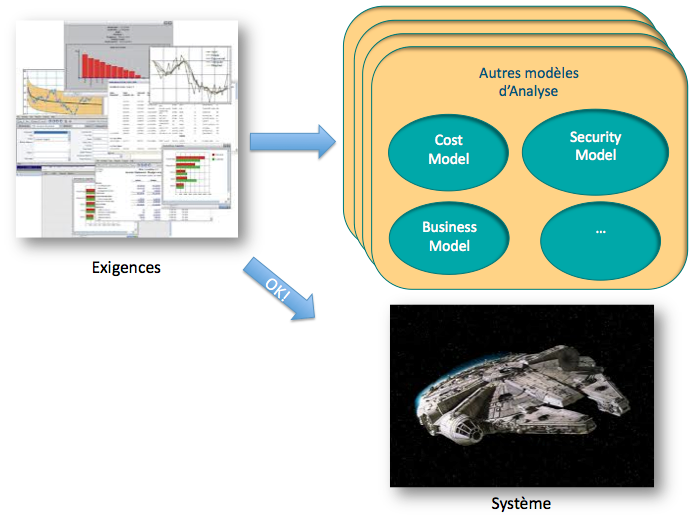
\includegraphics[scale=0.5]{images/analyse6.png}}}}{images/analyse6.png}
\end{center}
\caption{Des exigences au système}
\end{figure}

% ------- 
% Chapter 
% ------- 

\chapter{Normes et standards}
\label{_normes_et_standards}\hyperlabel{_normes_et_standards}%

Il existe un grand nombre de standards en Ingénierie Système \index{IS}. Cette section fera (bientôt) une revue
de ces différents standards et organismes et de leur utilisation (IEEE, EIA, ISO, certification, NASA, INCOSE, AFIS, …).

Enfin, citons un rapport de 2010, le \href{http://www.industrie.gouv.fr/logiciel-embarque/Rapport-BGLE-final.pdf}{Rapport Potier}, qui présente l'état des logiciels embarqués
et qui sera utiles à ceux qui s’intéressent aux verrous technologiques liés à ce domaine.

L’Ingénierie Système \index{IS} génère beaucoup de documentation. Les processus de certification (par exemple dans l’aéronautique) sont
encore basés sur des documents textuels.

% ------- 
% Chapter 
% ------- 

\chapter{Des documents aux modèles}
\label{_des_documents_aux_modèles}\hyperlabel{_des_documents_aux_modèles}%

Vue la complexité grandissante des systèmes, petit à petit cette ingénierie tente de passer d’une
ingénierie \textbf{centrée documents} à une ingénierie \textbf{centrée modèles}. D’où l’importance de se poser la question
des notations et langages pour réaliser et communiquer avec ces modèles (cf. Chapitre \ref{Notation}).

% ------- 
% Chapter 
% ------- 

\chapter{Les exigences}
\label{exigences}\hyperlabel{exigences}%

L’ingénierie des exigences est d’une importance capitale en Ingénierie Système \index{IS}.
Nous renvoyons pour l’instant le lecteur au cours de Master qui précède ce cours.
\begin{figure}[H]

\begin{center}
\imgexists{images/ingenierie-des-exigences.jpg}{{\imgevalsize{images/ingenierie-des-exigences.jpg}{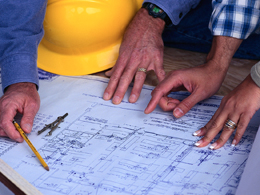
\includegraphics[scale=0.6]{images/ingenierie-des-exigences.jpg}}}}{images/ingenierie-{}des-{}exigences.jpg}
\end{center}
\caption{300 corps de métiers sont parfois présents sur un chantier}
\end{figure}
\begin{figure}[H]

\begin{center}
\imgexists{./images/ProgrammerHumor.jpg}{{\imgevalsize{./images/ProgrammerHumor.jpg}{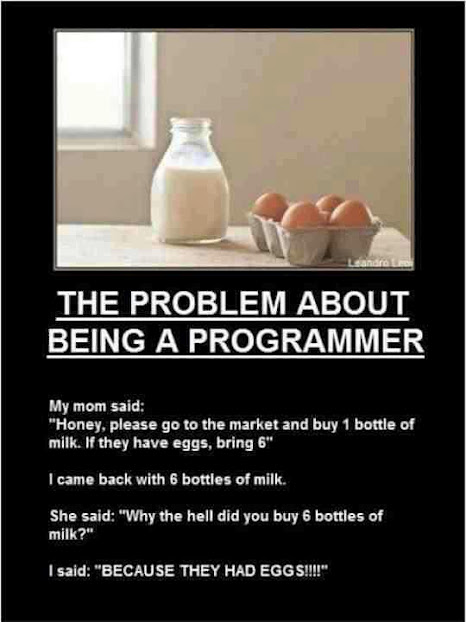
\includegraphics[scale=0.5]{./images/ProgrammerHumor.jpg}}}}{./images/ProgrammerHumor.jpg}
\end{center}
\caption[{Humour (taken from here)}]{Humour (taken from \href{https://plus.google.com/100035762233109552669/posts/a8Hafq2hZ74}{here})}
\label{fig:eggs}\hyperlabel{fig:eggs}%
\end{figure}

% ------- 
% Chapter 
% ------- 

\chapter{L’architecture du système}
\label{structure}\hyperlabel{structure}%

Liens avec AADL, …

% ------- 
% Chapter 
% ------- 

\chapter{Le comportement du système}
\label{comportement}\hyperlabel{comportement}%

Liens avec la V\&V

% ------- 
% Chapter 
% ------- 

\chapter{Méthodes et démarches}
\label{Methodes}\hyperlabel{Methodes}%

\index{Méthodes}

SysML n’est pas une méthode. En effet aucune démarche n’est imposée pour
l’utilisation des diagrammes, l’ordre logique dans lesquels il vaut mieux les réaliser, etc. La spécification ne porte que sur la notation elle-{}même. D’où le pluriel dans le titre de cette section : il existe presque autant de méthodes que d’entreprise développant des systèmes.
Nous nous contenterons de donner ici quelques heuristiques (cf. Annexe \hyperlink{methodo}{Considérations méthodologiques} pour la présentation de quelques méthodes bien identifiées) :

\begin{longfloat}{example}{\caption{Approche itérative}
}

Un diagramme ne doit pas être considéré comme définitif. Il peut être complété alors que l’on traite un autre aspect de la modélisation (exemple classique : ajout d’un nouveau bloc lors de la réalisation d’un diagramme de séquence). Quelque soit la démarche adoptée elle doit être \textbf{itérative} et permettre de revenir sur les premières étapes.

\end{longfloat}

\begin{longfloat}{example}{\caption{Niveau d’abstraction}
}

Bien intégrer les niveaux d’abstraction dans votre démarche. SysML possède certaines constructions pour formaliser cet aspect (\texttt{Pac\penalty5000 k\penalty5000 a\penalty5000 ges} par exemple). Nous matérialisons cet aspect par la partie verticale de la matrice (cf. Tableau \ref{Matrice}).

\end{longfloat}

\begin{longfloat}{example}{\caption{Tous les diagrammes ne sont pas utiles}
}

N’essayez pas de réaliser tous les diagrammes possibles pour votre système. Réalisez uniquement ceux qui sont utiles à votre cas particulier.

\end{longfloat}
%
% PART
%

\part{Partie 3 : La notation SysML}
\label{_partie_3_la_notation_sysml}\hyperlabel{_partie_3_la_notation_sysml}%

% ------- 
% Chapter 
% ------- 

\chapter{Pourquoi une nouvelle notation}
\label{Notation}\hyperlabel{Notation}%
\begin{quote}

A good notation has subtlety and suggestiveness which at times makes
it almost seem like a live teacher.

\hspace*\fill--- Bertrand Russell
\emph{The World of Mathematics (1956)} \end{quote}

Il existe une notation qui se veut "unifiée" pour les modèles : \href{http://www.uml.org/}{UML}\index{UML}.
Néanmoins cette notation est peu adaptée pour l’Ingénierie Système \index{IS} :
\begin{itemize}

\item{} UML 1.x était complètement inadaptée :

\begin{itemize}

\item{} Principalement pour les systèmes d’information



\item{} Peu de liens entre les diagrammes



\item{} Peu de liens entre les modèles et les exigences


\end{itemize}


\item{} UML 2.x n’est pas beaucoup mieux si ce n’est :

\begin{itemize}

\item{} Implication des ingénieurs systèmes pour sa définition



\item{} Introduction du diagramme de structure composite


\end{itemize}

\end{itemize}

En conclusion \href{http://www.uml.org/}{UML}\index{UML} est une bonne base :
\begin{itemize}

\item{} Standard \emph{De facto} en génie logiciel



\item{} Fournit beaucoup de concepts utiles pour décrire des systèmes (même complexes)



\item{} Stable et extensible (grâce notamment au mécanisme de \emph{profile})



\item{} Beaucoup d’outils disponibles


\end{itemize}

Mais…
\begin{itemize}

\item{} Manque de certains concepts clés d’Ingénierie Système \index{IS} 


\item{} Vocabulaire beaucoup trop « software » pour être utilisé par les ingénieurs systèmes (concept de \texttt{cla\penalty5000 sse} ou d'\texttt{hér\penalty5000 i\penalty5000 t\penalty5000 age} par exemple)



\item{} Trop de diagrammes (13 sortes)


\end{itemize}

% ------- 
% Chapter 
% ------- 

\chapter{Introduction à SysML}
\label{_introduction_à_sysml}\hyperlabel{_introduction_à_sysml}%

\section{Fiche d’identité}
\label{_fiche_d_8217_identité_2}\hyperlabel{_fiche_d_8217_identité_2}%


\begin{sidebar}
\begin{itemize}

\item{} Date de naissance non officielle : 2001!



\item{} Première spécification adoptée à l’\href{http://www.omg.org}{OMG}\index{OMG} : 19 septembre 2007



\item{} Version actuelle : \href{http://www.sysml.org/docs/specs/OMGSysML-v1.3-12-06-02.pdf}{1.3} (12/06/2012)



\item{} Paternité : \href{http://www.omg.org}{OMG}\index{OMG}/\href{http://www.uml.org/}{UML}\index{UML} + \href{http://www.incose.org/}{INCOSE}\index{INCOSE} 


\item{} Auteurs principaux :

\begin{itemize}

\item{} Conrad Bock



\item{} Cris Kobryn



\item{} Sanford Friedenthal


\end{itemize}

\end{itemize}
\end{sidebar}

\section{Différence avec UML}
\label{_différence_avec_uml}\hyperlabel{_différence_avec_uml}%
\begin{figure}[H]

\begin{center}
\imgexists{images/diff.png}{{\imgevalsize{images/diff.png}{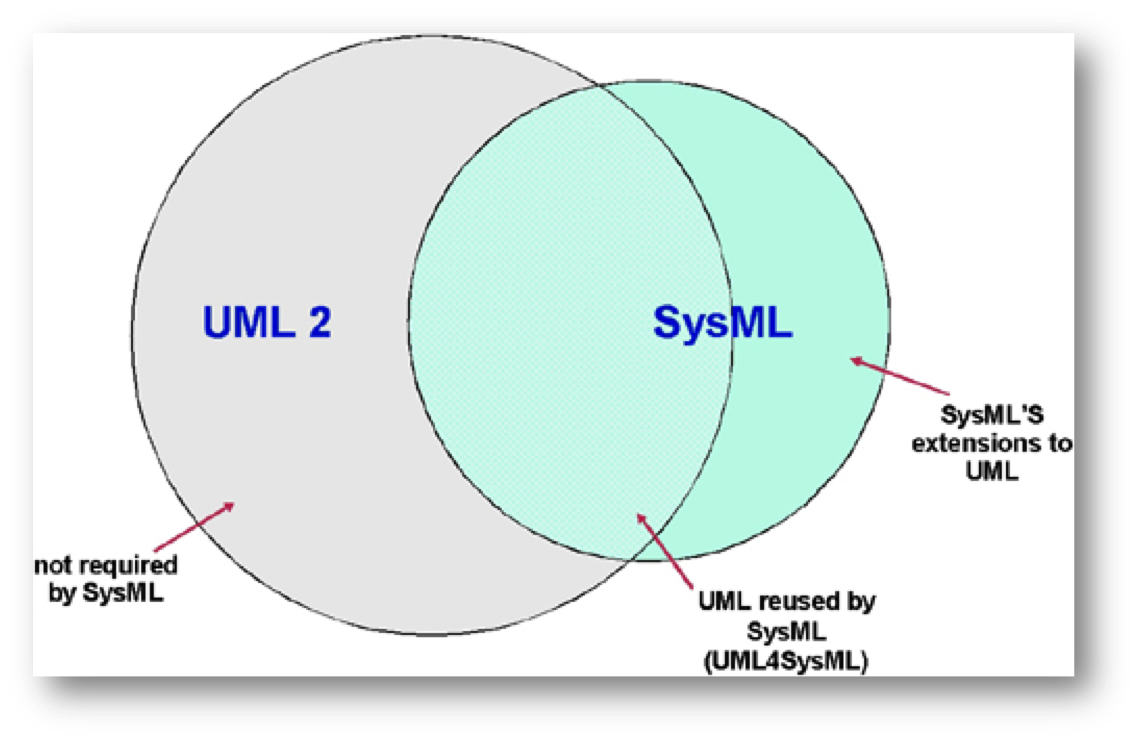
\includegraphics[scale=0.6]{images/diff.png}}}}{images/diff.png}
\end{center}
\caption{Liens entre UML et SysML}
\end{figure}

\section{Qui est "derrière"?}
\label{_qui_est_derrière}\hyperlabel{_qui_est_derrière}%

\noindent
\begin{description}
\item[{ Industrie
}] \hspace{0em}\\
 American Systems, BAE Systems, Boeing, Deere \& Company, EADS Astrium, Eurostep, Israel Aircraft Industries,  Lockheed Martin, Motorola, NIST, Northrop Grumman, oose.de, Raytheon, Thales, …

\item[{ Vendeurs d’outils
}] \hspace{0em}\\
 Artisan, EmbeddedPlus, Gentleware, IBM, Mentor Graphics, PivotPoint Technology, Sparx Systems, Vitech, …

\item[{ Autres organisations
}] \hspace{0em}\\
 AP-{}233, INCOSE, Georgia Institute of Technology, AFIS, …

\end{description}

\section{Organisation des différents diagrammes}
\label{_organisation_des_différents_diagrammes}\hyperlabel{_organisation_des_différents_diagrammes}%
\begin{figure}[H]

\begin{center}
\imgexists{images/Figure4-1.png}{{\imgevalsize{images/Figure4-1.png}{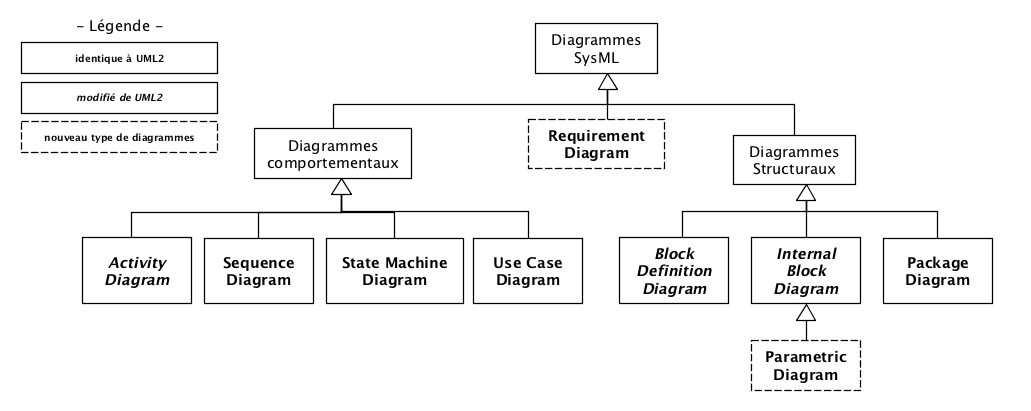
\includegraphics[scale=0.3]{images/Figure4-1.png}}}}{images/Figure4-{}1.png}
\end{center}
\caption{Les 9 diagrammes SysML et leur lien avec UML}
\end{figure}
\begin{figure}[H]

\begin{center}
\imgexists{images/Figure4-1-bis.png}{{\imgevalsize{images/Figure4-1-bis.png}{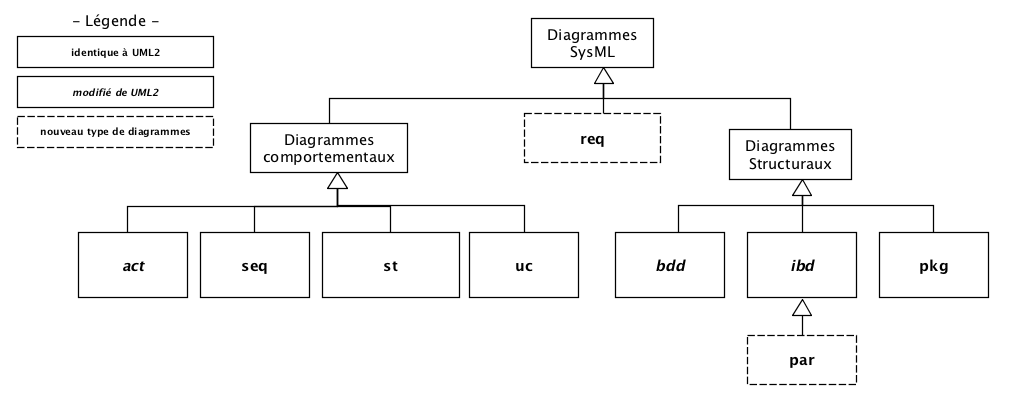
\includegraphics[scale=0.3]{images/Figure4-1-bis.png}}}}{images/Figure4-{}1-{}bis.png}
\end{center}
\caption{Version abrégée des diagrammes}
\end{figure}

\section{Différence entre modèle et dessin}
\label{_différence_entre_modèle_et_dessin}\hyperlabel{_différence_entre_modèle_et_dessin}%

\href{http://www.omgwiki.org/OMGSysML/}{SysML}\index{SysML} n’est pas une palette de dessins et d'éléments de base servant à faire
des diagrammes. Il existe une représentation graphique des éléments modélisés en \href{http://www.omgwiki.org/OMGSysML/}{SysML}\index{SysML}. Elle est importante car elle permet de communiquer visuellement sur le système en développement, mais du point de vue du concepteur, c’est \textbf{le modèle} qui importe le plus.

C’est pourquoi nous vous recommandons de ne jamais "dessiner" des diagrammes \href{http://www.omgwiki.org/OMGSysML/}{SysML}\index{SysML} \footnote{
Sauf bien sûr au brouillon ou sur un tableau, notamment quand on travaille en équipe.
}, mais d’utiliser des outils dédiés (cf. section Chapitre \ref{Outils}).

Pour ceux qui cherchent à étudier un diagramme en particulier voici un plan de cette section (nous utilisons ici le "plan" vu lors de l’introduction de la Tableau \ref{Matrice}) :
\begin{center}
\begingroup%
\setlength{\newtblsparewidth}{\linewidth-2\tabcolsep-2\tabcolsep-2\tabcolsep-2\tabcolsep-2\tabcolsep-2\tabcolsep}%
\setlength{\newtblstarfactor}{\newtblsparewidth / \real{100}}%

\begin{longtable}{lllll}\caption[{Organisation}]{Organisation}\tabularnewline
\hline
\multicolumn{1}{|p{20\newtblstarfactor}|}{\raggedright\bfseries%
%
 %
}&\multicolumn{1}{p{20\newtblstarfactor}|}{\raggedright\bfseries%
%
 Requirements, cf. Chapitre \ref{reqs} %
}&\multicolumn{1}{p{20\newtblstarfactor}|}{\raggedright\bfseries%
%
 Structure, cf. Chapitre \ref{archi} %
}&\multicolumn{1}{p{20\newtblstarfactor}|}{\raggedright\bfseries%
%
 Comportement, cf. Section \ref{behavior} %
}&\multicolumn{1}{p{20\newtblstarfactor}|}{\raggedright\bfseries%
%
 Transverse, cf. Chapitre \ref{transvers}%
}\tabularnewline
\cline{1-1}\cline{2-2}\cline{3-3}\cline{4-4}\cline{5-5}\endfirsthead
\caption[]{(continued)}\tabularnewline
\hline
\multicolumn{1}{|p{20\newtblstarfactor}|}{\raggedright\bfseries%
%
 %
}&\multicolumn{1}{p{20\newtblstarfactor}|}{\raggedright\bfseries%
%
 Requirements, cf. Chapitre \ref{reqs} %
}&\multicolumn{1}{p{20\newtblstarfactor}|}{\raggedright\bfseries%
%
 Structure, cf. Chapitre \ref{archi} %
}&\multicolumn{1}{p{20\newtblstarfactor}|}{\raggedright\bfseries%
%
 Comportement, cf. Section \ref{behavior} %
}&\multicolumn{1}{p{20\newtblstarfactor}|}{\raggedright\bfseries%
%
 Transverse, cf. Chapitre \ref{transvers}%
}\tabularnewline
\cline{1-1}\cline{2-2}\cline{3-3}\cline{4-4}\cline{5-5}\endhead
\multicolumn{1}{|p{20\newtblstarfactor}|}{\raggedright%
\textbf{Organisation}
%
}&\multicolumn{1}{p{20\newtblstarfactor}|}{\raggedright%
\texttt{pkg}
%
}&\multicolumn{1}{p{20\newtblstarfactor}|}{\raggedright%
\texttt{pkg}, \texttt{bdd}
%
}&\multicolumn{1}{p{20\newtblstarfactor}|}{\raggedright%
\texttt{pkg}
%
}&\multicolumn{1}{p{20\newtblstarfactor}|}{\raggedright%
%
}\tabularnewline
\cline{1-1}\cline{2-2}\cline{3-3}\cline{4-4}\cline{5-5}\multicolumn{1}{|p{20\newtblstarfactor}|}{\raggedright%
\textbf{Analyse, Conception, Implémentation \footnotemark{}}
%
}&\multicolumn{1}{p{20\newtblstarfactor}|}{\raggedright%
\texttt{req}
%
}&\multicolumn{1}{p{20\newtblstarfactor}|}{\raggedright%
\texttt{bdd}, \texttt{ibd}, \texttt{seq}, \texttt{par}
%
}&\multicolumn{1}{p{20\newtblstarfactor}|}{\raggedright%
\texttt{uc}, \texttt{seq}, \texttt{st}, \texttt{act}
%
}&\multicolumn{1}{p{20\newtblstarfactor}|}{\raggedright%
\texttt{par}
%
}\tabularnewline
\hline
\end{longtable}\endgroup%

\end{center}
\addtocounter{footnote}{-1}\stepcounter{footnote}
\footnotetext{
En fonction du niveau de détail.
}
% ------- 
% Chapter 
% ------- 

\chapter{Outils SysML}
\label{Outils}\hyperlabel{Outils}%

Il existe un certain nombre d’outils permettant de réaliser des modèles SysML. Voici une liste non exhaustive :
\begin{itemize}

\item{} \href{http://www.topcased.org/}{TopCased} 


\item{} \href{http://www.eclipse.org/modeling/mdt/papyrus/}{Papyrus} 


\item{} \href{http://www.artisansw.com/}{Artisan} 


\item{} \href{http://www-01.ibm.com/software/rational/products/rhapsody}{Rhapsody} 


\item{} \href{http://www.modeliosoft.com/}{Modelio} 


\item{} …


\end{itemize}

Vous trouverez sur Internet des comparatifs et des avis à jour sur les outils.

Ce que je voudrai souligner ici c’est l’importance du modèle comme "dépôt" (je préfère le terme anglais de \emph{repository}) d'éléments de base en relation les uns avec les autres. C’est toute la différence entre le dessin et le modèle.
\begin{DBKadmonition}{images/icons/important.png}{Important}

Attention toutefois à ne pas confondre ce que vous permet (ou pas) de faire l’outil et la notation elle-{}même. Les fabricants ont parfois pris des libertés ou bien n’ont pas complètement implémenté toutes les subtilités de la notation.
\end{DBKadmonition}

% ------- 
% Chapter 
% ------- 

\chapter{Principes de base}
\label{_principes_de_base}\hyperlabel{_principes_de_base}%

Abordons quelques principes généraux de \href{http://www.omgwiki.org/OMGSysML/}{SysML}\index{SysML}.
\begin{itemize}

\item{} Chaque diagramme \href{http://www.omgwiki.org/OMGSysML/}{SysML}\index{SysML} représente un élément de modélisation



\item{} Chaque diagramme \href{http://www.omgwiki.org/OMGSysML/}{SysML}\index{SysML} doit être incluse dans un cadre (\emph{Diagram Frame})



\item{} L’entête du cadre, appelé \textbf{cartouche}, indique les informations sur le diagramme:

\begin{itemize}

\item{} le type de diagramme (\texttt{req}, \texttt{act}, \texttt{bdd}, \texttt{ibd}, \texttt{sd}, etc.)



\item{} le type d'élément (\emph{package}, \emph{block}, \emph{activity}, etc.)



\item{} le nom de l'élément



\item{} le nom du diagramme ou de la vue


\end{itemize}

\end{itemize}

Dans l’exemple ci-{}dessous, le diagramme "\emph{Context\_Overview}" est un \emph{Block Definition Diagram} (type \texttt{bdd}) qui représente un
\emph{package}, nommé "Context".
\begin{figure}[H]

\begin{center}
\imgexists{images/pacemaker-context.png}{{\imgevalsize{images/pacemaker-context.png}{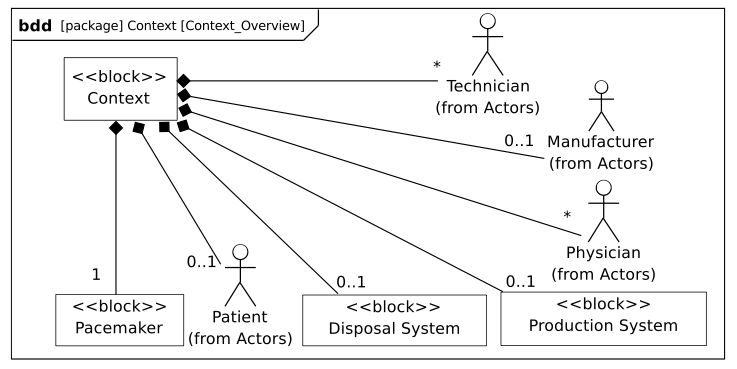
\includegraphics[scale=0.5]{images/pacemaker-context.png}}}}{images/pacemaker-{}context.png}
\end{center}
\caption{Exemple de diagramme SysML}
\end{figure}

% ------- 
% Chapter 
% ------- 

\chapter{Organisation}
\label{org}\hyperlabel{org}%

\section{Fondements}
\label{_fondements}\hyperlabel{_fondements}%

On abordera :
\begin{itemize}

\item{} Le \emph{Package Diagram} 


\item{} Les différent types de \emph{packages} 


\item{} Les organisations possibles



\item{} La notion de \emph{Namespaces} 


\item{} Les \emph{Dependencies} 

\end{itemize}

\section{Le \emph{Package Diagram}}
\label{package}\hyperlabel{package}%
\begin{itemize}

\item{} Identique à \href{http://www.uml.org/}{UML}\index{UML}, et classique pour les développeurs (java notamment)



\item{} Permet d’organiser les modèles en créant un espace de nommage (cf Section \ref{namespace})


\end{itemize}

Les modèles peuvent être organisés selon toutes sortes de considération (cf. Section \ref{organisation}).
Le mécanisme qui permet de les organiser est le \emph{package} (paquetage).
\begin{itemize}

\item{} hiérarchie "système" (e.g., entreprise, système, composant)



\item{} types de diagrammes (e.g., besoins, structure, comportements)



\item{} par points de vue



\item{} etc.


\end{itemize}

\section{Les différent types de \emph{packages}}
\label{_les_différent_types_de_emphasis_packages_emphasis}\hyperlabel{_les_différent_types_de_emphasis_packages_emphasis}%

Il existe plusieurs types de \emph{package} :

\noindent
\begin{description}
\item[{ models
}] \hspace{0em}\\
         un \emph{package} "top-{}level" dans une hiérarchie de \emph{package} 
\item[{ packages
}] \hspace{0em}\\
         le type le plus classique : un ensemble d'éléments de modèles

\item[{ model librairies
}] \hspace{0em}\\
         un \emph{package} prévu pour être réutilisé (importé) par d’autres éléments

\item[{ views
}] \hspace{0em}\\
         un \emph{package} spécial pour représenter les points de vue

\end{description}
\begin{DBKadmonition}{images/icons/note.png}{Note}

Un point de vue (\emph{viewpoint}) est utilisé pour matérialiser une perspective particulière de modélisation.
Il possède des propriétés standardisés (\emph{concerns}, \emph{language}, \emph{purpose}, etc.) et permettent d’indiquer qu’une
vue (un \emph{packetage} particulier, stéréotypé \texttt{<{}<{}v\penalty5000 i\penalty5000 e\penalty5000 w>{}>{}}) est conforme (dépendance \texttt{<{}<{}c\penalty5000 o\penalty5000 n\penalty5000 f\penalty5000 o\penalty5000 r\penalty5000 m>{}>{}}) à un point de vue.
\end{DBKadmonition}

\section{Les organisations possibles}
\label{organisation}\hyperlabel{organisation}%

Les modèles peuvent être organisés selon toutes sortes de considération :
\begin{itemize}

\item{} par hiérarchie "système" (e.g., entreprise, système, composant, …)



\item{} par types de diagrammes (e.g., besoins, structure, comportements, …)



\item{} par cycle de vie (e.g., analyse, conception, …)



\item{} par équipes (e.g., architectes, \hyperlink{IPT}{[IPT]}, …)



\item{} par points de vue (e.g., sécurité, performance, …)



\item{} etc.


\end{itemize}
\begin{figure}[H]

\begin{center}
\imgexists{images/pkg-organisation2.png}{{\imgevalsize{images/pkg-organisation2.png}{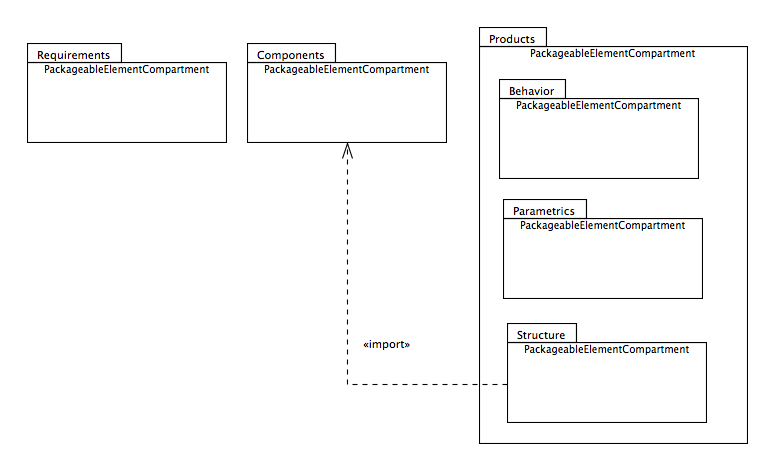
\includegraphics[scale=0.6]{images/pkg-organisation2.png}}}}{images/pkg-{}organisation2.png}
\end{center}
\caption{Exemple d’organisation}
\end{figure}
\begin{figure}[H]

\begin{center}
\imgexists{images/pkg-organisation-modelview.png}{{\imgevalsize{images/pkg-organisation-modelview.png}{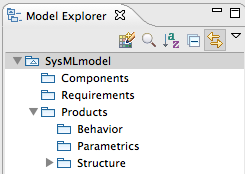
\includegraphics[scale=0.4]{images/pkg-organisation-modelview.png}}}}{images/pkg-{}organisation-{}modelview.png}
\end{center}
\caption{Exemple d’organisation}
\end{figure}
\begin{figure}[H]

\begin{center}
\imgexists{images/pkg-organisation.png}{{\imgevalsize{images/pkg-organisation.png}{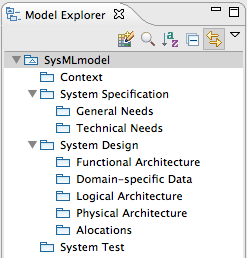
\includegraphics[scale=0.4]{images/pkg-organisation.png}}}}{images/pkg-{}organisation.png}
\end{center}
\caption{Exemple d’organisation}
\end{figure}
\begin{figure}[H]

\begin{center}
\imgexists{images/pkg-topcased.png}{{\imgevalsize{images/pkg-topcased.png}{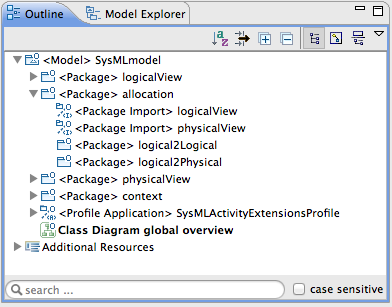
\includegraphics[scale=0.4]{images/pkg-topcased.png}}}}{images/pkg-{}topcased.png}
\end{center}
\caption{Exemple d’organisation}
\end{figure}
\begin{DBKadmonition}{images/icons/note.png}{Organisation par défaut}

L’outil \href{http://www.topcased.org}{TOPCASED}\index{Topcased} propose, lors de la création d’un premier modèle, de créer une organisation
"type" par défaut.

\noindent\imgexists{images/pkg-template.png}{{\imgevalsize{images/pkg-template.png}{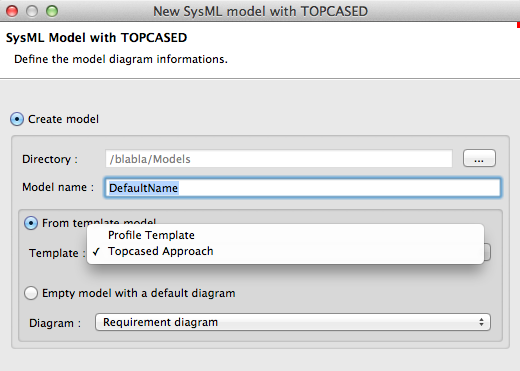
\includegraphics[scale=0.3]{images/pkg-template.png}}}}{images/pkg-{}template.png} \noindent\imgexists{images/pkg-topcased-default.png}{{\imgevalsize{images/pkg-topcased-default.png}{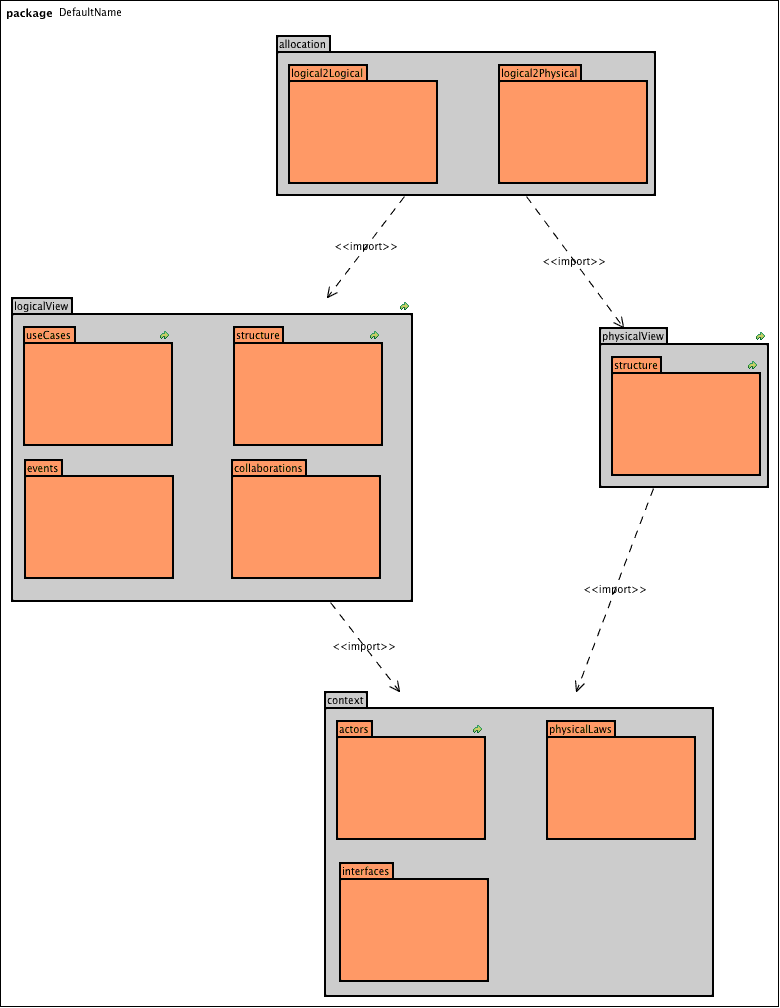
\includegraphics[scale=0.2]{images/pkg-topcased-default.png}}}}{images/pkg-{}topcased-{}default.png}
\end{DBKadmonition}

\section{La notion de \emph{Namespaces}}
\label{namespace}\hyperlabel{namespace}%

Un \emph{package} est un espace de nommage pour tous les éléments qu’il contient.
Ainsi, dans un \emph{package}, on n’a pas à se soucier des noms des éléments. Même si d’autres utilisent les mêmes noms,
il n’y aura pas ambiguité.
\begin{DBKadmonition}{images/icons/note.png}{Définition : Namespace (OMG SysML v1.3, p. 23)}

\emph{The package defines a namespace for the packageable elements.}
\end{DBKadmonition}
\begin{DBKadmonition}{images/icons/note.png}{Note}

Dans les outils \href{http://www.omgwiki.org/OMGSysML/}{SysML}\index{SysML}, vous pouvez demander à voir les noms complets (\emph{Qualified names})
des éléments, c’est à dire le nom de l'élément prefixé par son (ou ses) \emph{package(s)} (e.g., \texttt{Str\penalty5000 u\penalty5000 c\penalty5000 t\penalty5000 ure:\penalty0 :\penalty0 Pro\penalty5000 d\penalty5000 u\penalty5000 cts:\penalty0 :\penalty0 Clock}).
\end{DBKadmonition}

\section{Les dépendances}
\label{_les_dépendances}\hyperlabel{_les_dépendances}%

Un certain nombre de dépendances peuvent exister entre des éléments de \emph{package} ou entre les \emph{packages} eux-{}mêmes :

\noindent
\begin{description}
\item[{ \emph{Dependency} }] \hspace{0em}\\
         une dépendance "générale", non précisée,\newline
         représentée par une simple flèche pointillée \texttt{-{}\penalty0 -{}\penalty0 -{}\penalty0 -{}\penalty0 -{}\penalty0 >{}} 
\item[{ \emph{Use} }] \hspace{0em}\\
         l'élément "utilise" celui à l’autre bout de la flèche (un type par exemple),\newline
         représentée par le stéréotype \texttt{<{}<{}u\penalty5000 s\penalty5000 e>{}>{}} 
\item[{ \emph{Refine} }] \hspace{0em}\\
         l'élément est un raffinage (plus détaillé) de celui à l’autre bout de la flèche,\newline
         représentée par le stéréotype \texttt{<{}<{}r\penalty5000 e\penalty5000 f\penalty5000 i\penalty5000 n\penalty5000 e>{}>{}} 
\item[{ \emph{Realization} }] \hspace{0em}\\
         l'élément est une "réalisation" (implémentation) de celui à l’autre bout de la flèche,\newline
         représentée par le stéréotype \texttt{<{}<{}r\penalty5000 e\penalty5000 a\penalty5000 l\penalty5000 i\penalty5000 z\penalty5000 e>{}>{}} 
\item[{ \emph{Allocation} }] \hspace{0em}\\
         l'élément (e.g., une activité ou un \emph{requirement}) est "alloué" sur celui à l’autre bout de la flèche (un \texttt{block} la plupart du temps),\newline
         représentée par le stéréotype \texttt{<{}<{}a\penalty5000 l\penalty5000 l\penalty5000 o\penalty5000 c\penalty5000 a\penalty5000 t\penalty5000 e>{}>{}} 
\end{description}

\section{En résumé}
\label{_en_résumé}\hyperlabel{_en_résumé}%

\href{http://www.omgwiki.org/OMGSysML/}{SysML}\index{SysML} propose un certain nombre de mécanismes pour organiser les différents modèles,
tirés pour la plupart d’\href{http://www.uml.org/}{UML}\index{UML}. Ces mécanismes seront plus faciles à comprendre au travers
de leur utilisation concrète dans la suite.
\begin{center}
\begingroup%
\setlength{\newtblsparewidth}{\linewidth-2\tabcolsep-2\tabcolsep-2\tabcolsep-2\tabcolsep-2\tabcolsep-2\tabcolsep}%
\setlength{\newtblstarfactor}{\newtblsparewidth / \real{100}}%

\begin{longtable}{lllll}\caption[{Organisation}]{Organisation}\tabularnewline
\hline
\multicolumn{1}{|p{20\newtblstarfactor}|}{\raggedright\bfseries%
%
 %
}&\multicolumn{1}{p{20\newtblstarfactor}|}{\raggedright\bfseries%
%
 Requirements        %
}&\multicolumn{1}{p{20\newtblstarfactor}|}{\raggedright\bfseries%
%
 Structure   %
}&\multicolumn{1}{p{20\newtblstarfactor}|}{\raggedright\bfseries%
%
 Comportement    %
}&\multicolumn{1}{p{20\newtblstarfactor}|}{\raggedright\bfseries%
%
 Transverse%
}\tabularnewline
\cline{1-1}\cline{2-2}\cline{3-3}\cline{4-4}\cline{5-5}\endfirsthead
\caption[]{(continued)}\tabularnewline
\hline
\multicolumn{1}{|p{20\newtblstarfactor}|}{\raggedright\bfseries%
%
 %
}&\multicolumn{1}{p{20\newtblstarfactor}|}{\raggedright\bfseries%
%
 Requirements        %
}&\multicolumn{1}{p{20\newtblstarfactor}|}{\raggedright\bfseries%
%
 Structure   %
}&\multicolumn{1}{p{20\newtblstarfactor}|}{\raggedright\bfseries%
%
 Comportement    %
}&\multicolumn{1}{p{20\newtblstarfactor}|}{\raggedright\bfseries%
%
 Transverse%
}\tabularnewline
\cline{1-1}\cline{2-2}\cline{3-3}\cline{4-4}\cline{5-5}\endhead
\multicolumn{1}{|p{20\newtblstarfactor}|}{\raggedright%
\textbf{\textbf{Organisation}}
%
}&\multicolumn{1}{p{20\newtblstarfactor}|}{\raggedright%
\texttt{pac\penalty5000 k\penalty5000 age}
%
}&\multicolumn{1}{p{20\newtblstarfactor}|}{\raggedright%
\texttt{pac\penalty5000 k\penalty5000 age}
%
}&\multicolumn{1}{p{20\newtblstarfactor}|}{\raggedright%
\texttt{pac\penalty5000 k\penalty5000 age}
%
}&\multicolumn{1}{p{20\newtblstarfactor}|}{\raggedright%
\texttt{dep\penalty5000 e\penalty5000 n\penalty5000 d\penalty5000 e\penalty5000 n\penalty5000 c\penalty5000 ies}
%
}\tabularnewline
\cline{1-1}\cline{2-2}\cline{3-3}\cline{4-4}\cline{5-5}\multicolumn{1}{|p{20\newtblstarfactor}|}{\raggedright%
\textbf{Analyse}
%
}&\multicolumn{1}{p{20\newtblstarfactor}|}{\raggedright%
%
}&\multicolumn{1}{p{20\newtblstarfactor}|}{\raggedright%
%
}&\multicolumn{1}{p{20\newtblstarfactor}|}{\raggedright%
%
}&\multicolumn{1}{p{20\newtblstarfactor}|}{\raggedright%
%
}\tabularnewline
\cline{1-1}\cline{2-2}\cline{3-3}\cline{4-4}\cline{5-5}\multicolumn{1}{|p{20\newtblstarfactor}|}{\raggedright%
\textbf{Conception}
%
}&\multicolumn{1}{p{20\newtblstarfactor}|}{\raggedright%
%
}&\multicolumn{1}{p{20\newtblstarfactor}|}{\raggedright%
%
}&\multicolumn{1}{p{20\newtblstarfactor}|}{\raggedright%
%
}&\multicolumn{1}{p{20\newtblstarfactor}|}{\raggedright%
%
}\tabularnewline
\cline{1-1}\cline{2-2}\cline{3-3}\cline{4-4}\cline{5-5}\multicolumn{1}{|p{20\newtblstarfactor}|}{\raggedright%
\textbf{Implémentation}
%
}&\multicolumn{1}{p{20\newtblstarfactor}|}{\raggedright%
%
}&\multicolumn{1}{p{20\newtblstarfactor}|}{\raggedright%
%
}&\multicolumn{1}{p{20\newtblstarfactor}|}{\raggedright%
%
}&\multicolumn{1}{p{20\newtblstarfactor}|}{\raggedright%
%
}\tabularnewline
\hline
\end{longtable}\endgroup%

\end{center}

\section{Questions de révision}
\label{_questions_de_révision}\hyperlabel{_questions_de_révision}%
\begin{enumerate}[label=\arabic*.]

\item{} Quels sont les 5 types de dépendances entre \emph{packageable elements} ?



\item{} À quoi cela peut-{}il servir de définir les dépendances (donnez des exemples concrets) ?


\end{enumerate}

% ------- 
% Chapter 
% ------- 

\chapter{Les exigences}
\label{reqs}\hyperlabel{reqs}%

\section{Fondements}
\label{_fondements_2}\hyperlabel{_fondements_2}%

On abordera :
\begin{itemize}

\item{} L’organization des \emph{Requirements} 


\item{} Les \emph{Requirements properties} 


\item{} Les \emph{Requirements links} 


\item{} Les \emph{Requirements Diagrams} 


\item{} Les considérations sur la traçabilité



\item{} Annotations des \emph{Requirements} 


\item{} Les \emph{Use Case Diagrams} (scénarios)


\end{itemize}
\begin{DBKadmonition}{images/icons/note.png}{Note}

L’ingénierie des exigences est une discipline à part entière et nous n’abordons ici
que les aspects en lien avec la modélisation système. Voir le livre de référence pour
plus de détails (\hyperlink{Sommerville1997}{[Sommerville1997]}) ou le guide de l’AFISindexterm:[AFIS] (\hyperlink{REQ2012}{[REQ2012]}).
\end{DBKadmonition}

\section{L’organisation des \emph{Requirements}}
\label{_l_8217_organisation_des_emphasis_requirements_emphasis}\hyperlabel{_l_8217_organisation_des_emphasis_requirements_emphasis}%

\subsection{Différents types d’organisation}
\label{_différents_types_d_8217_organisation}\hyperlabel{_différents_types_d_8217_organisation}%

Comme nous l’avons vu pour les \emph{packages}, plusieurs types d’organisations sont possibles :
\begin{itemize}

\item{} Par niveau d’abstraction

\begin{itemize}

\item{} Besoins généraux (en lien avec les  \emph{use cases} par exemple)



\item{} Besoins techniques (en lien avec les éléments de conception)


\end{itemize}


\item{} Par point de vue

\begin{itemize}

\item{} Besoins principaux (en lien avec les \emph{use cases})



\item{} Besoins spécifiques :

\begin{itemize}

\item{} Fonctionnels



\item{} Marketing



\item{} Environnementaux



\item{} \emph{Business} 


\item{} …


\end{itemize}

\end{itemize}


\item{} etc.


\end{itemize}

\subsection{Tableaux de \emph{Requirements}}
\label{_tableaux_de_emphasis_requirements_emphasis}\hyperlabel{_tableaux_de_emphasis_requirements_emphasis}%

Les \emph{requirements} sont généralement stockés dans des feuilles excel.
\begin{figure}[H]

\begin{center}
\imgexists{images/req-table.png}{{\imgevalsize{images/req-table.png}{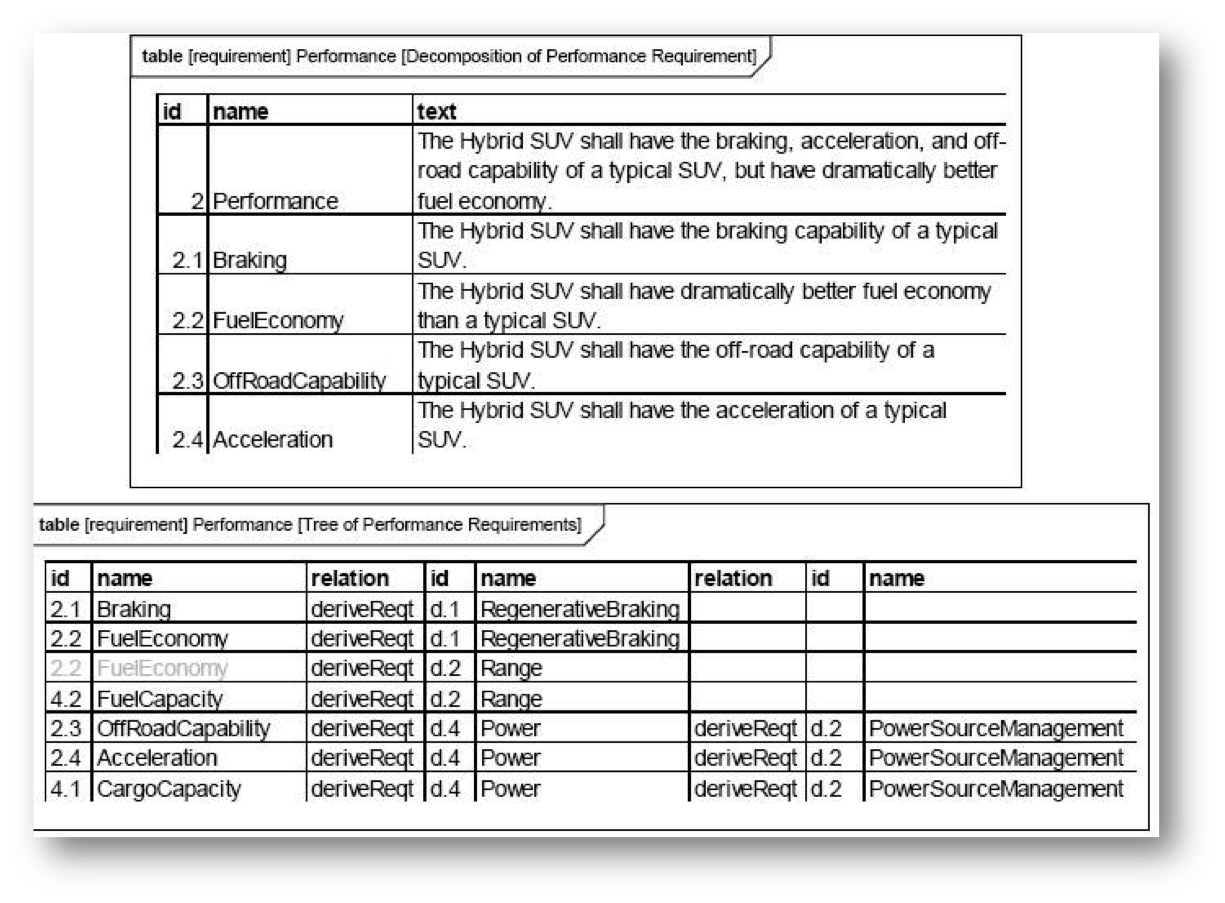
\includegraphics[scale=0.5]{images/req-table.png}}}}{images/req-{}table.png}
\end{center}
\caption{Exemples tableau d’exigences}
\end{figure}
\begin{figure}[H]

\begin{center}
\imgexists{images/req-modelio.png}{{\imgevalsize{images/req-modelio.png}{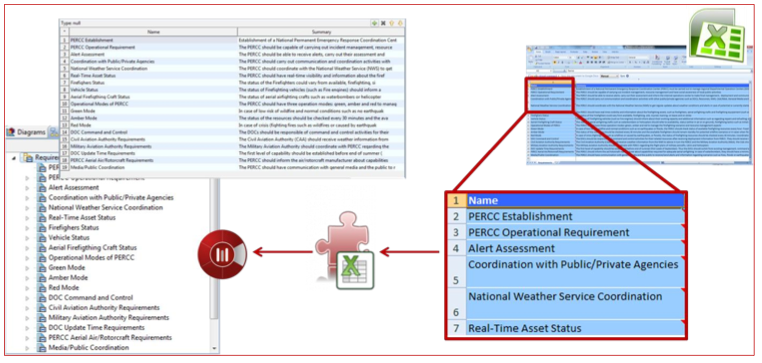
\includegraphics[scale=0.5]{images/req-modelio.png}}}}{images/req-{}modelio.png}
\end{center}
\caption{Import Modelio de tableau d’exigences}
\end{figure}

\section{Les \emph{Requirements properties}}
\label{_les_emphasis_requirements_properties_emphasis}\hyperlabel{_les_emphasis_requirements_properties_emphasis}%

Il est possible d’indiquer un certain nombre de propriétés sur un \emph{requirement} :
\begin{itemize}

\item{} \emph{priority} (\texttt{high}, \texttt{low}, …)



\item{} \emph{source} (\texttt{sta\penalty5000 k\penalty5000 e\penalty5000 o\penalty5000 l\penalty5000 der}, \texttt{law}, \texttt{tec\penalty5000 h\penalty5000 n\penalty5000 i\penalty5000 cal}, …)



\item{} \emph{risk} (\texttt{high}, \texttt{low}, …)



\item{} \emph{status} (\texttt{pro\penalty5000 p\penalty5000 o\penalty5000 sed}, \texttt{apr\penalty5000 o\penalty5000 ved}, …)



\item{} \emph{verification method} (\texttt{ana\penalty5000 l\penalty5000 y\penalty5000 sis}, \texttt{tests}, …)


\end{itemize}

\section{Les \emph{Requirements links}}
\label{_les_emphasis_requirements_links_emphasis}\hyperlabel{_les_emphasis_requirements_links_emphasis}%

Les principales relations entre \emph{requirement} sont :

\noindent
\begin{description}
\item[{ \emph{Containment} }] \hspace{0em}\\
         pour décrire la décomposition d’une exigence en plusieurs sous-{}exigences (⊕–)

\item[{ \emph{Refinement} }] \hspace{0em}\\
         pour décrire un ajout de précision (\texttt{<{}<{}r\penalty5000 e\penalty5000 f\penalty5000 i\penalty5000 n\penalty5000 e>{}>{}})

\item[{ \emph{Derivation} }] \hspace{0em}\\
         pour indiquer une différence de niveau d’abstraction (\texttt{<{}<{}d\penalty5000 e\penalty5000 r\penalty5000 i\penalty5000 v\penalty5000 e\penalty5000 R\penalty5000 e\penalty5000 q\penalty5000 t>{}>{}}), par exemple
        entre un système et un de ses sous-{}systèmes

\end{description}
\begin{DBKadmonition}{images/icons/note.png}{Note}

Lorsqu’un cas d’utilisation possède plusieurs cas \texttt{<{}<{}r\penalty5000 e\penalty5000 f\penalty5000 i\penalty5000 n\penalty5000 e>{}>{}} qui pointent vers lui, on considère que ces différents cas sont des options possibles de raffinement (cf. Chapitre \ref{conventions}).
\end{DBKadmonition}
\begin{figure}[H]

\begin{center}
\imgexists{images/req-exp1.png}{{\imgevalsize{images/req-exp1.png}{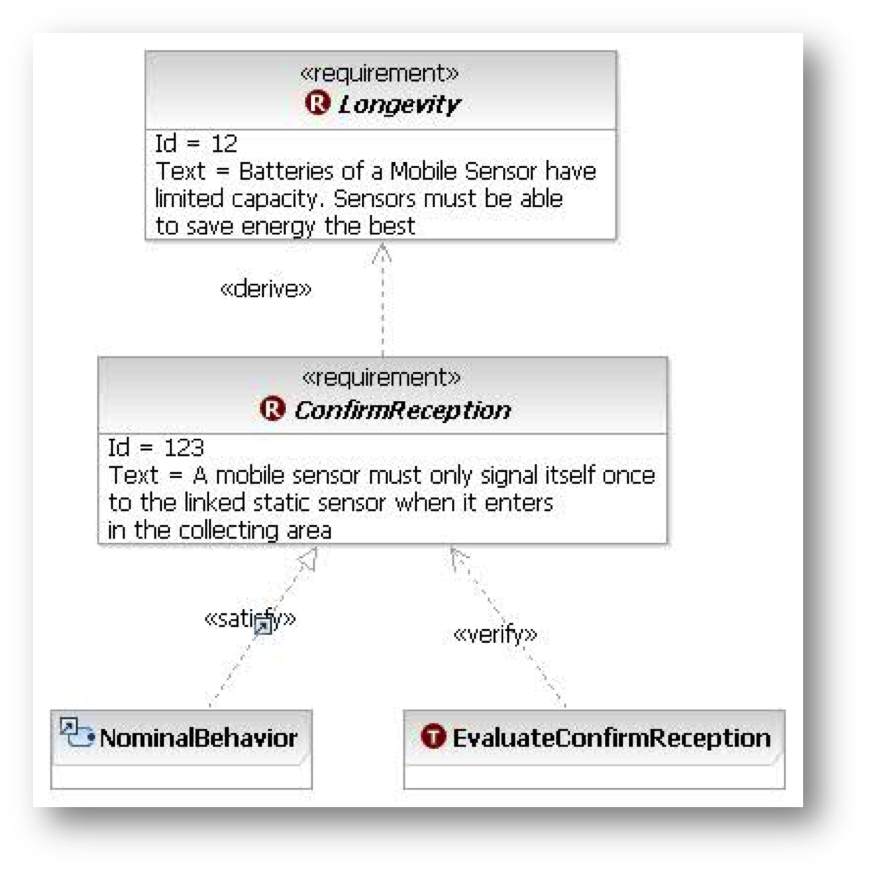
\includegraphics[scale=0.4]{images/req-exp1.png}}}}{images/req-{}exp1.png}
\end{center}
\caption{Exemples de relations entre exigences}
\end{figure}

Il existe ensuite les relations entre les besoins et les autres éléments de modélisation
(les \emph{block} principalement) comme \texttt{<{}<{}s\penalty5000 a\penalty5000 t\penalty5000 i\penalty5000 s\penalty5000 f\penalty5000 y>{}>{}} ou \texttt{<{}<{}v\penalty5000 e\penalty5000 r\penalty5000 i\penalty5000 f\penalty5000 y>{}>{}}, mais nous les aborderons
dans la partie \hyperlink{transvers}{transverse}.
\begin{figure}[H]

\begin{center}
\imgexists{images/topcased-req-connections.png}{{\imgevalsize{images/topcased-req-connections.png}{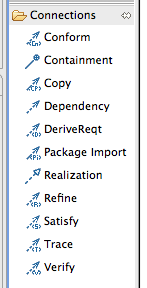
\includegraphics[scale=0.2]{images/topcased-req-connections.png}}}}{images/topcased-{}req-{}connections.png}
\end{center}
\caption{Relations liées au \emph{requirements} dans TOPCASED}
\end{figure}

\section{Les \emph{Requirements Diagrams}}
\label{_les_emphasis_requirements_diagrams_emphasis}\hyperlabel{_les_emphasis_requirements_diagrams_emphasis}%

Quelques exemples de \texttt{req} tirés de \href{http://www.uml-sysml.org/sysml}{http://www.uml-{}sysml.org/\-sysml} :
\begin{figure}[H]

\begin{center}
\imgexists{images/hsuv-reqs1.png}{{\imgevalsize{images/hsuv-reqs1.png}{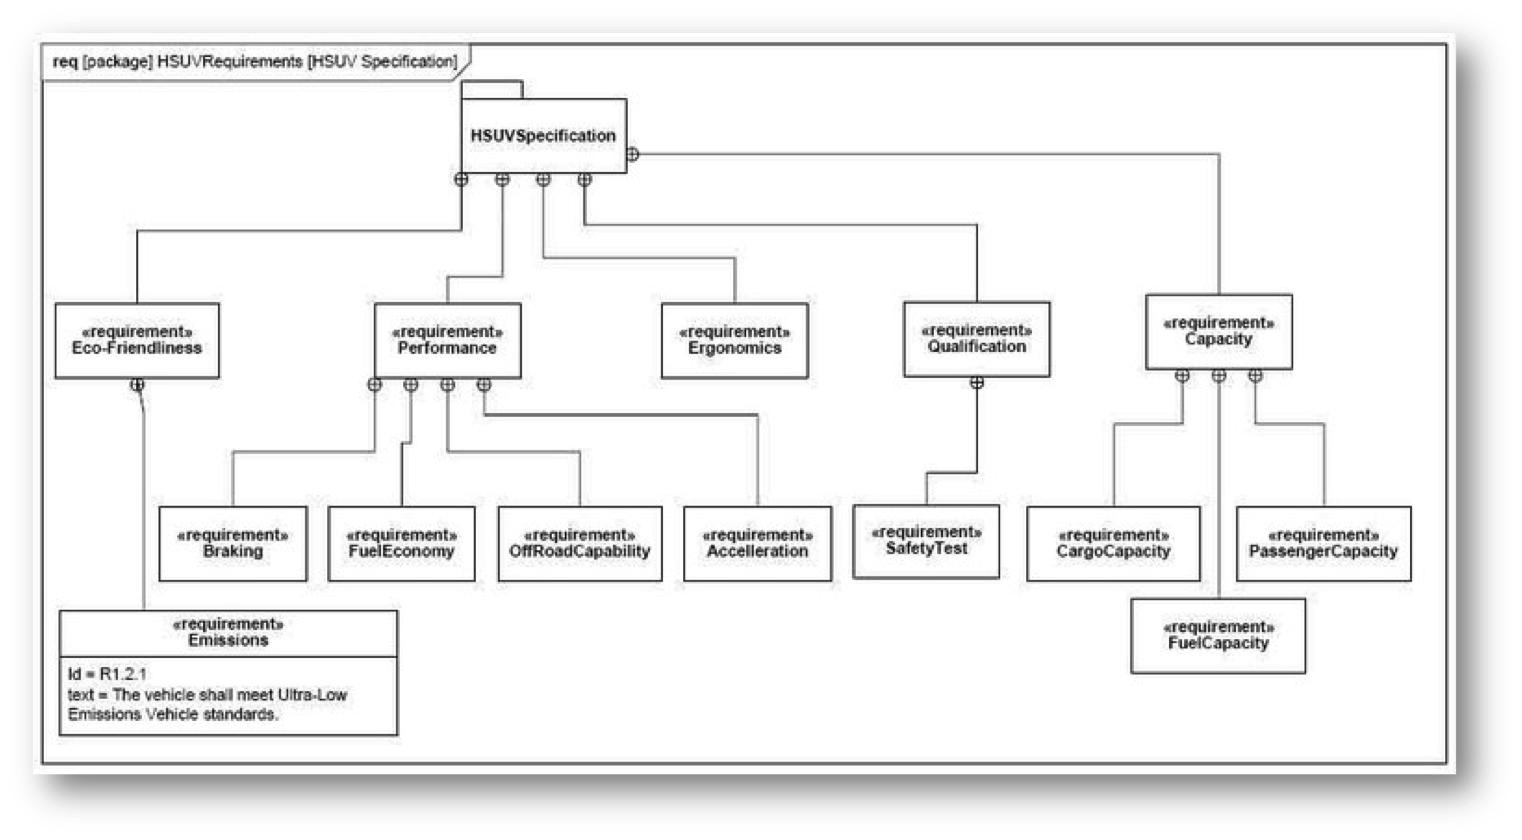
\includegraphics[scale=0.4]{images/hsuv-reqs1.png}}}}{images/hsuv-{}reqs1.png}
\end{center}
\caption{Exemples de composition d’exigences}
\end{figure}
\begin{figure}[H]

\begin{center}
\imgexists{images/hsuv-reqs2.png}{{\imgevalsize{images/hsuv-reqs2.png}{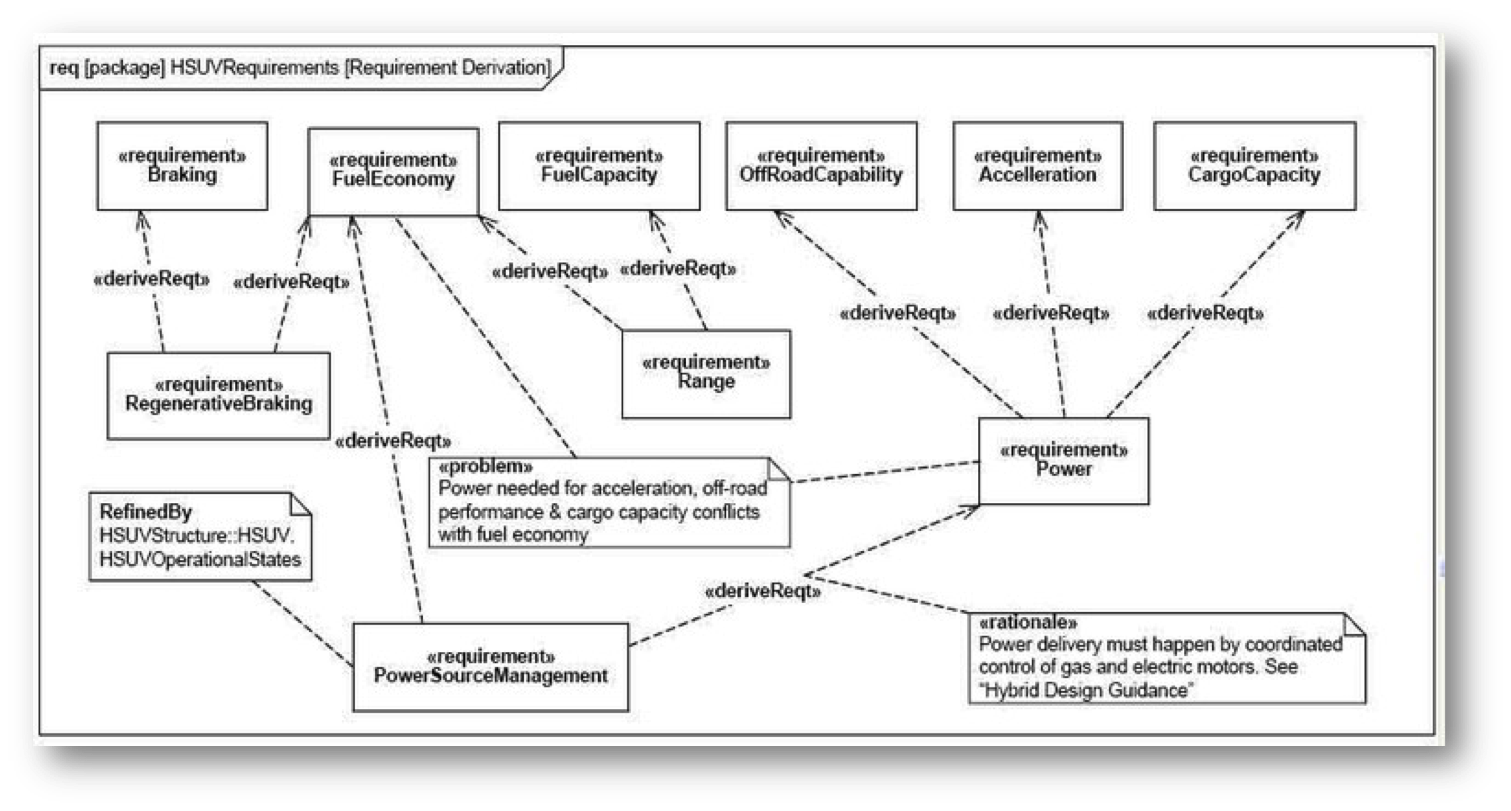
\includegraphics[scale=0.4]{images/hsuv-reqs2.png}}}}{images/hsuv-{}reqs2.png}
\end{center}
\caption{Exemples de dépendances entre exigences}
\end{figure}

\section{Les considérations sur la traçabilité}
\label{_les_considérations_sur_la_traçabilité}\hyperlabel{_les_considérations_sur_la_traçabilité}%

Une fois que les \emph{requirements} ont été définis et organisés, il est utile de les lier au moins aux \emph{use cases} (en utilisant \texttt{<{}<{}r\penalty5000 e\penalty5000 f\penalty5000 i\penalty5000 n\penalty5000 e>{}>{}} par exemple) et aux éléments structurels (en utilisant \texttt{<{}<{}s\penalty5000 a\penalty5000 t\penalty5000 i\penalty5000 s\penalty5000 f\penalty5000 y>{}>{}} par exemple), mais ceci
sera abordé dans la partie \hyperlink{transvers}{transverse}.
\begin{DBKadmonition}{images/icons/note.png}{Note}

En général chaque \emph{requirement} devrait être relié à au moins un \emph{use case} (et vice-{}versa!).
\end{DBKadmonition}

\section{Annotations des \emph{Requirements}}
\label{_annotations_des_emphasis_requirements_emphasis}\hyperlabel{_annotations_des_emphasis_requirements_emphasis}%

Il est possible d’annoter les éléments de modélisation en précisant les raisons
(\emph{rationale}) ou les éventuels problèmes anticipés (\emph{problem}).
\begin{figure}[H]

\begin{center}
\imgexists{images/hsuv-reqs2.png}{{\imgevalsize{images/hsuv-reqs2.png}{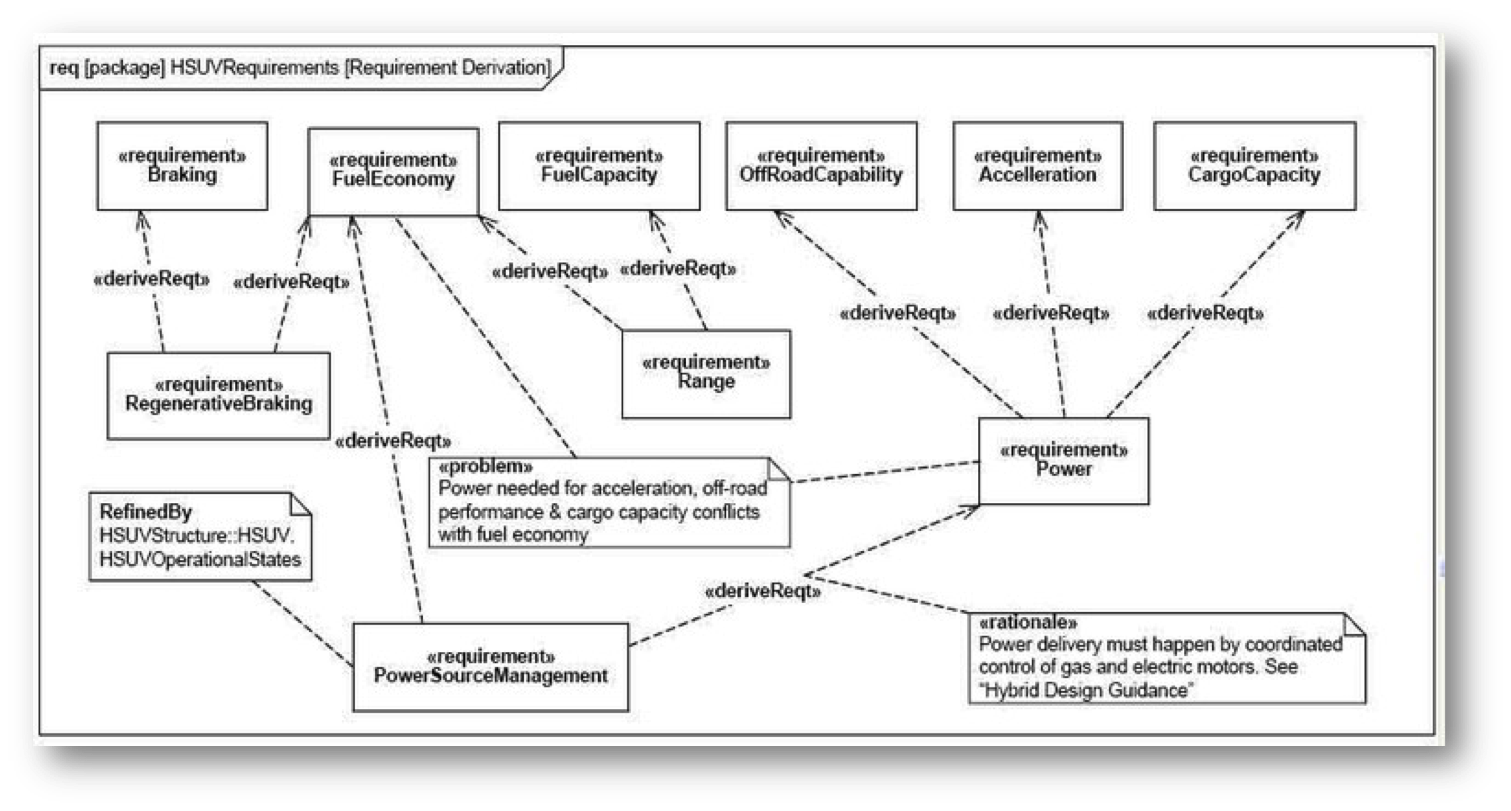
\includegraphics[scale=0.5]{images/hsuv-reqs2.png}}}}{images/hsuv-{}reqs2.png}
\end{center}
\caption{Exemples de \emph{rationale} et \emph{problem}}
\end{figure}

\section{Les \emph{Use Case Diagrams} (scénarios)}
\label{_les_emphasis_use_case_diagrams_emphasis_scénarios}\hyperlabel{_les_emphasis_use_case_diagrams_emphasis_scénarios}%

Bien que nous traitions les cas d’utilisation dans la partie \hyperlink{behavior}{comportement}, nous les abordons
        ici du fait de leur proximité avec les \emph{requirements}.
\begin{figure}[H]

\begin{center}
\imgexists{images/req-uc-relation.png}{{\imgevalsize{images/req-uc-relation.png}{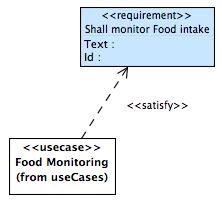
\includegraphics[scale=0.5]{images/req-uc-relation.png}}}}{images/req-{}uc-{}relation.png}
\end{center}
\caption{Exemple de lien entre \emph{use case} et \emph{requirements}}
\end{figure}

Ce diagramme est exactement identique à celui d’\href{http://www.uml.org/}{UML}\index{UML}.
\begin{figure}[H]

\begin{center}
\imgexists{images/UCGestionNotes.png}{{\imgevalsize{images/UCGestionNotes.png}{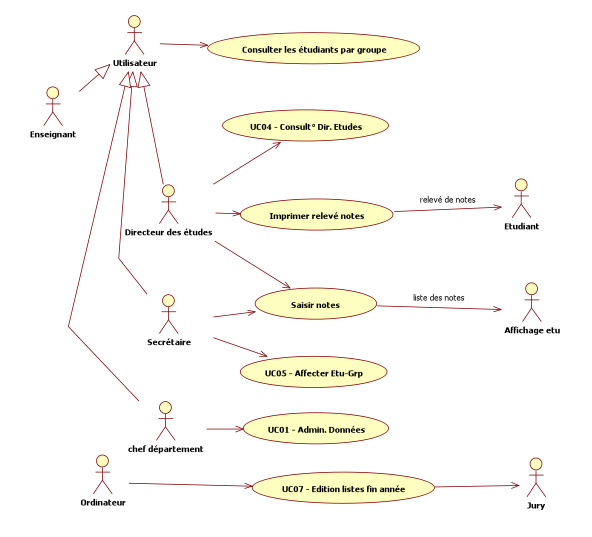
\includegraphics[scale=0.5]{images/UCGestionNotes.png}}}}{images/UCGestionNotes.png}
\end{center}
\caption{Exemple de diagrammes des cas d’utilisation}
\end{figure}
\begin{figure}[H]

\begin{center}
\imgexists{images/uc.png}{{\imgevalsize{images/uc.png}{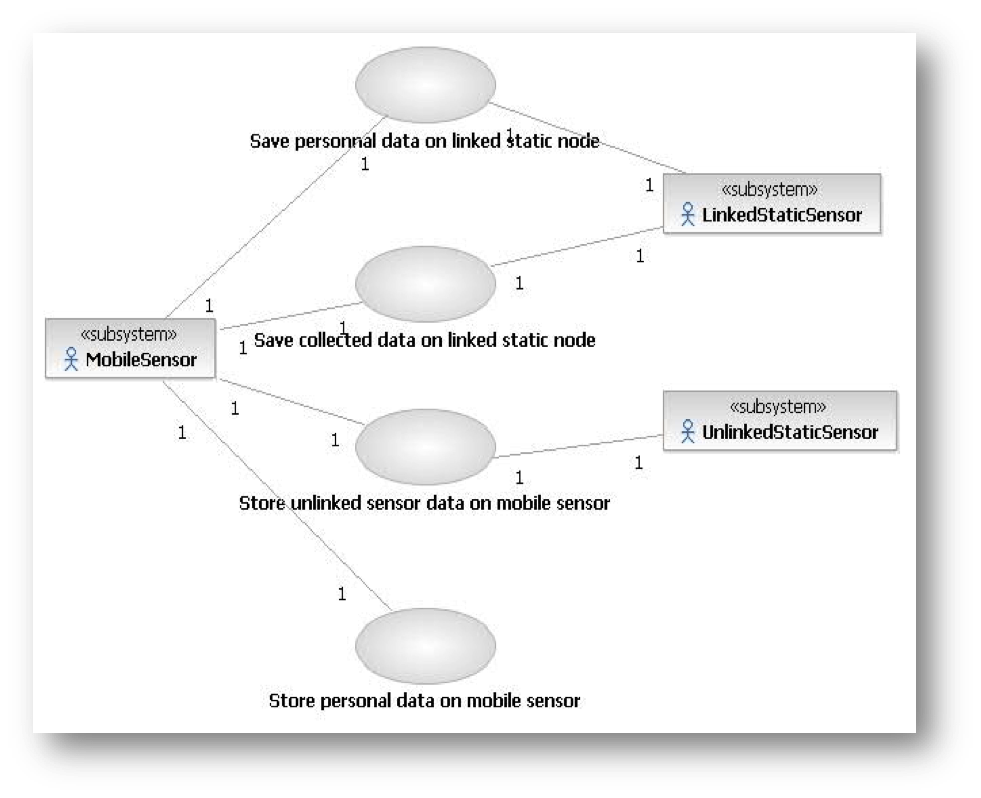
\includegraphics[scale=0.6]{images/uc.png}}}}{images/uc.png}
\end{center}
\caption{Autre exemple de diagrammes des cas d’utilisation}
\end{figure}
\begin{DBKadmonition}{images/icons/tip.png}{ASTUCE}

Un acteur représente un rôle joué par un utilisateur humain. Il faut donc plutôt raisonner sur les rôles que sur les personnes elles-{}mêmes pour identifier les acteurs.
\end{DBKadmonition}

\section{En résumé}
\label{_en_résumé_2}\hyperlabel{_en_résumé_2}%

Les exigences sont très importantes en ingénierie système, plus en tout cas qu’en ingénierie logiciel,
du fait de la multiplication des sous-{}systèmes et donc des intermédiaires (fournisseurs, sous-{}traitants, etc.)
avec qui les aspects contractuels seront souvent basés sur ces exigences. Il n’est donc pas étonnant qu’un  diagramme
et des mécanismes dédiés aient été prévus en \href{http://www.omgwiki.org/OMGSysML/}{SysML}\index{SysML}.
\begin{center}
\begingroup%
\setlength{\newtblsparewidth}{\linewidth-2\tabcolsep-2\tabcolsep-2\tabcolsep-2\tabcolsep-2\tabcolsep-2\tabcolsep}%
\setlength{\newtblstarfactor}{\newtblsparewidth / \real{97}}%

\begin{longtable}{lllll}\caption[{Déclinaison des Exigences}]{Déclinaison des Exigences}\tabularnewline
\hline
\multicolumn{1}{|p{16\newtblstarfactor}|}{\raggedright\bfseries%
%
 %
}&\multicolumn{1}{p{33\newtblstarfactor}|}{\raggedright\bfseries%
%
 \textbf{Requirements} %
}&\multicolumn{1}{p{16\newtblstarfactor}|}{\raggedright\bfseries%
%
 Structure   %
}&\multicolumn{1}{p{16\newtblstarfactor}|}{\raggedright\bfseries%
%
 Comportement    %
}&\multicolumn{1}{p{16\newtblstarfactor}|}{\raggedright\bfseries%
%
 Transverse%
}\tabularnewline
\cline{1-1}\cline{2-2}\cline{3-3}\cline{4-4}\cline{5-5}\endfirsthead
\caption[]{(continued)}\tabularnewline
\hline
\multicolumn{1}{|p{16\newtblstarfactor}|}{\raggedright\bfseries%
%
 %
}&\multicolumn{1}{p{33\newtblstarfactor}|}{\raggedright\bfseries%
%
 \textbf{Requirements} %
}&\multicolumn{1}{p{16\newtblstarfactor}|}{\raggedright\bfseries%
%
 Structure   %
}&\multicolumn{1}{p{16\newtblstarfactor}|}{\raggedright\bfseries%
%
 Comportement    %
}&\multicolumn{1}{p{16\newtblstarfactor}|}{\raggedright\bfseries%
%
 Transverse%
}\tabularnewline
\cline{1-1}\cline{2-2}\cline{3-3}\cline{4-4}\cline{5-5}\endhead
\multicolumn{1}{|p{16\newtblstarfactor}|}{\raggedright%
\textbf{Organisation}
%
}&\multicolumn{1}{p{33\newtblstarfactor}|}{\raggedright%
\texttt{⊕–}, \texttt{<{}<{}d\penalty5000 e\penalty5000 r\penalty5000 i\penalty5000 v\penalty5000 e\penalty5000 R\penalty5000 e\penalty5000 q\penalty5000 t>{}>{}}
%
}&\multicolumn{1}{p{16\newtblstarfactor}|}{\raggedright%
%
}&\multicolumn{1}{p{16\newtblstarfactor}|}{\raggedright%
%
}&\multicolumn{1}{p{16\newtblstarfactor}|}{\raggedright%
%
}\tabularnewline
\cline{1-1}\cline{2-2}\cline{3-3}\cline{4-4}\cline{5-5}\multicolumn{1}{|p{16\newtblstarfactor}|}{\raggedright%
\textbf{Analyse}
%
}&\multicolumn{1}{p{33\newtblstarfactor}|}{\raggedright%
\texttt{<{}<{}s\penalty5000 a\penalty5000 t\penalty5000 i\penalty5000 s\penalty5000 f\penalty5000 y>{}>{}}, \texttt{<{}<{}r\penalty5000 e\penalty5000 f\penalty5000 i\penalty5000 n\penalty5000 e>{}>{}}
%
}&\multicolumn{1}{p{16\newtblstarfactor}|}{\raggedright%
\texttt{<{}<{}s\penalty5000 a\penalty5000 t\penalty5000 i\penalty5000 s\penalty5000 f\penalty5000 y>{}>{}} entre reqs et UC
%
}&\multicolumn{1}{p{16\newtblstarfactor}|}{\raggedright%
\texttt{<{}<{}r\penalty5000 e\penalty5000 f\penalty5000 i\penalty5000 n\penalty5000 e>{}>{}}
%
}&\multicolumn{1}{p{16\newtblstarfactor}|}{\raggedright%
%
}\tabularnewline
\cline{1-1}\cline{2-2}\cline{3-3}\cline{4-4}\cline{5-5}\multicolumn{1}{|p{16\newtblstarfactor}|}{\raggedright%
\textbf{Conception}
%
}&\multicolumn{1}{p{33\newtblstarfactor}|}{\raggedright%
\texttt{<{}<{}a\penalty5000 l\penalty5000 l\penalty5000 o\penalty5000 c\penalty5000 a\penalty5000 t\penalty5000 e>{}>{}}
%
}&\multicolumn{1}{p{16\newtblstarfactor}|}{\raggedright%
%
}&\multicolumn{1}{p{16\newtblstarfactor}|}{\raggedright%
%
}&\multicolumn{1}{p{16\newtblstarfactor}|}{\raggedright%
%
}\tabularnewline
\cline{1-1}\cline{2-2}\cline{3-3}\cline{4-4}\cline{5-5}\multicolumn{1}{|p{16\newtblstarfactor}|}{\raggedright%
\textbf{Implémentation}
%
}&\multicolumn{1}{p{33\newtblstarfactor}|}{\raggedright%
\texttt{<{}<{}s\penalty5000 a\penalty5000 t\penalty5000 i\penalty5000 s\penalty5000 f\penalty5000 y>{}>{}}, \texttt{<{}<{}v\penalty5000 e\penalty5000 r\penalty5000 i\penalty5000 f\penalty5000 y>{}>{}}
%
}&\multicolumn{1}{p{16\newtblstarfactor}|}{\raggedright%
%
}&\multicolumn{1}{p{16\newtblstarfactor}|}{\raggedright%
%
}&\multicolumn{1}{p{16\newtblstarfactor}|}{\raggedright%
%
}\tabularnewline
\hline
\end{longtable}\endgroup%

\end{center}

En terme de démarche, il est classique d’avoir de nombreux aller-{}retour entre la modélisation
des exigences et la modélisation du système lui-{}même (cf. Figure \ref{sysmod}).
\begin{figure}[H]

\begin{center}
\imgexists{images/zigzag.png}{{\imgevalsize{images/zigzag.png}{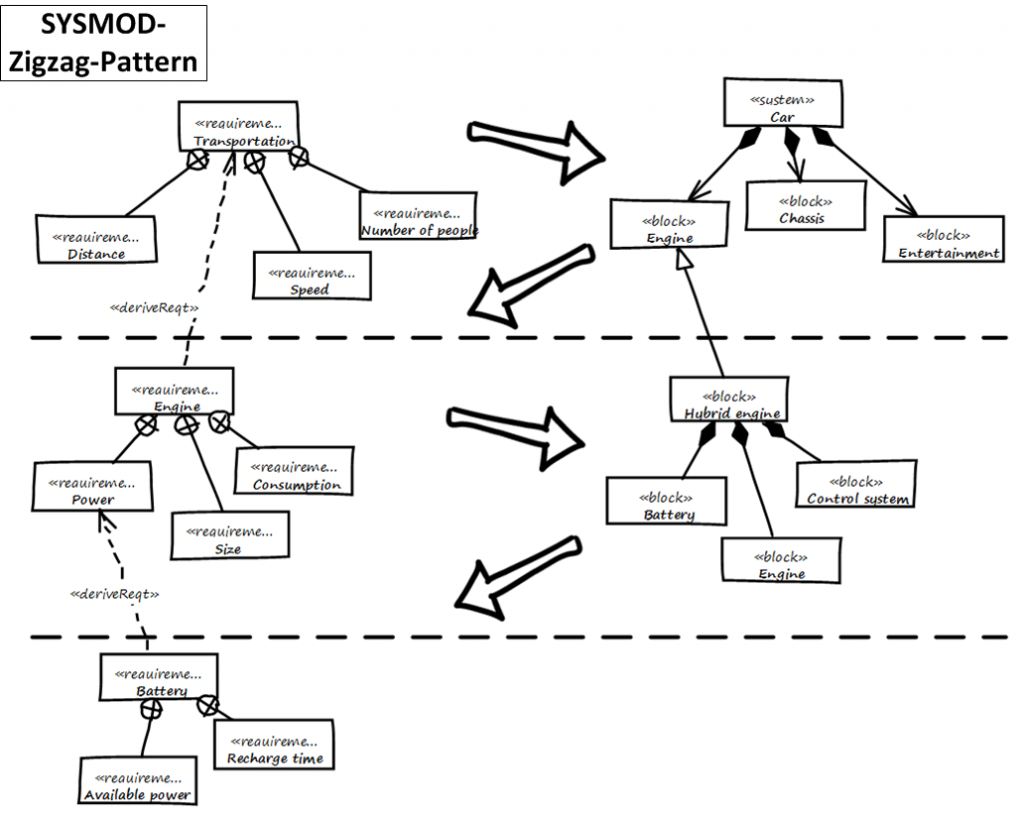
\includegraphics[scale=0.3]{images/zigzag.png}}}}{images/zigzag.png}
\end{center}
\caption{Exemple de démarche (\emph{SYSMOD Zigzag pattern})}
\label{sysmod}\hyperlabel{sysmod}%
\end{figure}

\section{Questions de révision}
\label{_questions_de_révision_2}\hyperlabel{_questions_de_révision_2}%
\begin{itemize}

\item{} Quelles sont les différences entre \textbf{besoins} et \textbf{exigences} ?



\item{} En quoi les cas d’utilisation sont-{}ils complémentaires des exigences?

\begin{enumerate}[label=\arabic*.]

\item{} Quelle est la différence entre un \emph{package} de type \textbf{\emph{model}} et un \emph{package} de type \textbf{\emph{package}}?


\end{enumerate}

\end{itemize}

% ------- 
% Chapter 
% ------- 

\chapter{L’architecture du système}
\label{archi}\hyperlabel{archi}%

\section{Fondements}
\label{_fondements_3}\hyperlabel{_fondements_3}%

On abordera :
\begin{itemize}

\item{} l’organisation du système et des modèles



\item{} les \emph{Block Definition Diagrams} 


\item{} les \emph{Internal Block Diagrams} 


\item{} les \emph{Parametric Diagrams} (pour les contraintes physiques)



\item{} les \emph{Sequence Diagrams} (diagramme de séquence système)


\end{itemize}

\section{Organisation du système et des modèles}
\label{_organisation_du_système_et_des_modèles}\hyperlabel{_organisation_du_système_et_des_modèles}%

En terme d’organisation, le mécanisme clef est celui de \emph{package}.
Celui-{}ci va permettre d’organiser les modèles, pas le système lui-{}même.
Nous avons abordé cette organisation \hyperlink{package}{ici}.

Pour l’organisation du système, on trouve le plus souvent :
\begin{itemize}

\item{} un diagramme décrivant le contexte (le système dans son environnement), décrit dans un \emph{block definition diagram} (cf. Figure \ref{contextebdd})



\item{} un diagramme décrivant les éléments internes principaux du système,  décrit dans un \emph{internal block diagram} 

\end{itemize}

\section{\emph{Block Definition Diagrams}}
\label{bddsec}\hyperlabel{bddsec}%

\subsection{Principes de base}
\label{_principes_de_base_2}\hyperlabel{_principes_de_base_2}%

Un \texttt{bdd} peut représenter :
\begin{itemize}

\item{} un \emph{package} 


\item{} un bloc



\item{} un bloc de contrainte (\emph{constraint block})


\end{itemize}

Un diagramme de bloc décrit les relations entre les blocs (composition, généralisations, …).
Ce diagramme utilise les mêmes éléments que le diagramme de classe \href{http://www.uml.org/}{UML}\index{UML}.
\begin{figure}[H]

\begin{center}
\imgexists{images/pacemaker-context.png}{{\imgevalsize{images/pacemaker-context.png}{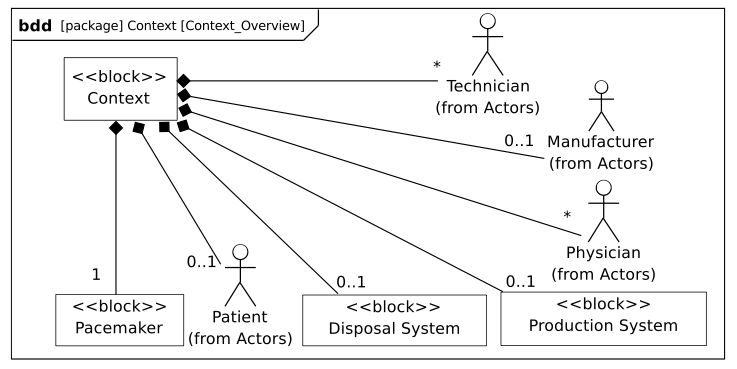
\includegraphics[scale=0.6]{images/pacemaker-context.png}}}}{images/pacemaker-{}context.png}
\end{center}
\caption{bdd du système dans son environnement}
\label{contextebdd}\hyperlabel{contextebdd}%
\end{figure}

Un bloc est constitué d’un certain nombre de compartiments (\emph{Compartments}) :

\noindent
\begin{description}
\item[{ \emph{Properties} }] \hspace{0em}\\
         Equivalent \href{http://www.uml.org/}{UML}\index{UML} des propriétés (e.g., attributs)

\item[{ \emph{Operations} }] \hspace{0em}\\
         Les méthodes supportées par les instances du bloc.

\item[{ \emph{Constraints} }] \hspace{0em}\\
         Les contraintes

\item[{ \emph{Allocations} }] \hspace{0em}\\
         Les allocations

\item[{ \emph{Requirements} }] \hspace{0em}\\
         Les exigences liées à ce bloc.

\item[{ \emph{User defined} }] \hspace{0em}\\
         On peut définir ses propres compartiments

\end{description}
\begin{figure}[H]

\begin{center}
\imgexists{images/constraints.png}{{\imgevalsize{images/constraints.png}{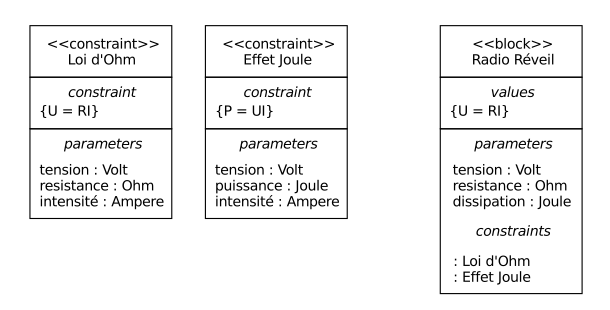
\includegraphics[scale=0.6]{images/constraints.png}}}}{images/constraints.png}
\end{center}
\caption{Exemple de définition de contraintes}
\end{figure}

\subsection{Propriétés}
\label{_propriétés}\hyperlabel{_propriétés}%

On peut différencier 3 types de propriétés d’un bloc :

\noindent
\begin{description}
\item[{ \emph{values} }] \hspace{0em}\\
         Des caractéristiques (quantifiables)

\item[{ \emph{parts} }] \hspace{0em}\\
         Les éléments qui composent le bloc (cf. Section \ref{ibd})

\item[{ \emph{references} }] \hspace{0em}\\
         Les éléments auquel le bloc a accès (via des associations ou des agrégations)

\end{description}
\begin{DBKadmonition}{images/icons/note.png}{Note}

Les \emph{values} sont ce qui se rapproche le plus des attributs de classes UML.
\end{DBKadmonition}

\subsection{\emph{Value Types}}
\label{_emphasis_value_types_emphasis}\hyperlabel{_emphasis_value_types_emphasis}%

Pour associer un type aux valeurs, \href{http://www.omgwiki.org/OMGSysML/}{SysML}\index{SysML} propose de définir des \emph{Value Types}.
\begin{figure}[H]

\begin{center}
\imgexists{images/valueType.png}{{\imgevalsize{images/valueType.png}{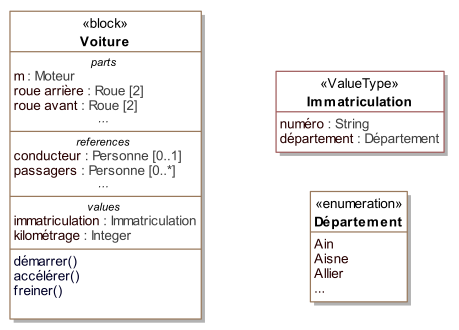
\includegraphics[scale=0.6]{images/valueType.png}}}}{images/valueType.png}
\end{center}
\caption{Définition de \emph{Value Types}.}
\end{figure}

\subsection{Associations entre blocs}
\label{_associations_entre_blocs}\hyperlabel{_associations_entre_blocs}%

Il existe deux types de relations entre blocs :
\begin{itemize}

\item{} l’association (y compris l’agrégation et la composition)



\item{} la généralisation/spécialisation


\end{itemize}

Ces deux types de relations, bien connues en \href{http://www.uml.org/}{UML}\index{UML}, permettent de matérialiser les liens qui existent entre les éléments du système. Avant d’aborder les associations, il est important de différencier la description d'éléments structurels sous la forme d’un bloc (au travers d’un \texttt{bdd} par exemple) et ces éléments pris individuellement. Ces derniers sont des \textbf{instances} individuelles du même bloc. Cette notion, très présente dans les approches orientées objets est souvent plus ardue à appréhender pour les ingénieurs systèmes. Il faut bien comprendre que la modélisation d’un bloc consiste à représenter l’ensemble des éléments qui caractérisent tout une série d’objets (des moteurs, des pompes, des données, etc.). Il serait fastidieux de les représenter tous (individuellement), et c’est donc leur "signature" que l’on représente. C’est pour cela qu’un bloc n’est pas un élément physique, mais simplement sa représentation, tandis qu’une instance de ce bloc représentera elle cet élément physique. C’est le cas notamment des participants d’un diagramme de séquence ou encore des parties d’un composé, qui sont des instances et non des blocs.

\subsubsection{Association}
\label{_association}\hyperlabel{_association}%

Une \textbf{association} est un ensemble de liens permanents existant entre les instances de deux ou plusieurs blocs.
On dira qu’une association lie plusieurs blocs ou que les blocs \textbf{participent} à l’association.

Une association possède plusieurs propriétés :

\noindent
\begin{description}
\item[{ Dimension d’une association
}] \hspace{0em}\\
 Nombre de blocs mis en jeu par l’association\newline
 (binaire : 2, ternaire : 3, n-{}aire : n)\newline
 
\end{description}
\begin{DBKadmonition}{images/icons/note.png}{Exemple d’association binaire}

Soient les bloc \texttt{Fou\penalty5000 r\penalty5000 n\penalty5000 i\penalty5000 s\penalty5000 s\penalty5000 e\penalty5000 urs} et \texttt{Pro\penalty5000 d\penalty5000 u\penalty5000 its}.
On veut indiquer quels sont les produits susceptibles d’être fournis par chaque fournisseur et quels sont les fournisseurs susceptibles de fournir chaque produit.

\noindent\imgexists{/Users/bruel/dev/asciidoc/ACSI/images/prod-fourn.png}{{\imgevalsize{/Users/bruel/dev/asciidoc/ACSI/images/prod-fourn.png}{\includegraphics[scale=0.4]{/Users/bruel/dev/asciidoc/ACSI/images/prod-fourn.png}}}}{/Users/bruel/dev/asciidoc/ACSI/images/prod-{}fourn.png}
\end{DBKadmonition}

\noindent
\begin{description}
\item[{ Nom d’une association
}] \hspace{0em}\\
 Afin de clarifier les informations, il est important de nommer les associations.\newline
 Il existe trois façons de nommer une association :

\begin{itemize}

\item{} un verbe à l’infinitif (e.g., \texttt{Fou\penalty5000 r\penalty5000 nir})



\item{} un verbe conjugué avec un sens de lecture : \texttt{Fou\penalty5000 r\penalty5000 n\penalty5000 i\penalty5000 t >{}}  ou  \texttt{<{} E\penalty5000 s\penalty5000 t f\penalty5000 o\penalty5000 u\penalty5000 r\penalty5000 n\penalty5000 i par} 


\item{} un rôle (placé à une extrémité de l’association)


\end{itemize}
\item[{ Cardinalité
}] \hspace{0em}\\
 Indique à combien d’instances minimum et maximum du bloc d’en face est lié toute instance du bloc de départ. Elle est représentée par un couple \texttt{(M.\penalty0 .\penalty0 N)}.

\end{description}
\begin{DBKadmonition}{images/icons/note.png}{Note}

Attention, dans une cardinalité \texttt{M.\penalty0 .\penalty0 N}, \texttt{M} doit toujours être inférieur ou égal à \texttt{N}.  Exemple : \texttt{3.\penalty0 .\penalty0 10}.
\end{DBKadmonition}

\subsubsection{Vers le code : que signifie vraiment une association?}
\label{_vers_le_code_que_signifie_vraiment_une_association}\hyperlabel{_vers_le_code_que_signifie_vraiment_une_association}%

En terme de logiciel, une \textbf{association} représente une contrainte sur la suite du développement : que ce soit un \textbf{code} (en langage orienté objet la plupart du temps) ou une \textbf{base de donnée}.

Pour reprendre l’exemple précédent, cela signifie concrètement au niveau d’un code par exemple
que depuis une variable \texttt{Pro\penalty5000 d\penalty5000 u\penalty5000 its} on doit être capable d’accéder à une variable (correspondante)
de type tableau (ou liste, ou …) de \texttt{Fou\penalty5000 r\penalty5000 n\penalty5000 i\penalty5000 s\penalty5000 s\penalty5000 e\penalty5000 urs}.

Ce qui peut donner en java :

\begin{lstlisting}[language=java,firstnumber=1,]
public class Produits
{
//Produits Attributes
private String idPro;
private String designation;
private float poids;

//Produits Associations
private List<Fournisseurs> fournisseurs;
...
\end{lstlisting}

En terme d’ingénierie système, on utilisera plutôt des associations spécifiques (l’agrégation et la composition).
\begin{figure}[H]

\begin{center}
\imgexists{/Users/bruel/dev/asciidoc/ACSI/images/aggreg-comp.png}{{\imgevalsize{/Users/bruel/dev/asciidoc/ACSI/images/aggreg-comp.png}{\includegraphics[scale=0.5]{/Users/bruel/dev/asciidoc/ACSI/images/aggreg-comp.png}}}}{/Users/bruel/dev/asciidoc/ACSI/images/aggreg-{}comp.png}
\end{center}
\caption{Deux façon de représenter une propriété de type \texttt{B}}
\end{figure}

En terme d’Ingénierie Système \index{IS}, une composition indique que l'élément est une partie intégrante (on parle de \emph{part}) du tout (un composant, comme le moteur d’une voiture par exemple) tandis q’une agrégation indique que l'élément est une partie "externe" (on parle de \emph{reference}) comme la batterie d’un portable.
\begin{DBKadmonition}{images/icons/note.png}{Note}

Un moyen simple en terme logiciel de déterminer si une association \texttt{A→B} est une association dirigée (navigable dans un sens), une agrégation ou une composition est de raisonner en terme d’implémentation :
\begin{itemize}

\item{} c’est une agrégation si \texttt{b} est initialisé dans le constructeur de \texttt{A} ;



\item{} c’est une composition si il est aussi détruit dans le destructeur de \texttt{A} ;



\item{} c’est une association dirigée simple si aucun des deux cas précédent ne s’applique.


\end{itemize}
\end{DBKadmonition}

\subsubsection{Généralisation/spécialisation}
\label{_généralisation_spécialisation}\hyperlabel{_généralisation_spécialisation}%

Lorsque plusieurs blocs ont des caractéristiques en communs (propriétés, associations, comportement), il peut être utile de "factoriser" ces éléments en un bloc dont les autres vont "hériter". Quand on réalise ces liens hiérarchiques (on utilise souvent le terme "est un") en partant des blocs différents pour établir un nouveau bloc contenant les points communs on parle de \textbf{généralisation}. À l’inverse, quand on constate qu’un bloc possède réellement plusieurs déclinaisons différentes et que l’on créé alors des blocs spécifiques, on parle alors de \textbf{spécialisation}.
\begin{figure}[H]

\begin{center}
\imgexists{images/genspec.png}{{\imgevalsize{images/genspec.png}{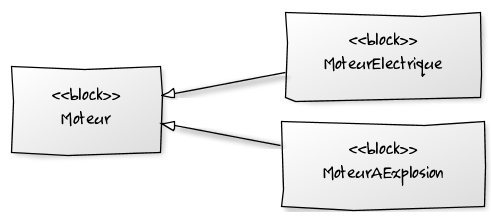
\includegraphics[scale=0.5]{images/genspec.png}}}}{images/genspec.png}
\end{center}
\caption{Exemple de lien de généralisation/spécialisation}
\end{figure}

On retrouve cette association entre blocs, mais aussi entre acteurs, cas d’utilisation, etc.

\section{\emph{Internal Block Diagrams}}
\label{ibd}\hyperlabel{ibd}%

Un \texttt{ibd} décrit la structure interne d’un bloc sous forme de :

\noindent
\begin{description}
\item[{ parts
}] \hspace{0em}\\
         Les parties qui constituent le système (ses sous-{}systèmes)

\item[{ ports
}] \hspace{0em}\\
         Elément d’interaction avec un bloc

\item[{ connecteurs
}] \hspace{0em}\\
         Liens entre ports

\end{description}

\subsection{Parts}
\label{_parts}\hyperlabel{_parts}%

Les parties sont représentés par les éléments au bout d’une composition dans un \texttt{bdd}.
Elles sont créés à la création du bloc qui les contient et sont détruites avec lui s’il
est détruit (dépendance de vie).
\begin{DBKadmonition}{images/icons/warning.png}{AVERTISSEMENT}

Il ne s’agit pas de redessiner le BDD. Les \emph{parts} sont des instances et non des classes (au sens objet).\newline
 Cela ne pose aucun problème à un ingénieur système, mais ça peut en poser à un ingénieur logiciel.
\end{DBKadmonition}

On représente les \emph{parts} comme des bloc en traits pleins
et les \emph{references} comme des blocs en trait pointillés.
\begin{figure}[H]

\begin{center}
\imgexists{images/parts.png}{{\imgevalsize{images/parts.png}{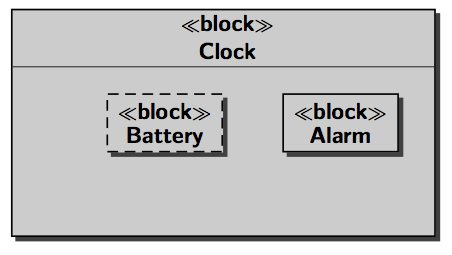
\includegraphics[scale=0.4]{images/parts.png}}}}{images/parts.png}
\end{center}
\caption{Exemple de \emph{Parts}}
\end{figure}
\begin{figure}[H]

\begin{center}
\imgexists{images/parts2.png}{{\imgevalsize{images/parts2.png}{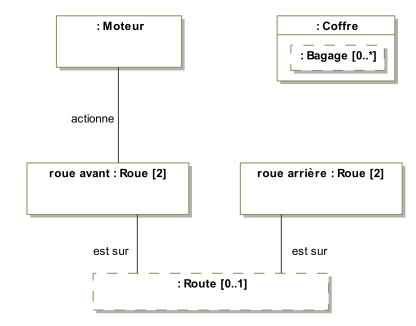
\includegraphics[scale=0.4]{images/parts2.png}}}}{images/parts2.png}
\end{center}
\caption{Autre exemple de \emph{Parts}}
\end{figure}

\subsection{Ports}
\label{_ports}\hyperlabel{_ports}%

Les ports :
\begin{itemize}

\item{} préservent l’encapsulation du bloc



\item{} matérialise le fait que les interactions avec l’extérieur (via un port)
sont transmise à une partie (via un connecteur)



\item{} les ports connectés doivent correspondre (\emph{kind}, \emph{type}, \emph{direction}, etc.)


\end{itemize}
\begin{DBKadmonition}{images/icons/note.png}{Note}

Les ports définissent les points d’interaction offerts (\texttt{«pr\penalty5000 o\penalty5000 v\penalty5000 i\penalty5000 d\penalty5000 ed»}) et requis (\texttt{«re\penalty5000 q\penalty5000 u\penalty5000 i\penalty5000 r\penalty5000 ed»}) entre les blocs.\newline
 Les connecteurs peuvent traverser les "frontières" sans exiger de ports à chaque hiérarchie.
\end{DBKadmonition}
\begin{figure}[H]

\begin{center}
\imgexists{images/ports-flots.png}{{\imgevalsize{images/ports-flots.png}{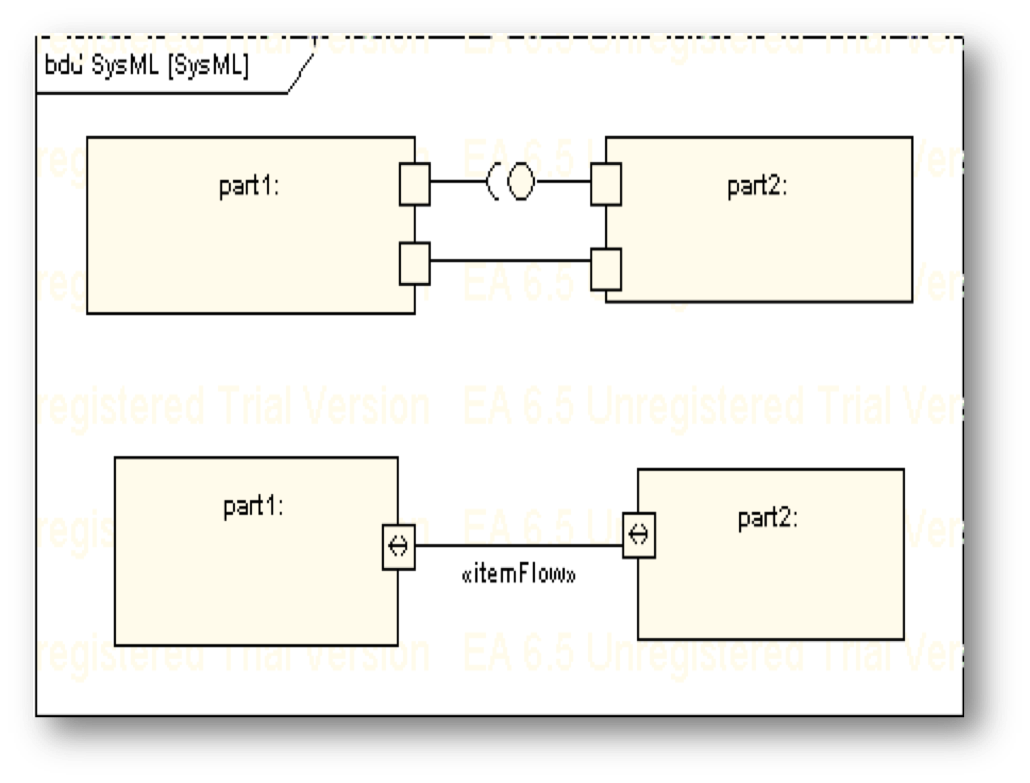
\includegraphics[scale=0.6]{images/ports-flots.png}}}}{images/ports-{}flots.png}
\end{center}
\caption{Exemples de flots}
\end{figure}
\begin{figure}[H]

\begin{center}
\imgexists{images/flots.png}{{\imgevalsize{images/flots.png}{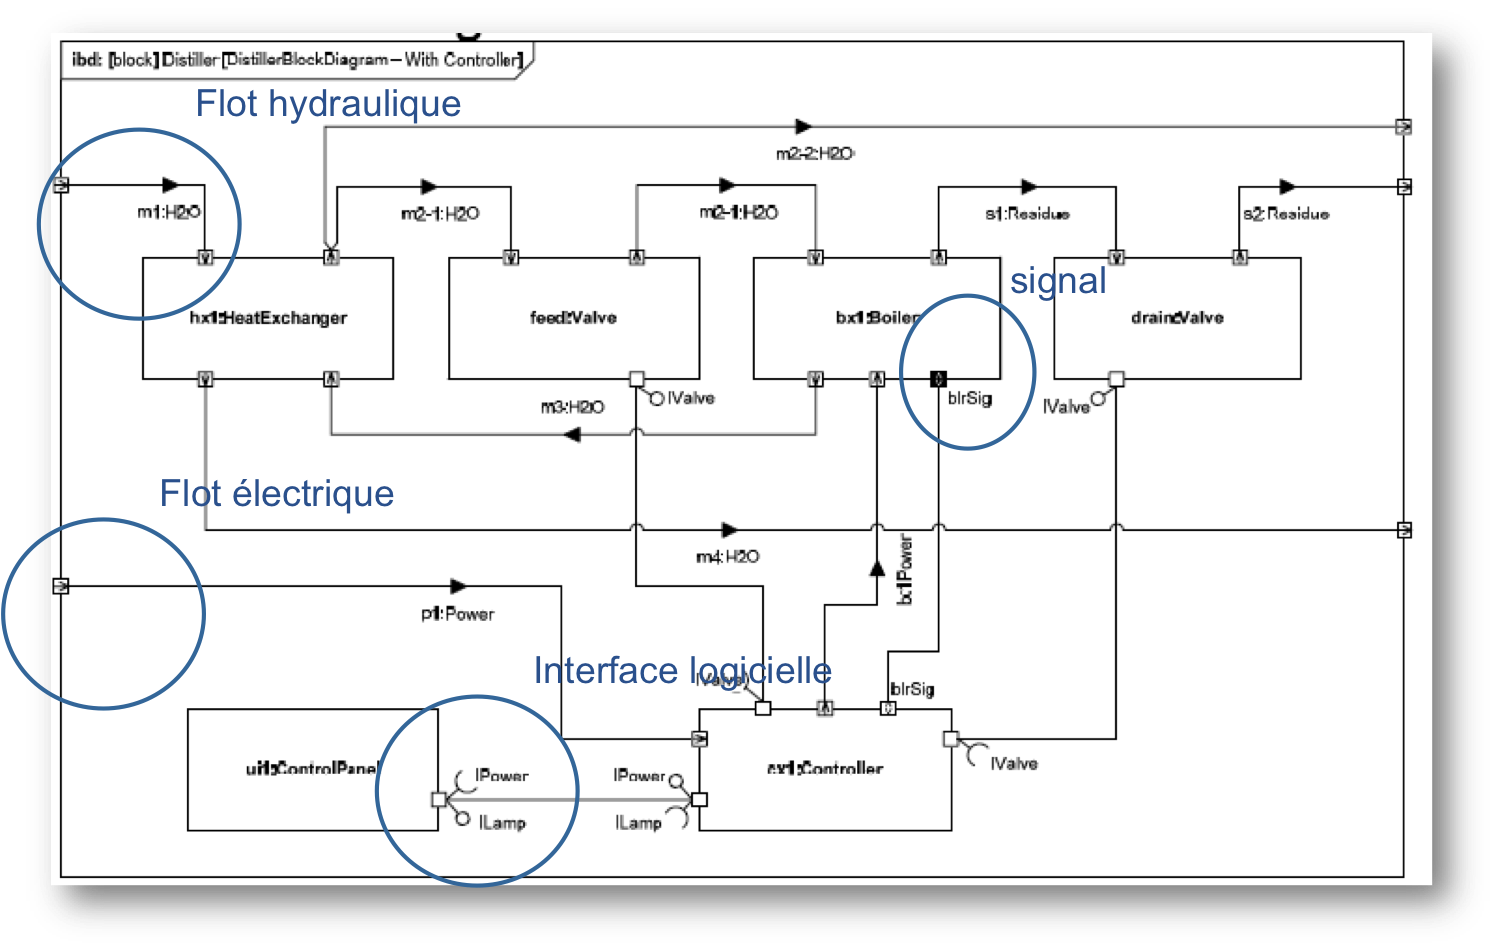
\includegraphics[scale=0.5]{images/flots.png}}}}{images/flots.png}
\end{center}
\caption{Exemples de flots multi-{}physique entre ports}
\end{figure}

Les ports peuvent être de nature classique (comme en \href{http://www.uml.org/}{UML}\index{UML}) et représenter la fourniture ou le besoin de services.
Ils peuvent aussi être de nature "flux physique".

Les \texttt{Flux} peuvent être :
\begin{itemize}

\item{} atomiques (un seul flux),



\item{} composites (agrégation de flux de natures différentes).


\end{itemize}
\begin{DBKadmonition}{images/icons/note.png}{Note}

Un \emph{flow port} atomique ne spécifie qu’un seul type de flux en entrée ou en sortie (ou les deux),
la direction étant simplement indiquée par une flèche à l’intérieur du carré représentant le port. Il peut être typé par un bloc ou un \emph{Value Type} représentant le type d’élément pouvant circuler en entrée ou en sortie du port.
\end{DBKadmonition}

\section{\emph{Parametric Diagrams}}
\label{param}\hyperlabel{param}%

Ce diagramme utilise 3 concepts clefs :
\begin{itemize}

\item{} \emph{Constraints} (un type de bloc)



\item{} \emph{Parametric diagram} (un type d'\texttt{ibd})



\item{} \emph{Value binding} 

\end{itemize}

\subsection{Contraintes}
\label{_contraintes}\hyperlabel{_contraintes}%

C’est un bloc particulier :
\begin{itemize}

\item{} avec un stéréotype \texttt{≪co\penalty5000 n\penalty5000 s\penalty5000 t\penalty5000 r\penalty5000 a\penalty5000 i\penalty5000 nt≫} (au lieu de bloc)



\item{} des paramètres en guise d’attributs



\item{} des relations liant (contraignant) ces paramètres


\end{itemize}
\begin{figure}[H]

\begin{center}
\imgexists{images/constraints.png}{{\imgevalsize{images/constraints.png}{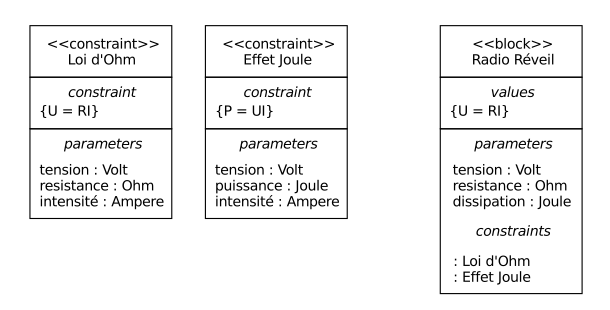
\includegraphics[scale=0.5]{images/constraints.png}}}}{images/constraints.png}
\end{center}
\caption{Exemple de contraintes}
\end{figure}

\subsection{Diagramme paramétrique}
\label{_diagramme_paramétrique}\hyperlabel{_diagramme_paramétrique}%

C’est une forme particulière de \emph{Internal Block Definition}
\begin{figure}[H]

\begin{center}
\imgexists{images/param.png}{{\imgevalsize{images/param.png}{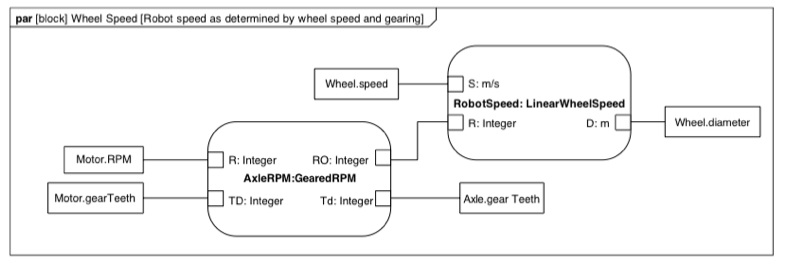
\includegraphics[scale=0.5]{images/param.png}}}}{images/param.png}
\end{center}
\caption{Exemple de diagramme paramétrique}
\end{figure}

\subsection{\emph{Value Binding}}
\label{_emphasis_value_binding_emphasis}\hyperlabel{_emphasis_value_binding_emphasis}%

Une fois les contraintes exprimées, il faut lier les paramètres (formels) à des valeurs (paramètre réel). C’est l’objet des \emph{Value Binding}.

Pour assigner des valeurs spécifiques, on utilise des \emph{Block Configurations};
\begin{figure}[H]

\begin{center}
\imgexists{images/blockconf.png}{{\imgevalsize{images/blockconf.png}{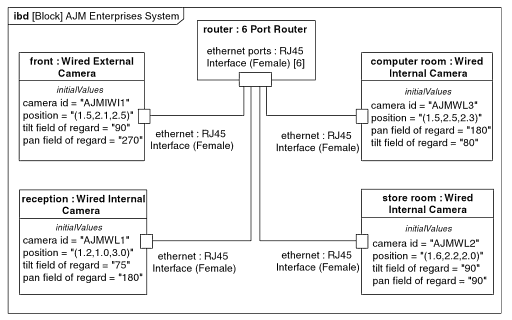
\includegraphics[scale=0.6]{images/blockconf.png}}}}{images/blockconf.png}
\end{center}
\caption{Exemple de bloc de configuration}
\end{figure}

\section{Diagrammes de séquence système}
\label{_diagrammes_de_séquence_système}\hyperlabel{_diagrammes_de_séquence_système}%

Les diagrammes de séquence système (DSS) sont des \emph{Sequence Diagrams} \href{http://www.uml.org/}{UML}\index{UML} classiques où seul le système est représenté comme une boîte noire en interaction avec son environnement (les utilisateurs généralement).

Il permet de décrire les scénarios des cas d’utilisation sans entrer dans les détails. Il convient donc mieux à l’ingénierie système qu’un diagramme de séquence classique (cf. section sur les Section \ref{seq}).
\begin{figure}[H]

\begin{center}
\imgexists{images/dss.png}{{\imgevalsize{images/dss.png}{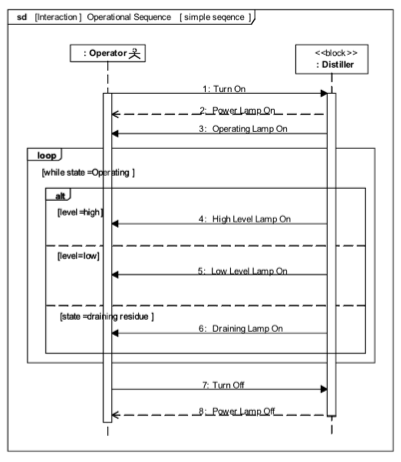
\includegraphics[scale=0.7]{images/dss.png}}}}{images/dss.png}
\end{center}
\caption{Exemples de DSS}
\end{figure}

\section{En résumé}
\label{_en_résumé_3}\hyperlabel{_en_résumé_3}%

En résumé, il existe plusieurs diagrammes permettant d’exprimer la structure du système à concevoir. En fonction du niveau de détail nécessaire on peut voir les sous-{}systèmes comme des boîtes noires (des blocs) ou comme des boîtes blanches (grâce à l'\texttt{ibd} correspondant).
\begin{center}
\begingroup%
\setlength{\newtblsparewidth}{\linewidth-2\tabcolsep-2\tabcolsep-2\tabcolsep-2\tabcolsep-2\tabcolsep-2\tabcolsep}%
\setlength{\newtblstarfactor}{\newtblsparewidth / \real{100}}%

\begin{longtable}{lllll}\caption[{Place des aspects structurels}]{Place des aspects structurels}\tabularnewline
\hline
\multicolumn{1}{|p{20\newtblstarfactor}|}{\raggedright\bfseries%
%
 %
}&\multicolumn{1}{p{20\newtblstarfactor}|}{\raggedright\bfseries%
%
 Requirements        %
}&\multicolumn{1}{p{20\newtblstarfactor}|}{\raggedright\bfseries%
%
 \textbf{Structure} %
}&\multicolumn{1}{p{20\newtblstarfactor}|}{\raggedright\bfseries%
%
 Comportement    %
}&\multicolumn{1}{p{20\newtblstarfactor}|}{\raggedright\bfseries%
%
 Transverse%
}\tabularnewline
\cline{1-1}\cline{2-2}\cline{3-3}\cline{4-4}\cline{5-5}\endfirsthead
\caption[]{(continued)}\tabularnewline
\hline
\multicolumn{1}{|p{20\newtblstarfactor}|}{\raggedright\bfseries%
%
 %
}&\multicolumn{1}{p{20\newtblstarfactor}|}{\raggedright\bfseries%
%
 Requirements        %
}&\multicolumn{1}{p{20\newtblstarfactor}|}{\raggedright\bfseries%
%
 \textbf{Structure} %
}&\multicolumn{1}{p{20\newtblstarfactor}|}{\raggedright\bfseries%
%
 Comportement    %
}&\multicolumn{1}{p{20\newtblstarfactor}|}{\raggedright\bfseries%
%
 Transverse%
}\tabularnewline
\cline{1-1}\cline{2-2}\cline{3-3}\cline{4-4}\cline{5-5}\endhead
\multicolumn{1}{|p{20\newtblstarfactor}|}{\raggedright%
\textbf{Organisation}
%
}&\multicolumn{1}{p{20\newtblstarfactor}|}{\raggedright%
%
}&\multicolumn{1}{p{20\newtblstarfactor}|}{\raggedright%
\texttt{pac\penalty5000 k\penalty5000 age}
%
}&\multicolumn{1}{p{20\newtblstarfactor}|}{\raggedright%
%
}&\multicolumn{1}{p{20\newtblstarfactor}|}{\raggedright%
%
}\tabularnewline
\cline{1-1}\cline{2-2}\cline{3-3}\cline{4-4}\cline{5-5}\multicolumn{1}{|p{20\newtblstarfactor}|}{\raggedright%
\textbf{Analyse}
%
}&\multicolumn{1}{p{20\newtblstarfactor}|}{\raggedright%
%
}&\multicolumn{1}{p{20\newtblstarfactor}|}{\raggedright%
\texttt{bdd} \texttt{par}
%
}&\multicolumn{1}{p{20\newtblstarfactor}|}{\raggedright%
%
}&\multicolumn{1}{p{20\newtblstarfactor}|}{\raggedright%
%
}\tabularnewline
\cline{1-1}\cline{2-2}\cline{3-3}\cline{4-4}\cline{5-5}\multicolumn{1}{|p{20\newtblstarfactor}|}{\raggedright%
\textbf{Conception}
%
}&\multicolumn{1}{p{20\newtblstarfactor}|}{\raggedright%
%
}&\multicolumn{1}{p{20\newtblstarfactor}|}{\raggedright%
\texttt{bdd} \texttt{par} \texttt{ibd} \texttt{dss}
%
}&\multicolumn{1}{p{20\newtblstarfactor}|}{\raggedright%
%
}&\multicolumn{1}{p{20\newtblstarfactor}|}{\raggedright%
%
}\tabularnewline
\cline{1-1}\cline{2-2}\cline{3-3}\cline{4-4}\cline{5-5}\multicolumn{1}{|p{20\newtblstarfactor}|}{\raggedright%
\textbf{Implémentation}
%
}&\multicolumn{1}{p{20\newtblstarfactor}|}{\raggedright%
%
}&\multicolumn{1}{p{20\newtblstarfactor}|}{\raggedright%
\texttt{bdd} \texttt{par} \texttt{ibd} \texttt{dss}
%
}&\multicolumn{1}{p{20\newtblstarfactor}|}{\raggedright%
%
}&\multicolumn{1}{p{20\newtblstarfactor}|}{\raggedright%
%
}\tabularnewline
\hline
\end{longtable}\endgroup%

\end{center}

\section{Questions de révision}
\label{_questions_de_révision_3}\hyperlabel{_questions_de_révision_3}%
\begin{enumerate}[label=\arabic*.]

\item{} Quelles sont les différences entre une association dirigée (\texttt{→}), une composition (losange noir) et l’agrégation (losange blanc) ?



\item{} Puisqu’un \texttt{bdd} me donne souvent la liste des sous-{}systèmes (liens de composition), pourquoi ai-{}je besoin d’un \texttt{ibd} ?


\end{enumerate}

% ------- 
% Chapter 
% ------- 

\chapter{Le comportement du système}
\label{_le_comportement_du_système}\hyperlabel{_le_comportement_du_système}%

\section{Fondements}
\label{behavior}\hyperlabel{behavior}%

On abordera :
\begin{itemize}

\item{} les \emph{Use Case Diagrams} (scénarios)



\item{} les \emph{Sequence Diagrams} 


\item{} les \emph{State Machines} 


\item{} les \emph{Activity Diagrams} 

\end{itemize}

\section{\emph{Use Case Diagrams}}
\label{usecase}\hyperlabel{usecase}%

Les éléments de base :

\noindent
\begin{description}
\item[{ Acteurs
}] \hspace{0em}\\
         les principaux acteurs (leur rôle) qui participent (on parle parfois d’acteurs principaux)
        ou qui bénéficient (on parle alors d’acteurs secondaires) du système.

\item[{ Cas d’utilisation
}] \hspace{0em}\\
         représente un ensemble d’actions réalisées par le système intéressant pour au moins un acteur

\item[{ Association
}] \hspace{0em}\\
         participation d’un acteur à un cas d’utilisation.

\item[{ Sujet
}] \hspace{0em}\\
         le domaine étudié (qui peut être une partie seulement de tout le système, pas forcément modélisé dans son ensemble)

\end{description}
\begin{DBKadmonition}{images/icons/tip.png}{ASTUCE}

Un acteur représente un rôle joué par un utilisateur humain. Il faut donc plutôt raisonner sur les rôles que sur les personnes elles-{}mêmes pour identifier les acteurs.
\end{DBKadmonition}

\section{Le Diagramme des Cas d’Utilisation}
\label{_le_diagramme_des_cas_d_utilisation}\hyperlabel{_le_diagramme_des_cas_d_utilisation}%

Le \textbf{Diagramme des Cas d’Utilisation} est un diagramme \href{http://www.uml.org/}{UML}\index{UML} permettant de représenter :
\begin{itemize}

\item{} les \textbf{UC} (\emph{Use Case} ou Cas d’Utilisation)



\item{} les \textbf{acteurs} (principaux et secondaires)



\item{} les \textbf{relations} 
\begin{itemize}

\item{} entre acteurs et \emph{Use Case} 


\item{} entre \emph{Use Cases} 

\end{itemize}

\end{itemize}
\begin{DBKadmonition}{images/icons/note.png}{Note}

On notera simplement \texttt{uc} pour signifier "diagramme des UC"
\end{DBKadmonition}

\subsection{Cas d’Utilisation (\emph{Use Case})}
\label{_cas_d_8217_utilisation_emphasis_use_case_emphasis}\hyperlabel{_cas_d_8217_utilisation_emphasis_use_case_emphasis}%

\label{uc}\hyperlabel{uc}%
Un cas d’utilisation représente un ensemble de \textbf{scénarios} que le système doit exécuter pour produire un résultat observable par un \hyperlink{acteur}{acteur}.

\subsubsection{Exemple de cas d’utilisation (UML)}
\label{_exemple_de_cas_d_8217_utilisation_uml}\hyperlabel{_exemple_de_cas_d_8217_utilisation_uml}%

Retrait par carte bancaire

\noindent
\begin{description}
\item[{ Scénario principal
}] \hspace{0em}\\
         L’UC démarre lorsque le Guichet Automatique Bancaire (GAB) demande au client son numéro confidentiel après l’introduction de sa CB. Le client
        entre son code et valide son entrée. Le GAB contrôle la validité du code. Si le code est valide, le GAB autorise
        le retrait et l’UC se termine.

\item[{ Scénario alternatif n°1 
}] \hspace{0em}\\
         Le client peut à tout instant annuler l’opération. La carte est éjectée et l’UC se termine.

\item[{ Exemple de codification de l’UC
}] \hspace{0em}\\
         UC01 ou RetraitCB (pour Retrait par carte bleue)

\end{description}

\subsubsection{Précisions}
\label{_précisions}\hyperlabel{_précisions}%

Un cas d’utilisation peut être précisé par :
\begin{itemize}

\item{} une description textuelle



\item{} un ou des diagrammes \href{http://www.uml.org/}{UML}\index{UML} (séquence, activité)


\end{itemize}
\begin{DBKadmonition}{images/icons/note.png}{Note}

Dans les outils, cette "précision" se manifeste par le fait que l’on "attache"
généralement un diagramme de séquence à un cas d’utilisation (clic droit sur un \emph{Use Case} → nouveau \texttt{seq}).
\end{DBKadmonition}

\subsection{Acteur}
\label{_acteur}\hyperlabel{_acteur}%

\label{acteur}\hyperlabel{acteur}%
Un acteur peut être une personne, un ensemble de personnes, un logiciel, un processus qui interagit avec un ou plusieurs \hyperlink{uc}{UC}.

On peut trouver plusieurs types d’acteurs :
\begin{itemize}

\item{} extérieurs au système (cf. \texttt{actor} Figure \ref{ucdiag})

\begin{itemize}

\item{} les acteurs principaux



\item{} les acteurs secondaires


\end{itemize}


\item{} exemples de types d’acteurs prédéfinis dans UML :

\begin{itemize}

\item{} \texttt{<{}<{}u\penalty5000 t\penalty5000 i\penalty5000 l\penalty5000 i\penalty5000 t\penalty5000 y>{}>{}} 


\item{} \texttt{<{}<{}p\penalty5000 r\penalty5000 o\penalty5000 c\penalty5000 e\penalty5000 s\penalty5000 s>{}>{}} 


\item{} \texttt{<{}<{}t\penalty5000 h\penalty5000 r\penalty5000 e\penalty5000 a\penalty5000 d>{}>{}} 

\end{itemize}

\end{itemize}
\begin{DBKadmonition}{images/icons/note.png}{Note}

On peut utiliser des liens de généralisation/spécialisation entre acteurs
pour représenter les possibilités pour le spécialisé d’avoir les mêmes
prérogatives (notamment en terme d’utilisation du système) que le généralisé.
\end{DBKadmonition}

\subsection{Relations entre acteurs et \emph{Use Case}}
\label{_relations_entre_acteurs_et_emphasis_use_case_emphasis}\hyperlabel{_relations_entre_acteurs_et_emphasis_use_case_emphasis}%

En général, une simple association relie acteurs et \emph{Use Case}.
On peut également orienter ces associations en plaçant une direction (flèche vide) au bout de l’association.

\subsection{Relations entre \emph{Use Case}}
\label{_relations_entre_emphasis_use_case_emphasis}\hyperlabel{_relations_entre_emphasis_use_case_emphasis}%

Après avoir lister les cas d’utilisation, il est utile de les organiser et de montrer les relations entre eux.
Plusieurs relations sont possibles :

\noindent
\begin{description}
\item[{ Extension (\texttt{<{}<{}e\penalty5000 x\penalty5000 t\penalty5000 e\penalty5000 n\penalty5000 d>{}>{}})
}] \hspace{0em}\\
         Indique que le \emph{Use Case} source est \textbf{éventuellement} exécutée en complément du \emph{Use Case} destination (cas particulier, erreur…). Le point précis où l’extension peut se produire est appelé \emph{extension point} (surtout utile quand il existe plusieurs extensions pour un même cas)

\item[{ Inclusion (\texttt{<{}<{}i\penalty5000 n\penalty5000 c\penalty5000 l\penalty5000 u\penalty5000 d\penalty5000 e>{}>{}})
}] \hspace{0em}\\
         Indique que le \emph{Use Case} est inclus \textbf{obligatoirement} dans un autre \emph{Use Case} (notion de sous-{}fonction par exemple)

\item[{ Généralisation
}] \hspace{0em}\\
         Relation entre un \emph{Use Case} général et un autre plus spécialisé qui hérite de ses caractéristiques et en rajoute (différents modes d’utilisation d’un système par exemple, ou encore différents acteurs impliqués)

\end{description}
\begin{figure}[H]

\begin{center}
\imgexists{/Users/bruel/dev/asciidoc/ACSI/dessins/UC.png}{{\imgevalsize{/Users/bruel/dev/asciidoc/ACSI/dessins/UC.png}{\includegraphics[scale=0.7]{/Users/bruel/dev/asciidoc/ACSI/dessins/UC.png}}}}{/Users/bruel/dev/asciidoc/ACSI/dessins/UC.png}
\end{center}
\caption{Notation dans le diagramme d’UC}
\label{ucdiag}\hyperlabel{ucdiag}%
\end{figure}
\begin{DBKadmonition}{images/icons/tip.png}{ASTUCE}

On n’utilise généralement \texttt{<{}<{}i\penalty5000 n\penalty5000 c\penalty5000 l\penalty5000 u\penalty5000 d\penalty5000 e>{}>{}} que dans le cas où le sous-{}cas d’utilisation est
inclut dans plusieurs UC. Si ce n’est pas le cas, il est généralement englobé dans l’UC.
\end{DBKadmonition}

\subsection{Pour construire un UC (de manière générale)}
\label{_pour_construire_un_uc_de_manière_générale}\hyperlabel{_pour_construire_un_uc_de_manière_générale}%
\begin{enumerate}[label=\arabic*.]

\item{} identifier les acteurs



\item{} identifier les cas d’utilisation



\item{} structurer en \emph{packages} 


\item{} finaliser les diagrammes de cas d’utilisation (ajouter les relations)


\end{enumerate}
\begin{DBKadmonition}{images/icons/note.png}{Note}

Certains méthodologistes (comme T. Wielkins) préconisent de ne pas utiliser les acteurs et les cas d’utilisation
(cf. son blog)
\end{DBKadmonition}

\subsection{Exemples complets (UML)}
\label{_exemples_complets_uml}\hyperlabel{_exemples_complets_uml}%

\subsubsection{Service comptable}
\label{_service_comptable}\hyperlabel{_service_comptable}%
\begin{figure}[H]

\begin{center}
\imgexists{/Users/bruel/dev/asciidoc/ACSI/images/UC.png}{{\imgevalsize{/Users/bruel/dev/asciidoc/ACSI/images/UC.png}{\includegraphics[scale=0.4]{/Users/bruel/dev/asciidoc/ACSI/images/UC.png}}}}{/Users/bruel/dev/asciidoc/ACSI/images/UC.png}
\end{center}
\caption{Exemple de diagramme d’UC}
\label{ucexp}\hyperlabel{ucexp}%
\end{figure}

\subsubsection{Gestion des notes}
\label{_gestion_des_notes}\hyperlabel{_gestion_des_notes}%
\begin{figure}[H]

\begin{center}
\imgexists{/Users/bruel/dev/asciidoc/ACSI/images/uc2.png}{{\imgevalsize{/Users/bruel/dev/asciidoc/ACSI/images/uc2.png}{\includegraphics[scale=0.6]{/Users/bruel/dev/asciidoc/ACSI/images/uc2.png}}}}{/Users/bruel/dev/asciidoc/ACSI/images/uc2.png}
\end{center}
\caption{Autre exemple de diagramme d’UC}
\label{ucexp2}\hyperlabel{ucexp2}%
\end{figure}

\section{\emph{Sequence Diagrams}}
\label{seq}\hyperlabel{seq}%

\subsection{Généralités}
\label{_généralités}\hyperlabel{_généralités}%

Il permet de :
\begin{itemize}

\item{} modéliser les interactions entre blocs



\item{} séquencer ces interactions dans le temps



\item{} représenter les échanges de messages



\item{} spécifier les scénarios des cas d'études


\end{itemize}

Les éléments qui composent ce diagramme sont :

\noindent
\begin{description}
\item[{ Participants
}] \hspace{0em}\\
         les éléments en interaction (des blocs généralement)

\item[{ Lignes de vie
}] \hspace{0em}\\
         des lignes verticales qui permettent d’indiquer un départ ou une arrivée d’interaction

\item[{ Barres d’activation
}] \hspace{0em}\\
         pour matérialiser quand l'élément est actif

\item[{ Messages
}] \hspace{0em}\\
         ce qui "circule" d’un élément à l’autre (signal, appel de méthode, …)

\end{description}
\begin{figure}[H]

\begin{center}
\imgexists{/Users/bruel/dev/asciidoc/ACSI/images/seq1.png}{{\imgevalsize{/Users/bruel/dev/asciidoc/ACSI/images/seq1.png}{\includegraphics[scale=0.4]{/Users/bruel/dev/asciidoc/ACSI/images/seq1.png}}}}{Diagramme de séquence}
\end{center}
\caption{Exemple de diagramme de séquence (1)}
\end{figure}
\begin{figure}[H]

\begin{center}
\imgexists{/Users/bruel/dev/asciidoc/ACSI/images/seq2.png}{{\imgevalsize{/Users/bruel/dev/asciidoc/ACSI/images/seq2.png}{\includegraphics[scale=0.4]{/Users/bruel/dev/asciidoc/ACSI/images/seq2.png}}}}{Eléments de notation}
\end{center}
\caption{Exemple de diagramme de séquence (2)}
\end{figure}
\begin{DBKadmonition}{images/icons/warning.png}{AVERTISSEMENT}

Les participants (et leur ligne de vie) représentent des instances de blocs (souvent "anonymes").
\end{DBKadmonition}

\subsection{Exemple}
\label{_exemple}\hyperlabel{_exemple}%
\begin{figure}[H]

\begin{center}
\imgexists{/Users/bruel/dev/asciidoc/ACSI/images/seq3.png}{{\imgevalsize{/Users/bruel/dev/asciidoc/ACSI/images/seq3.png}{\includegraphics[scale=0.5]{/Users/bruel/dev/asciidoc/ACSI/images/seq3.png}}}}{Exemple de diagramme de séquence}
\end{center}
\caption{Exemple de diagramme de séquence (3)}
\label{seqexp}\hyperlabel{seqexp}%
\end{figure}

\subsection{Notions avancées}
\label{_notions_avancées}\hyperlabel{_notions_avancées}%

On peut également représenter des instructions itératives et conditionnelles au travers de
\textbf{cadres d’interaction} :
\begin{itemize}

\item{} \texttt{loop} (boucle)



\item{} \texttt{alt} (alternative)



\item{} \texttt{opt} (optionel)



\item{} \texttt{par} (parallèle)



\item{} \texttt{reg\penalty5000 ion} (région critique -{} un seul \emph{thread} à la fois)


\end{itemize}
\begin{figure}[H]

\begin{center}
\imgexists{/Users/bruel/dev/asciidoc/ACSI/images/fowl1.png}{{\imgevalsize{/Users/bruel/dev/asciidoc/ACSI/images/fowl1.png}{\includegraphics[scale=0.3]{/Users/bruel/dev/asciidoc/ACSI/images/fowl1.png}}}}{Un algorithme}
\end{center}
\caption{Exemple d' algorithme…}
\label{fowler}\hyperlabel{fowler}%
\end{figure}
\begin{figure}[H]

\begin{center}
\imgexists{/Users/bruel/dev/asciidoc/ACSI/images/fowl2.png}{{\imgevalsize{/Users/bruel/dev/asciidoc/ACSI/images/fowl2.png}{\includegraphics[scale=0.6]{/Users/bruel/dev/asciidoc/ACSI/images/fowl2.png}}}}{Sa modélisation}
\end{center}
\caption{Et le diagramme correpondant}
\end{figure}

\subsection{Exemple de conceptions}
\label{_exemple_de_conceptions}\hyperlabel{_exemple_de_conceptions}%
\begin{figure}[H]

\begin{center}
\imgexists{/Users/bruel/dev/asciidoc/ACSI/images/fowl3.png}{{\imgevalsize{/Users/bruel/dev/asciidoc/ACSI/images/fowl3.png}{\includegraphics[scale=0.6]{/Users/bruel/dev/asciidoc/ACSI/images/fowl3.png}}}}{/Users/bruel/dev/asciidoc/ACSI/images/fowl3.png}
\end{center}
\caption{Conception "centralisée"}
\label{fowler1}\hyperlabel{fowler1}%
\end{figure}
\begin{figure}[H]

\begin{center}
\imgexists{/Users/bruel/dev/asciidoc/ACSI/images/fowl4.png}{{\imgevalsize{/Users/bruel/dev/asciidoc/ACSI/images/fowl4.png}{\includegraphics[scale=0.6]{/Users/bruel/dev/asciidoc/ACSI/images/fowl4.png}}}}{/Users/bruel/dev/asciidoc/ACSI/images/fowl4.png}
\end{center}
\caption{Conception "objet"}
\label{fowler2}\hyperlabel{fowler2}%
\end{figure}
\begin{DBKadmonition}{images/icons/note.png}{Note}

On utilise le diagramme de séquence pour représenter des algorithmes et des séquencements temporels. Lorsque le comportement se rapproche plus d’un flot, on utilise le diagramme d’activité (cf. section sur le Section \ref{act}).
\end{DBKadmonition}

\subsection{Lien entre UC, DSS et DS}
\label{_lien_entre_uc_dss_et_ds}\hyperlabel{_lien_entre_uc_dss_et_ds}%

La décomposition hiérarchique permet une description "\emph{TOP-{}DOWN}" du système à réaliser.

On fait un Diagramme de Séquence Système pour chaque cas d’utilisation (issu du Diagramme d’UC) pour déterminer les échanges d’informations entre l’acteur et le système.

Ensuite on fait un Diagramme de Séquence (DS) pour décrire comment les blocs composant le système (issus du \texttt{bdd}) collaborent pour réaliser le traitement demandé.
\begin{figure}[H]

\begin{center}
\imgexists{/Users/bruel/dev/asciidoc/ACSI/images/ucexp1.png}{{\imgevalsize{/Users/bruel/dev/asciidoc/ACSI/images/ucexp1.png}{\includegraphics[scale=0.5]{/Users/bruel/dev/asciidoc/ACSI/images/ucexp1.png}}}}{/Users/bruel/dev/asciidoc/ACSI/images/ucexp1.png}
\end{center}
\caption{Diagramme d’UC}
\label{exp1-uc}\hyperlabel{exp1-uc}%
\end{figure}
\begin{figure}[H]

\begin{center}
\imgexists{/Users/bruel/dev/asciidoc/ACSI/images/dssexp1.png}{{\imgevalsize{/Users/bruel/dev/asciidoc/ACSI/images/dssexp1.png}{\includegraphics[scale=0.5]{/Users/bruel/dev/asciidoc/ACSI/images/dssexp1.png}}}}{/Users/bruel/dev/asciidoc/ACSI/images/dssexp1.png}
\end{center}
\caption{Le DSS correspondant}
\label{exp1-dss}\hyperlabel{exp1-dss}%
\end{figure}
\begin{figure}[H]

\begin{center}
\imgexists{/Users/bruel/dev/asciidoc/ACSI/images/dsexp1.png}{{\imgevalsize{/Users/bruel/dev/asciidoc/ACSI/images/dsexp1.png}{\includegraphics[scale=0.5]{/Users/bruel/dev/asciidoc/ACSI/images/dsexp1.png}}}}{/Users/bruel/dev/asciidoc/ACSI/images/dsexp1.png}
\end{center}
\caption{Le DS correspondant}
\label{exp1-ds}\hyperlabel{exp1-ds}%
\end{figure}

\section{Diagramme d'états}
\label{stm}\hyperlabel{stm}%

\href{http://www.omgwiki.org/OMGSysML/}{SysML}\index{SysML} a repris le concept, déjà connu en \href{http://www.uml.org/}{UML}\index{UML}, de machine à états  (\emph{State Machines}).
Ce diagramme représente les différents \textbf{états} possibles d’un bloc particulier, et comment ce bloc réagit à des événements en fonction de son état courant (en passant éventuellement dans un nouvel état).
Cette réaction (nommée \textbf{transition}) possède un événement déclencheur, une condition (garde), un effet et un état cible.

Le diagramme d’états comprend également deux \textbf{pseudo-{}états} :
\begin{itemize}

\item{} l’état initial du diagramme d’états correspond à la création d’une instance ;



\item{} l’état final du diagramme d’états correspond à la destruction de l’instance.


\end{itemize}
\begin{figure}[H]

\begin{center}
\imgexists{/Users/bruel/dev/asciidoc/ACSI/images/stm1.png}{{\imgevalsize{/Users/bruel/dev/asciidoc/ACSI/images/stm1.png}{\includegraphics[scale=0.5]{/Users/bruel/dev/asciidoc/ACSI/images/stm1.png}}}}{/Users/bruel/dev/asciidoc/ACSI/images/stm1.png}
\end{center}
\caption{Un exemple de diagramme d'état (R,UK)}
\end{figure}

Lorsqu’un état nécessite lui-{}même plus de détails, on créé un \textbf{état composite} (aussi appelé super-{}état)
qui est lui-{}même une machine à état. On peut ainsi factoriser des transitions déclenchées par le même événement (et amenant vers le même état cible), tout en spécifiant des transitions particulières entre les sous-{}états.
Il est également possible d’attacher un diagramme d'état (composite) à un état pour garder une représentation hiérarchique.

Un diagramme d'état peut représenter des régions concurrentes (dont les activités peuvent évoluer en parallèle), graphiquement représentées par des zones séparées par des traits pointillés. Chaque région contient ses propres états et transitions.

Il existe encore d’autres concepts avancés que nous ne présenterons pas dans cette introduction car ils sont beaucoup moins utilisés (\texttt{entry}, \texttt{exit}, \texttt{tra\penalty5000 n\penalty5000 s\penalty5000 i\penalty5000 t\penalty5000 i\penalty5000 o\penalty5000 n i\penalty5000 n\penalty5000 t\penalty5000 e\penalty5000 rne}, etc.).

\section{Diagrammes d’activité}
\label{act}\hyperlabel{act}%

Les diagrammes d’activité (\emph{Activity Diagrams}) est utilisé pour représenter les flots de données et de contrôle entre les actions. Il est utilisé pour raffiner en général un cas d’utilisation.
Il est utilisé pour l’expression de la logique de contrôle et d’entrées/sorties. Le diagramme d’activité sert non seulement à préciser la séquence d’actions à réaliser, mais aussi ce qui est produit, consommé ou transformé au cours de l’exécution de cette activité.
\begin{figure}[H]

\begin{center}
\imgexists{images/act-pcmk1.png}{{\imgevalsize{images/act-pcmk1.png}{\includegraphics[scale=0.4]{images/act-pcmk1.png}}}}{images/act-{}pcmk1.png}
\end{center}
\caption[{Exemple de diagramme d’activité (tiré de [SeeBook2012])}]{Exemple de diagramme d’activité (tiré de \hyperlink{SeeBook2012}{[SeeBook2012]})}
\end{figure}

Les éléments de base du diagramme d’activité sont :
\begin{itemize}

\item{} les actions,



\item{} les flots de contrôle entre actions,



\item{} les décisions (branchements conditionnels),



\item{} un début et une ou plusieurs fins possibles.


\end{itemize}

\section{Actions}
\label{_actions}\hyperlabel{_actions}%

Les actions sont les unités fondamentales pour spécifier les comportements en \href{http://www.omgwiki.org/OMGSysML/}{SysML}\index{SysML}.
Une action représente un traitement ou une transformation.
Les actions sont contenues dans les activités, qui leur servent alors de contexte.

\section{Flots}
\label{_flots}\hyperlabel{_flots}%

Un \textbf{flot de contrôle} permet le contrôle de l’exécution des noeuds d’activités. Les flots de contrôle sont des flèches reliant deux noeuds (actions, décisions, etc.).

Le diagramme d’activité permet également d’utiliser des \textbf{flots d’objets} (reliant une action et un objet consommé ou produit). Les \emph{object flow}, associés aux broches d’entrée/sortie (\emph{input/output pin}) permettent alors de décrire les transformations sur les objets manipulés.
\begin{figure}[H]

\begin{center}
\imgexists{images/act-flow-continuous.png}{{\imgevalsize{images/act-flow-continuous.png}{\includegraphics[scale=0.5]{images/act-flow-continuous.png}}}}{images/act-{}flow-{}continuous.png}
\end{center}
\caption{Un exemple de flot continu (UK)}
\end{figure}

Pour permettre la modélisation des \textbf{flots continus}, \href{http://www.omgwiki.org/OMGSysML/}{SysML}\index{SysML} ajoute à \href{http://www.uml.org/}{UML}\index{UML} la possibilité de caractériser la nature du débit qui circule sur le flot : continu (par exemple, courant électrique, fluide, etc.) ou discret (par exemple, évenements, requêtes, etc.).
On utilise pour cela des stéréotypes : \texttt{<{}<{}c\penalty5000 o\penalty5000 n\penalty5000 t\penalty5000 i\penalty5000 n\penalty5000 u\penalty5000 o\penalty5000 u\penalty5000 s>{}>{}} et \texttt{<{}<{}d\penalty5000 i\penalty5000 s\penalty5000 c\penalty5000 r\penalty5000 e\penalty5000 t\penalty5000 e>{}>{}}.
\begin{DBKadmonition}{images/icons/note.png}{Note}

Par défaut, un flot est supposé discret.
\end{DBKadmonition}

\section{Décision}
\label{_décision}\hyperlabel{_décision}%

Une décision est un noeud de contrôle représentant un choix dynamique entre plusieurs conditions (mutuellement exclusives).
Elle est représentée par un losange qui possède un arc entrant et plusieurs arcs sortants. Il existe plusieurs noeuds de contrôle (cf. Fig. Figure \ref{Control}) :

\noindent
\begin{description}
\item[{ \emph{fork} }] \hspace{0em}\\
 Un \emph{fork} est un noeud de contrôle représentant un débranchement parallèle. Il est représenté par une barre (horizontale ou verticale) qui possède un arc entrant et plusieurs arcs sortants. Le \emph{fork} duplique le "jeton" entrant sur chaque flot sortant. Les jetons sur les arcs sortants sont indépendants et concurrents.

\item[{ \emph{join} }] \hspace{0em}\\
 Un \emph{join} est un noeud de contrôle structuré représentant une synchronisation entre actions (rendez-{}vous). Il est représenté par une barre (horizontale ou verticale) qui possède un arc sortant et plusieurs arcs entrants. Le \emph{join} ne produit son jeton de sortie que lorsqu’un jeton est disponible sur chaque flot entrant (d’où la synchronisation).

\item[{ \emph{flow final} }] \hspace{0em}\\
 Contrairement à la fin d’activité qui est globale à l’activité, la fin de flot est locale au flot concerné et n’a pas d’effet sur l’activité englobante.

\item[{ \emph{merge} }] \hspace{0em}\\
 La fusion est l’inverse de la décision : le même symbole du losange, mais cette fois-{}ci avec plusieurs flots entrants et un seul sortant.

\end{description}
\begin{figure}[H]

\begin{center}
\imgexists{images/flow-ctrl.png}{{\imgevalsize{images/flow-ctrl.png}{\includegraphics[scale=0.4]{images/flow-ctrl.png}}}}{images/flow-{}ctrl.png}
\end{center}
\caption{Les différents contrôles de flow SysML}
\label{Control}\hyperlabel{Control}%
\end{figure}

\section{Réutilisation}
\label{_réutilisation}\hyperlabel{_réutilisation}%

Les activités peuvent être réutilisées à travers des actions d’appel (\emph{callBehaviorAction}).
L’action d’appel est représentée graphiquement par une fourche à droite de la boîte d’action, ainsi que par la chaîne : \texttt{nom d\penalty5000 ’\penalty5000 a\penalty5000 c\penalty5000 t\penalty5000 i\penalty5000 on :\penalty0  no\penalty5000 m d\penalty5000 ’\penalty5000 a\penalty5000 c\penalty5000 t\penalty5000 i\penalty5000 v\penalty5000 ité}. \href{http://www.omgwiki.org/OMGSysML/}{SysML}\index{SysML} propose encore bien d’autres concepts et notations, comme la région interruptible, la région d’expansion ou encore les flots de type \emph{stream} qui sortent du cadre de ce livre d’intriduction.
\begin{figure}[H]

\begin{center}
\imgexists{images/act-call.png}{{\imgevalsize{images/act-call.png}{\includegraphics[scale=0.4]{images/act-call.png}}}}{images/act-{}call.png}
\end{center}
\caption{Exemple de \emph{callBehaviorAction} (UK)}
\end{figure}

\section{En résumé}
\label{_en_résumé_4}\hyperlabel{_en_résumé_4}%

Il existe de nombreux diagrammes pour exprimer les comportements. Ces modèles sont importants dans la mesure où ils peuvent servir à valider le futur système vis-{}à-{}vis de ces comportements exprimés. Ils ne sont donc véritablement utiles que lorsqu’ils sont couplés à des outils de simulation ou d’analyse (cf. Chapitre \ref{Analyse}).
\begin{center}
\begingroup%
\setlength{\newtblsparewidth}{\linewidth-2\tabcolsep-2\tabcolsep-2\tabcolsep-2\tabcolsep-2\tabcolsep-2\tabcolsep}%
\setlength{\newtblstarfactor}{\newtblsparewidth / \real{100}}%

\begin{longtable}{lllll}\caption[{Place du Comportement}]{Place du Comportement}\tabularnewline
\hline
\multicolumn{1}{|p{20\newtblstarfactor}|}{\raggedright\bfseries%
%
 %
}&\multicolumn{1}{p{20\newtblstarfactor}|}{\raggedright\bfseries%
%
 Requirements        %
}&\multicolumn{1}{p{20\newtblstarfactor}|}{\raggedright\bfseries%
%
 Structure   %
}&\multicolumn{1}{p{20\newtblstarfactor}|}{\raggedright\bfseries%
%
 \textbf{Comportement} %
}&\multicolumn{1}{p{20\newtblstarfactor}|}{\raggedright\bfseries%
%
 Transverse%
}\tabularnewline
\cline{1-1}\cline{2-2}\cline{3-3}\cline{4-4}\cline{5-5}\endfirsthead
\caption[]{(continued)}\tabularnewline
\hline
\multicolumn{1}{|p{20\newtblstarfactor}|}{\raggedright\bfseries%
%
 %
}&\multicolumn{1}{p{20\newtblstarfactor}|}{\raggedright\bfseries%
%
 Requirements        %
}&\multicolumn{1}{p{20\newtblstarfactor}|}{\raggedright\bfseries%
%
 Structure   %
}&\multicolumn{1}{p{20\newtblstarfactor}|}{\raggedright\bfseries%
%
 \textbf{Comportement} %
}&\multicolumn{1}{p{20\newtblstarfactor}|}{\raggedright\bfseries%
%
 Transverse%
}\tabularnewline
\cline{1-1}\cline{2-2}\cline{3-3}\cline{4-4}\cline{5-5}\endhead
\multicolumn{1}{|p{20\newtblstarfactor}|}{\raggedright%
\textbf{Organisation}
%
}&\multicolumn{1}{p{20\newtblstarfactor}|}{\raggedright%
%
}&\multicolumn{1}{p{20\newtblstarfactor}|}{\raggedright%
%
}&\multicolumn{1}{p{20\newtblstarfactor}|}{\raggedright%
\texttt{pac\penalty5000 k\penalty5000 age}
%
}&\multicolumn{1}{p{20\newtblstarfactor}|}{\raggedright%
%
}\tabularnewline
\cline{1-1}\cline{2-2}\cline{3-3}\cline{4-4}\cline{5-5}\multicolumn{1}{|p{20\newtblstarfactor}|}{\raggedright%
\textbf{Analyse}
%
}&\multicolumn{1}{p{20\newtblstarfactor}|}{\raggedright%
%
}&\multicolumn{1}{p{20\newtblstarfactor}|}{\raggedright%
%
}&\multicolumn{1}{p{20\newtblstarfactor}|}{\raggedright%
\texttt{uc} \texttt{ds}
%
}&\multicolumn{1}{p{20\newtblstarfactor}|}{\raggedright%
%
}\tabularnewline
\cline{1-1}\cline{2-2}\cline{3-3}\cline{4-4}\cline{5-5}\multicolumn{1}{|p{20\newtblstarfactor}|}{\raggedright%
\textbf{Conception}
%
}&\multicolumn{1}{p{20\newtblstarfactor}|}{\raggedright%
%
}&\multicolumn{1}{p{20\newtblstarfactor}|}{\raggedright%
%
}&\multicolumn{1}{p{20\newtblstarfactor}|}{\raggedright%
\texttt{dss} \texttt{ds} \texttt{act}
%
}&\multicolumn{1}{p{20\newtblstarfactor}|}{\raggedright%
%
}\tabularnewline
\cline{1-1}\cline{2-2}\cline{3-3}\cline{4-4}\cline{5-5}\multicolumn{1}{|p{20\newtblstarfactor}|}{\raggedright%
\textbf{Implémentation}
%
}&\multicolumn{1}{p{20\newtblstarfactor}|}{\raggedright%
%
}&\multicolumn{1}{p{20\newtblstarfactor}|}{\raggedright%
%
}&\multicolumn{1}{p{20\newtblstarfactor}|}{\raggedright%
\texttt{sm}
%
}&\multicolumn{1}{p{20\newtblstarfactor}|}{\raggedright%
%
}\tabularnewline
\hline
\end{longtable}\endgroup%

\end{center}

\section{Questions de révision}
\label{_questions_de_révision_4}\hyperlabel{_questions_de_révision_4}%
\begin{enumerate}[label=\arabic*.]

\item{} Comment, pour exprimer un comportement, savoir si j’ai besoin d’un diagramme de séquence plutôt qu’un diagramme d’activité ou encore d’une machine à état ?


\end{enumerate}

\section{Exercices}
\label{_exercices}\hyperlabel{_exercices}%

\subsection{Diagramme des cas d’utilisation}
\label{_diagramme_des_cas_d_8217_utilisation}\hyperlabel{_diagramme_des_cas_d_8217_utilisation}%

Placez dans un diagrammes des cas d’utilisation les différents acteurs et cas correspondant à l'étude de cas suivante
(en indiquant les relations) :
\begin{quote}

Pour faciliter sa gestion, un entrepôt de stockage envisage de concevoir un système permettant d’allouer automatiquement un emplacement de stockage pour chaque produit du chargement des camions qui convoient le stock à entreposer.
Lors de l’arrivée d’un camion, un employé doit saisir dans le système les caractéristiques de chaque article ; le système produit alors une liste où figure un emplacement pour chaque article. Lors du chargement d’un camion les caractéristiques des articles à charger dans un camion sont saisies par un employé afin d’indiquer au système de libérer les emplacements correspondant.

\end{quote}

% ------- 
% Chapter 
% ------- 

\chapter{Les aspects transversaux}
\label{transvers}\hyperlabel{transvers}%

\section{Fondements}
\label{_fondements_4}\hyperlabel{_fondements_4}%

On abordera ici les aspects transversaux comme :
\begin{itemize}

\item{} la traçabilité des exigences \index{Traçabilité} 


\item{} les mécanismes d’allocation



\item{} le diagramme paramétrique


\end{itemize}

\section{Traçabilité des exigences}
\label{_traçabilité_des_exigences}\hyperlabel{_traçabilité_des_exigences}%

Nous avons vu déjà un certain nombre de mécanismes \href{http://www.omgwiki.org/OMGSysML/}{SysML}\index{SysML} qui permettent de tracer les exigences.
Nous les regroupons ici dans une matrice spécifique (qui se lit dans le sens des relations, par exemple un élément de structure comme un bloc \texttt{<{}<{}s\penalty5000 a\penalty5000 t\penalty5000 i\penalty5000 s\penalty5000 f\penalty5000 y>{}>{}} une exigence).
\begin{center}
\begingroup%
\setlength{\newtblsparewidth}{\linewidth-2\tabcolsep-2\tabcolsep-2\tabcolsep-2\tabcolsep-2\tabcolsep}%
\setlength{\newtblstarfactor}{\newtblsparewidth / \real{100}}%

\begin{longtable}{llll}\caption[{Traçabilité}]{Traçabilité}\tabularnewline
\hline
\multicolumn{1}{|p{25\newtblstarfactor}|}{\raggedright\bfseries%
%
 %
}&\multicolumn{1}{p{25\newtblstarfactor}|}{\raggedright\bfseries%
%
 Requirements                                                        %
}&\multicolumn{1}{p{25\newtblstarfactor}|}{\raggedright\bfseries%
%
 Structure   %
}&\multicolumn{1}{p{25\newtblstarfactor}|}{\raggedright\bfseries%
%
 Comportement%
}\tabularnewline
\cline{1-1}\cline{2-2}\cline{3-3}\cline{4-4}\endfirsthead
\caption[]{(continued)}\tabularnewline
\hline
\multicolumn{1}{|p{25\newtblstarfactor}|}{\raggedright\bfseries%
%
 %
}&\multicolumn{1}{p{25\newtblstarfactor}|}{\raggedright\bfseries%
%
 Requirements                                                        %
}&\multicolumn{1}{p{25\newtblstarfactor}|}{\raggedright\bfseries%
%
 Structure   %
}&\multicolumn{1}{p{25\newtblstarfactor}|}{\raggedright\bfseries%
%
 Comportement%
}\tabularnewline
\cline{1-1}\cline{2-2}\cline{3-3}\cline{4-4}\endhead
\multicolumn{1}{|p{25\newtblstarfactor}|}{\raggedright%
\textbf{Requirements}
%
}&\multicolumn{1}{p{25\newtblstarfactor}|}{\raggedright%
\texttt{<{}<{}d\penalty5000 e\penalty5000 r\penalty5000 i\penalty5000 v\penalty5000 e\penalty5000 R\penalty5000 q\penalty5000 t>{}>{}}, \texttt{<{}<{}r\penalty5000 e\penalty5000 f\penalty5000 i\penalty5000 n\penalty5000 e>{}>{}}, \texttt{<{}<{}c\penalty5000 o\penalty5000 p\penalty5000 y>{}>{}}
%
}&\multicolumn{1}{p{25\newtblstarfactor}|}{\raggedright%
%
}&\multicolumn{1}{p{25\newtblstarfactor}|}{\raggedright%
%
}\tabularnewline
\cline{1-1}\cline{2-2}\cline{3-3}\cline{4-4}\multicolumn{1}{|p{25\newtblstarfactor}|}{\raggedright%
\textbf{Structure}
%
}&\multicolumn{1}{p{25\newtblstarfactor}|}{\raggedright%
\texttt{<{}<{}a\penalty5000 l\penalty5000 l\penalty5000 o\penalty5000 c\penalty5000 a\penalty5000 t\penalty5000 e>{}>{}}, \texttt{<{}<{}s\penalty5000 a\penalty5000 t\penalty5000 i\penalty5000 s\penalty5000 f\penalty5000 y>{}>{}}
%
}&\multicolumn{1}{p{25\newtblstarfactor}|}{\raggedright%
%
}&\multicolumn{1}{p{25\newtblstarfactor}|}{\raggedright%
\texttt{<{}<{}a\penalty5000 l\penalty5000 l\penalty5000 o\penalty5000 c\penalty5000 a\penalty5000 t\penalty5000 e>{}>{}}
%
}\tabularnewline
\cline{1-1}\cline{2-2}\cline{3-3}\cline{4-4}\multicolumn{1}{|p{25\newtblstarfactor}|}{\raggedright%
\textbf{Comportement}
%
}&\multicolumn{1}{p{25\newtblstarfactor}|}{\raggedright%
\texttt{<{}<{}r\penalty5000 e\penalty5000 f\penalty5000 i\penalty5000 n\penalty5000 e>{}>{}}
%
}&\multicolumn{1}{p{25\newtblstarfactor}|}{\raggedright%
%
}&\multicolumn{1}{p{25\newtblstarfactor}|}{\raggedright%
%
}\tabularnewline
\hline
\end{longtable}\endgroup%

\end{center}

Comme indiqué dans le tableau ci-{}dessus, en général, le lien de raffinement est utilisé entre une exigence et un élément comportemental (état, activité, \texttt{uc}, etc.) tandis que l’allocation concerne principalement les éléments de structures.

XXX Mettre un exemple avec tous ces liens.

\section{Mécanismes d’allocation}
\label{_mécanismes_d_8217_allocation}\hyperlabel{_mécanismes_d_8217_allocation}%

Un mécanisme nouveau en \href{http://www.omgwiki.org/OMGSysML/}{SysML}\index{SysML} et important pour l’Ingénierie Système \index{IS} est le mécanisme d'\textbf{allocation}. Il permet de
préciser quel élément conceptuel (comme un comportement ou une activité) est alloué sur quel élément physique.

Il est possible d’exprimer cette allocation de plusieurs manières.

Parler du \texttt{<{}<{}A\penalty5000 l\penalty5000 l\penalty5000 o\penalty5000 c\penalty5000 a\penalty5000 t\penalty5000 e\penalty5000 d\penalty5000 T\penalty5000 o>{}>{}}, compartiments des blocs et autres annotations.
Parler des zones d’allocation dans les machines à états où les diagrammes d’activités par exemple.
Parler des \texttt{<{}<{}a\penalty5000 l\penalty5000 l\penalty5000 o\penalty5000 c\penalty5000 a\penalty5000 t\penalty5000 e>{}>{}}.

\section{Diagramme paramétrique}
\label{_diagramme_paramétrique_2}\hyperlabel{_diagramme_paramétrique_2}%

C’est une forme particulière de \emph{Internal Block Definition}. Nous avons abordé cela dans la section Section \ref{param}.
\begin{figure}[H]

\begin{center}
\imgexists{images/param.png}{{\imgevalsize{images/param.png}{\includegraphics[scale=0.5]{images/param.png}}}}{images/param.png}
\end{center}
\caption{Exemple de diagramme paramétrique}
\end{figure}
\begin{DBKadmonition}{images/icons/note.png}{Note}

Certaines approchent utilisent des feuilles excel pour traduire les diagrammes paramétriques et contrôler l’impact des changements de valeurs de tel ou tel paramètre.
\end{DBKadmonition}

\section{En résumé}
\label{_en_résumé_5}\hyperlabel{_en_résumé_5}%

En résumé l’expression du comportement du système en \href{http://www.omgwiki.org/OMGSysML/}{SysML}\index{SysML} est très similaire à ce qui est fait dans \href{http://www.uml.org/}{UML}\index{UML}. On retrouve néanmoins le renforcement des liens entre éléments de modèles par les dépendances précises et les allocations. Un autre élément de renforcement entre éléments de modèles concerne le fait qu’un diagramme comportemental (comme une machine à état) est attachée à un élément bien précis (par exemple un bloc). Ces liens apparaissent entre blocs et machines à état, entre cas d’utilisation et diagrammes de séquence ou d’activité, etc.

\section{Questions de révision}
\label{_questions_de_révision_5}\hyperlabel{_questions_de_révision_5}%
\begin{enumerate}[label=\arabic*.]

\item{} Quelles sont les différences entre \texttt{<{}<{}s\penalty5000 a\penalty5000 t\penalty5000 i\penalty5000 s\penalty5000 f\penalty5000 y>{}>{}} et \texttt{<{}<{}a\penalty5000 l\penalty5000 l\penalty5000 o\penalty5000 c\penalty5000 a\penalty5000 t\penalty5000 e>{}>{}} ?



\item{} Pourquoi est-{}il important de relier un \emph{use case} à au moins un \emph{requirement} ?



\item{} L’inverse est-{}il aussi important ?


\end{enumerate}
%
% PART
%

\part{Partie 4 : Modéliser un système en SysML}
\label{_partie_4_modéliser_un_système_en_sysml}\hyperlabel{_partie_4_modéliser_un_système_en_sysml}%

% ------- 
% Chapter 
% ------- 

\chapter{Une démarche parmi d’autres}
\label{_une_démarche_parmi_d_8217_autres}\hyperlabel{_une_démarche_parmi_d_8217_autres}%

Nous allons aborder le développement complet de notre exemple fil rouge en suivant une démarche classique et simple
(utilisée par exemple dans \hyperlink{SeeBook2012}{[SeeBook2012]}, où proche de la démarche globale enseignée dans nos cous de DUT Informatique, ou encore proche des documents de référence en la matière \hyperlink{HAS2012}{[HAS2012]}, \hyperlink{KAP2007}{[KAP2007]},\hyperlink{FIO2012}{[FIO2012]}) :
\begin{enumerate}[label=\arabic*.]

\item{} Spécification du système



\item{} Conception du système



\item{} Traçabilité et Allocations



\item{} Modèle de test


\end{enumerate}

Nous partirons du modèle des exigences produit initialement. Mais avant tout, parlons outils.

\section{Environnement de développement}
\label{_environnement_de_développement}\hyperlabel{_environnement_de_développement}%

Nous sommes des défenseurs des principes \hyperlink{DRY}{[DRY]} et \hyperlink{TDD}{[TDD]}. Nous allons donc réaliser nos diagrammes dans un outil et non "à la main" (de simples dessins).
Nous choisissons ici l’outil \href{http://www.topcased.org}{TOPCASED}\index{Topcased} pour des raisons que nous expliquerons ailleurs. La version utilisée pour réaliser les exemples de cette section
est la version \texttt{5.\penalty0 2}.

Un outil \href{http://www.omgwiki.org/OMGSysML/}{SysML}\index{SysML} seul ne suffit pas (cf. \hyperlink{outils}{Outillage}). Il faut penser à la documentation (cf. \hyperlink{gendoc}{Génération de doc}).
\begin{figure}[H]

\begin{center}
\imgexists{dessins/SysMLTool-fr.png}{{\imgevalsize{dessins/SysMLTool-fr.png}{\includegraphics[scale=0.3]{dessins/SysMLTool-fr.png}}}}{dessins/SysMLTool-{}fr.png}
\end{center}
\caption{Outillage autour de SysML}
\end{figure}

\subsection{Outils}
\label{outils}\hyperlabel{outils}%

Il existe de nombreux outils \href{http://www.omgwiki.org/OMGSysML/}{SysML}\index{SysML}. Nous renvoyons le lecteur sur le site de \href{http://www.sysml-france.fr}{SysML-{}France}\index{SysML-{}France} pour
des informations sur les dernières versions des outils.

\subsection{Génération de documentation}
\label{gendoc}\hyperlabel{gendoc}%

La plupart des outils permettent de générer de la documentation. Pour les outils basés \href{http://www.eclipse.org}{eclipse}\index{eclipse} comme
\href{http://www.topcased.org}{TOPCASED}\index{Topcased}, il est possible d’utiliser le plug-{}in \texttt{Gen\penalty5000 D\penalty5000 oc2}.
\begin{figure}[H]

\begin{center}
\imgexists{images/gendoc-1.png}{{\imgevalsize{images/gendoc-1.png}{\includegraphics[scale=0.4]{images/gendoc-1.png}}}}{images/gendoc-{}1.png}
\end{center}
\caption{Génération de documentation à partir de TOPCASED (1)}
\end{figure}
\begin{figure}[H]

\begin{center}
\imgexists{images/gendoc-2.png}{{\imgevalsize{images/gendoc-2.png}{\includegraphics[scale=0.4]{images/gendoc-2.png}}}}{images/gendoc-{}2.png}
\end{center}
\caption{Génération de documentation à partir de TOPCASED (1)}
\end{figure}

Les outils commerciaux comme \href{http://www-142.ibm.com/software/products/us/en/ratirhap}{Rhapsody}\index{Rhapsody} permettent de générer de nombreux formats.
\begin{figure}[H]

\begin{center}
\imgexists{images/gendoc-rhapsody1.png}{{\imgevalsize{images/gendoc-rhapsody1.png}{\includegraphics[scale=0.4]{images/gendoc-rhapsody1.png}}}}{images/gendoc-{}rhapsody1.png}
\end{center}
\caption{Génération de documentation à partir de Rhapsody}
\end{figure}

\subsection{Animation de modèles et simulation}
\label{_animation_de_modèles_et_simulation}\hyperlabel{_animation_de_modèles_et_simulation}%

Fortement liée aux outils, la possibilité d’animer les modèles ou encore d’effectuer des simulations
est une exigence de plus en plus forte des ingénieurs systèmes.

Il existe de nombreuses possibilités. Citons par exemple :

\noindent
\begin{description}
\item[{ Génération de code VHDL
}] \hspace{0em}\\
         L’outil \texttt{RTaW} propose, via génération de code VHDL de simuler les modèles. Voir une démonstration
 \href{https://www.realtimeatwork.com/wp-content/uploads/screencasts/bouncingball/}{ici}.

\item[{ Simulation en Rhapsody
}] \hspace{0em}\\
         L’outil \href{http://www-142.ibm.com/software/products/us/en/ratirhap}{Rhapsody}\index{Rhapsody} possède une interface très pratique pour faire du prototypage rapide.


\noindent\imgexists{images/rhapsody-animation.png}{{\imgevalsize{images/rhapsody-animation.png}{\includegraphics[scale=0.5]{images/rhapsody-animation.png}}}}{images/rhapsody-{}animation.png}

Voir mon tutoriel (en anglais) disponible \href{http://jmbhome.heroku.com/teaching/SysML/tp-undergraduate.html}{ici}.
\item[{ Animation de modèles en Artisan
}] \hspace{0em}\\
         L’outil \texttt{Art\penalty5000 i\penalty5000 san} permet également de faire de l’animation de modèles.

\end{description}
\begin{figure}[H]

\begin{center}
\imgexists{images/artisan.png}{{\imgevalsize{images/artisan.png}{\includegraphics[scale=0.5]{images/artisan.png}}}}{images/artisan.png}
\end{center}
\caption{Animation Artisan}
\end{figure}

\section{Spécification du système}
\label{_spécification_du_système}\hyperlabel{_spécification_du_système}%

Il s’agit ici de décrire le contexte et d’identifier les principaux cas d’utilisation du système.

\section{Conception du système}
\label{contexte}\hyperlabel{contexte}%

Chaque cas d’utilisation sera précisé (\texttt{seq} et \texttt{act}).
Les données métier seront alors identifiées pour construire le modèle d’architecture logique (\texttt{bdd} et \texttt{ibd}) complété par la description des comportements complexes (\texttt{st}).
Enfin le modèle d’architecture physique permettra de déterminer les aspects déploiement et constructions physiques d'équipements/

\section{Traçabilité et Allocations}
\label{_traçabilité_et_allocations}\hyperlabel{_traçabilité_et_allocations}%

Afin de consolider les différents modèles, les liens de traçabilité qui n’auront pas été déjà décrit \footnote{
Il est recommandé de ne pas attendre pour matérialiser ces liens, mais de les exprimés dès que rencontrés dans telle ou telle modélisation.
} seront rajoutés en insistant sur les liens :
\begin{itemize}

\item{} de satisfaction des exigences par les éléments de l’architecture,



\item{} d’allocation des éléments du modèle fonctionnel vers les éléments logiques,



\item{} d’allocation des éléments logiques vers les éléments de l’architecture physique.


\end{itemize}

\section{Modèle de test}
\label{_modèle_de_test}\hyperlabel{_modèle_de_test}%

Nous insistons dans l’ensemble de nos formations sur les approches \emph{test-{}driven}, alors nous montrons dans cette section comment participer à la qualité du développement d’un système en formalisant (par exemple avec des diagrammes de séquence de scénarios à éviter)
les test et les jeux de test.

% ------- 
% Chapter 
% ------- 

\chapter{Recettes et bonnes pratiques}
\label{_recettes_et_bonnes_pratiques}\hyperlabel{_recettes_et_bonnes_pratiques}%

La plupart des ouvrages sur un langage enseignent les éléments de ce langage, comme nous l’avons fait à la partie précédente.
Nous allons ici partir du principe inverse : comment modéliser tel ou tel partie ou vue de mon système avec SysML. Un peu à la
manière des ouvrages du type \emph{Cookbook}, nous allons donner une liste non exhaustives de recettes. Les choix des éléments de modélisation sont arbitraires ou tirés de discussions (comme ce sera mentionné si c’est le cas).

\section{Architecture}
\label{_architecture}\hyperlabel{_architecture}%

\begin{longfloat}{example}{\caption{Je souhaite modéliser mon système dans son environnement}
}

C’est conseillé. Un block \texttt{Sys\penalty5000 tem} permet de raccrocher tous les éléments qui le composent à un même niveau.

Dans l’exemple ci-{}dessous le système (le bloc \texttt{Pac\penalty5000 e\penalty5000 m\penalty5000 a\penalty5000 ker}) est lui-{}même un simple composant d’un élément de plus haut niveau : le contexte du système (le bloc \texttt{Con\penalty5000 t\penalty5000 ext}) qui relie alors le système à son environnement.

Voir aussi la section Section \ref{contexte}.

\end{longfloat}
\begin{figure}[H]

\begin{center}
\imgexists{images/pacemaker-context.png}{{\imgevalsize{images/pacemaker-context.png}{\includegraphics[scale=0.5]{images/pacemaker-context.png}}}}{images/pacemaker-{}context.png}
\end{center}
\caption[{Le contexte du Pacemaker ([SeeBook2012])}]{Le contexte du Pacemaker (\hyperlink{SeeBook2012}{[SeeBook2012]})}
\end{figure}

\section{Comportement}
\label{_comportement}\hyperlabel{_comportement}%

\begin{longfloat}{example}{\caption{Je souhaite modéliser les différents modes (nominal, alternatifs)}
}

Un diagramme d'état peu modéliser les différents modes et les événements qui produisent les changements de mode.

\end{longfloat}
%
% PART
%

\part{Partie 5 : Pour aller plus loin}
\label{_partie_5_pour_aller_plus_loin}\hyperlabel{_partie_5_pour_aller_plus_loin}%

% ------- 
% Chapter 
% ------- 

\chapter{Considérations méthodologiques}
\label{_considérations_méthodologiques}\hyperlabel{_considérations_méthodologiques}%

\label{methodo}\hyperlabel{methodo}%
Exemples de démarche autour de \href{http://www.omgwiki.org/OMGSysML/}{SysML}\index{SysML}, lien avec la section \hyperlink{Methodes}{Méthodes}.
\index{Méthodes}

% ------- 
% Chapter 
% ------- 

\chapter{Analyses et simulation}
\label{Analyse}\hyperlabel{Analyse}%

To be completed…

% ------- 
% Chapter 
% ------- 

\chapter{Exercices de révision}
\label{Exos}\hyperlabel{Exos}%

Reprendre ici les questions des chapitres (à organiser en fichiers!).

\section{Quizz}
\label{_quizz}\hyperlabel{_quizz}%

\subsection{Sujet}
\label{_sujet}\hyperlabel{_sujet}%

Un quizz en ligne est disponible \href{http://webetud.iut-blagnac.fr/mod/quiz/view.php?id=9007}{ici} (me contacter pour le mot de passe).

En voici une capture d'écran :
\begin{figure}[H]

\begin{center}
\imgexists{images/quizz.png}{{\imgevalsize{images/quizz.png}{\includegraphics[scale=0.3]{images/quizz.png}}}}{images/quizz.png}
\end{center}
\caption{Exemple de QCM sur SysML}
\end{figure}

\subsection{Corrigé}
\label{_corrigé}\hyperlabel{_corrigé}%

L’ensemble des questions du quizz a été généré à partir de ce fichier
 \href{test-QCM4.txt}{quizz} (qui contient les réponses).

\section{Mots croisés}
\label{_mots_croisés}\hyperlabel{_mots_croisés}%

\subsection{Sujet}
\label{_sujet_2}\hyperlabel{_sujet_2}%

Voici un petit exercice (en anglais pour l’instant, désolé) pour changer :
\begin{figure}[H]

\begin{center}
\imgexists{images/crossword.png}{{\imgevalsize{images/crossword.png}{\includegraphics[scale=0.5]{images/crossword.png}}}}{images/crossword.png}
\end{center}
\caption{Mots-{}croisés sur SysML}
\end{figure}

\noindent
\begin{description}
\item[{ Vertical (across)
}] ~\begin{itemize}

\item{} 2. outside-{}inside connection



\item{} 4. the full name of a model element is also a … name



\item{} 6. the black diamond in SysML



\item{} 9. History is one of them



\item{} 10. what a block can do



\item{} 13. between states



\item{} 14. a supporter of SysML


\end{itemize}
\item[{ Horizontal (down)
}] ~\begin{itemize}

\item{} 1. used to describe a flow of actions



\item{} 3. message represented by a regular (unfilled) arrow



\item{} 5. each use case is advised to be linked to at least one of them



\item{} 7. they are handled in SysML by Packages



\item{} 8. communication entity in a \texttt{seq} 


\item{} 11. a supporter of SysML



\item{} 12. number of diagrams in SysML


\end{itemize}
\end{description}
%
% PART
%

\part{Annexes}
\label{appendix}\hyperlabel{appendix}%

% ------- 
% Chapter 
% ------- 

\chapter{Liens utiles}
\label{liens}\hyperlabel{liens}%
\begin{itemize}

\item{} Sites officiels

\begin{itemize}

\item{} Le site de l’association \href{http://www.sysml-france.org}{SysML-{}France} 


\item{} Le site de l’\href{http://www.omg.org/}{OMG}  (Object Management Group)



\item{} Le portail \href{http://www.omgwiki.org/OMGSysML/}{SysML} de l’OMG (Object
        Management Group)



\item{} \href{http://www.omg.org/spec/SysML/1.3/PDF}{La spécification elle-{}même} 


\item{} Le site de l’\href{http://www.incose.org/}{INCOSE} (International Council on
        Systems Engineering)



\item{} Le site de l’\href{http://www.afis.fr/}{AFIS} (Association Française
        d’Ingénierie Système)


\end{itemize}


\item{} Blogs

\begin{itemize}

\item{} Le site de \href{http://model-based-systems-engineering.com/}{Tim Weilkiens} 


\item{} La démarche \href{http://caminao.wordpress.com/}{Caminao} 


\item{} \href{http://www.omgwiki.org/MBSE/doku.php}{Un WiKi avec de nombreux exemples} 

\end{itemize}


\item{} Outils SysML

\begin{itemize}

\item{} \href{http://www.topcased.org/}{TopCased} 


\item{} \href{http://www.eclipse.org/modeling/mdt/papyrus/}{Papyrus} 


\item{} \href{http://www.artisansw.com/}{Artisan} 


\item{} \href{http://www-01.ibm.com/software/rational/products/rhapsody}{Rhapsody} 

\end{itemize}


\item{} Outils de production

\begin{itemize}

\item{} Les conseils généraux de Scott Ambler sur \href{http://www.ambysoft.com/books/bookWriting.html}{Ecrire un livre technique} 


\item{} Les conseils techniques de Matthew Mc Cullough sur \href{https://gist.github.com/1609255}{Ecrire un livre technique} 


\item{} \href{http://www.methods.co.nz/asciidoc}{AsciiDoc}\index{AsciiDoc} comme moteur de base.



\item{} \href{http://johnmacfarlane.net/pandoc/}{Pandoc} pour la conversion de documents.



\item{} \href{https://github.com/schacon/git-scribe}{git-{}scribe} pour la génération des documents à partir d’\href{http://www.methods.co.nz/asciidoc}{AsciiDoc}\index{AsciiDoc}.


\end{itemize}


\item{} Divers

\begin{itemize}

\item{} Pour en savoir plus sur l’\href{http://jmb.c.la}{auteur} 

\end{itemize}

\end{itemize}

% ------- 
% Chapter 
% ------- 

\chapter{Conventions}
\label{conventions}\hyperlabel{conventions}%

Il existe un certain nombre de conventions complémentaires aux règles de la spécification elle-{}même.
Nous ne les donnons ici qu'à titre indicatif. Il est important pour une organisation qui souhaite utiliser \href{http://www.omgwiki.org/OMGSysML/}{SysML}\index{SysML} comme notation pour ses modèles de se mettre d’accord sur ce type de convention. En voici quelques-{}unes :
\begin{itemize}

\item{} Convention pour les noms :

\begin{itemize}

\item{} de blocs commencent par une majuscule (origine : \href{http://www.uml.org/}{UML}\index{UML})



\item{} de cas d’utilisation (qui représentent une action) doivent être un verbe à l’infinitif (origine : \href{http://www.uml.org/}{UML}\index{UML})



\item{} d’activité (qui représentent une action) doivent être un verbe à l’infinitif (origine : \href{http://www.uml.org/}{UML}\index{UML})



\item{} d’attributs commencent par une minuscule et ne sont pas au pluriel  (origine : \href{http://www.uml.org/}{UML}\index{UML})


\end{itemize}


\item{} Convention pour les \emph{requirements} :

\begin{itemize}

\item{} …


\end{itemize}


\item{} Dépendances

\begin{itemize}

\item{} En général un cas d’utilisation qui n’est inclus (\texttt{<{}<{}i\penalty5000 n\penalty5000 c\penalty5000 l\penalty5000 u\penalty5000 d\penalty5000 e>{}>{}}) que dans un seul autre cas est fusionné dans ce dernier



\item{} Lorsqu’un cas d’utilisation possède plusieurs cas \texttt{<{}<{}r\penalty5000 e\penalty5000 f\penalty5000 i\penalty5000 n\penalty5000 e>{}>{}} qui pointent vers lui, on considère que ces différents cas sont des options possibles de raffinement (cf. Chapitre \ref{conventions}).


\end{itemize}

\end{itemize}
\begin{DBKadmonition}{images/icons/note.png}{Note}

Pour les origines UML de certaines conventions, cf. \hyperlink{Styles}{[Styles]}.
\end{DBKadmonition}

% ------- 
% Chapter 
% ------- 

\chapter{Le temps et sa prise en compte dans les modèles}
\label{_le_temps_et_sa_prise_en_compte_dans_les_modèles}\hyperlabel{_le_temps_et_sa_prise_en_compte_dans_les_modèles}%

Il existe plusieurs façon de représenter les informations temporelles.

\href{http://www.omgwiki.org/OMGSysML/}{SysML}\index{SysML} permet par exemple d’ajouter des contraintes temporelles sur le diagramme de séquence.
Il existe deux types de contraintes :
\begin{itemize}

\item{} la contrainte de durée, qui permet d’indiquer une contrainte sur la durée exacte, la durée minimum ou la durée maximum entre deux événements ;



\item{} la contrainte de temps, qui permet de positionner des étiquettes associées à des instants dans le diagramme au niveau de certains messages et d’ainsi contraindre leur relation.


\end{itemize}
\begin{figure}[H]

\begin{center}
\imgexists{images/temps.png}{{\imgevalsize{images/temps.png}{\includegraphics[scale=0.5]{images/temps.png}}}}{images/temps.png}
\end{center}
\caption[{Exemple de contrainte temporelle (tirée de [SysML])}]{Exemple de contrainte temporelle (tirée de \hyperlink{SysML}{[SysML]})}
\end{figure}

Néanmoins, pour une prise en compte industriel des contraintes temporelles, il conviendra d’utiliser
le profil dédié à ces aspects : le profil \href{http://www.omgmarte.org/}{MARTE}\index{MARTE}.

% ------- 
% Chapter 
% ------- 

\chapter{FAQ}
\label{_faq}\hyperlabel{_faq}%

Cette \emph{\textbf{F}requently \textbf{A}sked \textbf{Q}uestion} a été construite par expérience, en regroupant
les questions des étudiants durant mes différentes interventions.
J’ai aussi ajouté des questions souvent rencontrées dans les journées organisées par \href{http://www.sysml-france.fr}{SysML-{}France}\index{SysML-{}France}.
\begin{DBKadmonition}{images/icons/note.png}{Note}

Voir aussi cette \href{http://www.sysmlforum.com/faq}{FAQ} très bien faite.
\end{DBKadmonition}

Cette FAQ peut servir de base à la révision d’examens (cf. aussi Chapitre \ref{Exos}).

\section{Peut-{}on avoir un \emph{requirement} contenu plusieurs fois ?}
\label{_peut_on_avoir_un_emphasis_requirement_emphasis_contenu_plusieurs_fois}\hyperlabel{_peut_on_avoir_un_emphasis_requirement_emphasis_contenu_plusieurs_fois}%

Non. Le lien de \emph{containment} est en fait une action qui place le "contenu" dans le
"contenant". Dans TOPCASED, le diagramme laisse les liens précédents à l'écran, mais dans
le modèle, c’est bien le dernier \emph{containment} réalisé qui est pris en compte. Dans
la figure ci-{}dessous le lien \texttt{A-{}\penalty0 C} a été "dessiné" après celui \texttt{B-{}\penalty0 C}.
\begin{figure}[H]

\begin{center}
\imgexists{exercices/topcased-containment-1.png}{{\imgevalsize{exercices/topcased-containment-1.png}{\includegraphics[scale=0.6]{exercices/topcased-containment-1.png}}}}{exercices/topcased-{}containment-{}1.png}
\end{center}
\caption{Exemple de divergence modèle/diagramme (diagramme)}
\end{figure}
\begin{figure}[H]

\begin{center}
\imgexists{exercices/topcased-containment-2.png}{{\imgevalsize{exercices/topcased-containment-2.png}{\includegraphics[scale=0.6]{exercices/topcased-containment-2.png}}}}{exercices/topcased-{}containment-{}2.png}
\end{center}
\caption{Exemple de divergence modèle/diagramme (modèle)}
\end{figure}
\begin{DBKadmonition}{images/icons/note.png}{Note}

Ce "bug" provient du fait que le lien de \emph{containment} n’est pas un lien de dépendance,
mais plutôt une représentation graphique de la contenance.
\end{DBKadmonition}

\section{Comment alors peut-{}on "partager" un \emph{requirement} ?}
\label{_comment_alors_peut_on_partager_un_emphasis_requirement_emphasis}\hyperlabel{_comment_alors_peut_on_partager_un_emphasis_requirement_emphasis}%

(En lien avec la question précédente)

L’organisation \href{http://www.omgwiki.org/OMGSysML/}{SysML}\index{SysML} des \emph{requirements} est en fait un arbre. Pour réaliser ce "partage" certains utilisent un lien \texttt{<{}<{}c\penalty5000 o\penalty5000 p\penalty5000 y>{}>{}} pour créer plusieurs copies d’un même \emph{requirement}. Personnellement je n’aime pas cette solution.
\begin{figure}[H]

\begin{center}
\imgexists{exercices/topcased-containment-3.png}{{\imgevalsize{exercices/topcased-containment-3.png}{\includegraphics[scale=0.5]{exercices/topcased-containment-3.png}}}}{exercices/topcased-{}containment-{}3.png}
\end{center}
\caption{Exemple de partage de \emph{requirement}}
\end{figure}

\section{Peut-{}on avoir un lien \texttt{<{}<{}s\penalty5000 a\penalty5000 t\penalty5000 i\penalty5000 s\penalty5000 f\penalty5000 y>{}>{}} entre exigences?}
\label{_peut_on_avoir_un_lien_literal_lt_lt_satisfy_gt_gt_literal_entre_exigences}\hyperlabel{_peut_on_avoir_un_lien_literal_lt_lt_satisfy_gt_gt_literal_entre_exigences}%

Techniquement oui (\texttt{<{}<{}s\penalty5000 a\penalty5000 t\penalty5000 i\penalty5000 s\penalty5000 f\penalty5000 y>{}>{}} étant dérivé de \texttt{<{}<{}d\penalty5000 e\penalty5000 p\penalty5000 e\penalty5000 n\penalty5000 d\penalty5000 e\penalty5000 n\penalty5000 c\penalty5000 y>{}>{}}), mais ça n’a pas beaucoup de sens que de dire qu’un besoin est satisfait par un autre. Il s’agit le plus souvent d’un lien \texttt{<{}<{}d\penalty5000 e\penalty5000 r\penalty5000 i\penalty5000 v\penalty5000 e\penalty5000 R\penalty5000 e\penalty5000 q\penalty5000 t>{}>{}}.
\begin{DBKadmonition}{images/icons/note.png}{Note}

Certaines méthodes utilise ce lien pour par exemple exprimer qu’une exigence cliente est satisfaite par une exigence système (comme la méthode \hyperlink{Harmony}{[Harmony]}).
\end{DBKadmonition}

\section{Quelle est la différence entre \texttt{<{}<{}d\penalty5000 e\penalty5000 r\penalty5000 i\penalty5000 v\penalty5000 e\penalty5000 R\penalty5000 e\penalty5000 q\penalty5000 t>{}>{}} et \texttt{<{}<{}r\penalty5000 e\penalty5000 f\penalty5000 i\penalty5000 n\penalty5000 e>{}>{}} ?}
\label{_quelle_est_la_différence_entre_literal_lt_lt_derivereqt_gt_gt_literal_et_literal_lt_lt_refine_gt_gt_literal}\hyperlabel{_quelle_est_la_différence_entre_literal_lt_lt_derivereqt_gt_gt_literal_et_literal_lt_lt_refine_gt_gt_literal}%

La norme n’impose pas de sémantique précise à \texttt{<{}<{}d\penalty5000 e\penalty5000 r\penalty5000 i\penalty5000 v\penalty5000 e\penalty5000 R\penalty5000 e\penalty5000 q\penalty5000 t>{}>{}}. Il y a généralement deux interprétations.
\begin{enumerate}[label=\arabic*.]

\item{} Un usage classique est de l’utiliser pour ajouter des exigences plus détaillés déduites à partir d’autres exigences. Un exemple issue de la norme est une exigence de \texttt{pui\penalty5000 s\penalty5000 s\penalty5000 a\penalty5000 n\penalty5000 c\penalty5000 e m\penalty5000 o\penalty5000 t\penalty5000 eur} déduite (\texttt{der\penalty5000 i\penalty5000 v\penalty5000 e\penalty5000 R\penalty5000 eqt}) depuis l’exigence sur l’\texttt{acc\penalty5000 é\penalty5000 l\penalty5000 é\penalty5000 r\penalty5000 a\penalty5000 t\penalty5000 ion} d’un véhicule.



\item{} Une vision plus stricte, aussi illustré par l’exemple précédent, est que l’exigence dérivée est une condition nécessaire (un pré-{}requis) à l’exigence cible.


\end{enumerate}

Autre exemple respectant 1 mais pas 2 : "Le véhicule doit posséder 4 roues." est dérivé de "Le véhicule doit se déplacer sur route." En effet, un aéroglisseur répondrait aussi l’exigence initiale et n’a pourtant pas de roues.

Quant au \texttt{<{}<{}r\penalty5000 e\penalty5000 f\penalty5000 i\penalty5000 n\penalty5000 e>{}>{}} il est utilisé pour indiquer qu’un élément de modèle (qui peut être lui-{}même un \emph{requirement}) est un raffinement (au sens niveaux d’abstraction, du plus abstrait au plus concret) d’un \emph{requirement}. Par exemple, un \emph{use case} ou un diagramme d’activité peut être un raffinement d’une exigence fonctionnelle (textuelle par exemple).

\section{A quoi sert le lien \texttt{<{}<{}t\penalty5000 r\penalty5000 a\penalty5000 c\penalty5000 e>{}>{}} ?}
\label{_a_quoi_sert_le_lien_literal_lt_lt_trace_gt_gt_literal}\hyperlabel{_a_quoi_sert_le_lien_literal_lt_lt_trace_gt_gt_literal}%

Il est utilisé pour indiquer que l’on souhaite conserver un lien de traçabilité entre les éléments
(par exemple entre un élément de modélisation et un document). Il est recommandé d’utilisé une de ces
versions plus précises (\texttt{<{}<{}d\penalty5000 e\penalty5000 r\penalty5000 i\penalty5000 v\penalty5000 e\penalty5000 R\penalty5000 e\penalty5000 q\penalty5000 t>{}>{}} ou \texttt{<{}<{}s\penalty5000 a\penalty5000 t\penalty5000 i\penalty5000 s\penalty5000 f\penalty5000 y>{}>{}} par exemple).

\section{Quelle est la version courante de la spécification et comment l’obtenir?}
\label{_quelle_est_la_version_courante_de_la_spécification_et_comment_l_8217_obtenir}\hyperlabel{_quelle_est_la_version_courante_de_la_spécification_et_comment_l_8217_obtenir}%

Verson \texttt{1.\penalty0 3} et disponible à l’URL: \href{http://www.sysml.org/docs/specs/OMGSysML-v1.3-12-06-02.pdf}{http://www.sysml.org/\-docs/\-specs/\-OMGSysML-{}v1.3-{}12-{}06-{}02.pdf}

\section{Quels en sont les changements notables depuis la dernière version ?}
\label{_quels_en_sont_les_changements_notables_depuis_la_dernière_version}\hyperlabel{_quels_en_sont_les_changements_notables_depuis_la_dernière_version}%

(en lien avec  la question précédente)

Les changements notables par rapport à la \texttt{1.\penalty0 2} concernent :
\begin{itemize}

\item{} synchronisation avec les changements d’UML 2.3



\item{} le métamodèle de \emph{Conjugate ports} et sa notation



\item{} le nommage des \emph{activity regions} "interruptible"



\item{} inclusion de \emph{UML instance} 


\item{} inclusion des \emph{structured activity nodes} d’UML



\item{} inclusion des \emph{multiple item flow} d’UML



\item{} améliorations du support à \emph{Unit} et \emph{QuantityKind} pour les \emph{value types},
et ajout d’un modèle (non normatif) pour définir les systèmes d’unités et de quantités.


\end{itemize}
\begin{DBKadmonition}{images/icons/note.png}{Note}

SysML v1.3 \emph{Revision Task Force} dirigée par Roger Burkhart et Rick Steiner améliore de manière régulière la spécification en fonction des retours des utilisateurs.
\end{DBKadmonition}

\section{Divers}
\label{_divers}\hyperlabel{_divers}%

Quelques autres questions que je laisse à votre sagacité :
\begin{itemize}

\item{} Pourquoi les ingénieurs systèmes auraient-{}ils besoin d’un n-{}ième langage de modéliation ?



\item{} Quelles sont les relations entre “open source SysML” et “OMG SysML” ?



\item{} Quelle est la feuille de route pour SysML 2.0?



\item{} Quelles sont les relations entre UML et SysML? Peut-{}on les utiliser ensemble?



\item{} Peut-{}on "customizer" SysML?



\item{} Quel langage est le plus facile à apprendre, SysML ou UML?


\end{itemize}
% ------------------------------------------- 
% Bibliography
% ------------------------------------------- 
\setcounter{secnumdepth}{-1}
\addtocontents{toc}{\protect\setcounter{tocdepth}{4}\ignorespaces}
\setcounter{tocdepth}{4}

\chapter{Bibliographie}
\label{refs}\hyperlabel{refs}%
\begin{btSect}{}

\section{\bibname}
\begin{bibgroup}
\begin{thebibliography}{WIDELABEL}

\bibitem{idp6408784}
  \label{FIO2012}\hyperlabel{FIO2012}[FIO2012] Fiorèse S., Meinadier J., Découvrir et comprendre l’ingénierie système, AFIS 2012.
 

\bibitem{idp6410464}
  \label{FMS}\hyperlabel{FMS}[FMS] Friedenthal…
 

\bibitem{idp6411936}
  \label{HAS2012}\hyperlabel{HAS2012}[HAS2012] Haskins C., SE Handbook Working Group, INCOSE Systems Engineering Handbook: Version 3.2.2, International Council on Systems Engineering, 2012.
 

\bibitem{idp6413888}
  \label{KAP2007}\hyperlabel{KAP2007}[KAP2007] Kapurch S., NASA Systems Engineering Handbook, 2007 (\href{http://ntrs.nasa.gov/archive/nasa/casi.ntrs.nasa.gov/20080008301_2008008500.pdf}{pdf}).
 

\bibitem{idp6415872}
  [\label{MéDICIS}\hyperlabel{MéDICIS}] ENSI Bourges/PRiSM.
 

\bibitem{idp6417568}
  \label{REQ2012}\hyperlabel{REQ2012}[REQ2012] Guide Bonnes Pratiques en Ingénierie des Exigences, AFIS 2012.
 

\bibitem{idp6419008}
  \label{Roques2010}\hyperlabel{Roques2010}[Roques2010] \href{http://www.dotnetguru2.org/proques/index.php}{Pascal Roques}. SysML par l’exemple -{} Un langage de modélisation pour systèmes complexes. Eyrolles. a acheter \href{http://www.numilog.com/LIVRES/FICHES/62775.Livre}{ici}.
 

\bibitem{idp6421888}
  \label{SeeBook2012}\hyperlabel{SeeBook2012}[SeeBook2012] Kordon et al. To be published. XXX
 

\bibitem{idp6423536}
  \label{Sommerville1997}\hyperlabel{Sommerville1997}[Sommerville1997] Ian Sommerville, Pete Sawyer. Requirements Engineering: A Good Practice Guide. Wiley, 1997.
 

\bibitem{idp6425344}
  \label{SysML}\hyperlabel{SysML}[SysML] OMG. Systems modeling language version 1.3. Technical report, 2012.
 

\bibitem{idp6426960}
  \label{taoup}\hyperlabel{taoup}[taoup] Eric Steven Raymond. The Art of Unix
  Programming. Addison-{}Wesley. ISBN 0-{}13-{}142901-{}9.
 

\bibitem{idp6428816}
  \label{Walsh1999}\hyperlabel{Walsh1999}[Walsh1999] Norman Walsh \& Leonard Muellner. DocBook -{} The Definitive Guide. O’Reilly \& Associates. 1999. ISBN 1-{}56592-{}580-{}7.
 

\bibitem{idp6430576}
  \label{Harmony}\hyperlabel{Harmony}[Harmony] Bruce Powel Douglass. Real-{}Time Agility: The Harmony/ESW Method for Real-{}Time and Embedded Systems Development. Addison-{}Wesley Professional, 2009. ISBN-{}10: 0-{}321-{}54549-{}4
 

\bibitem{idp6432608}
  \label{Styles}\hyperlabel{Styles}[Styles] Scott W. Ambler. The Elements of UML 2.0 Style. Cambridge University Press, 2005. ISBN: 0-{}521-{}61678-{}6
 

\end{thebibliography}
\end{bibgroup}
\end{btSect}
\setcounter{secnumdepth}{1}
\addtocontents{toc}{\protect\setcounter{tocdepth}{0}\ignorespaces}
\setcounter{tocdepth}{0}
% --------	
% GLOSSARY	
% --------	
\setcounter{secnumdepth}{-1}
\addtocontents{toc}{\protect\setcounter{tocdepth}{4}\ignorespaces}
\setcounter{tocdepth}{4}

\chapter{Glossaire}
\label{_glossaire}\hyperlabel{_glossaire}%

Acronymes SysML

\noindent
\begin{description}
\item[{ \texttt{bdd} }] \hspace{0em}\\
 Raccourcis pour \textbf{B}lock \textbf{D}efinition \textbf{D}iagram dans une cartouche \href{http://www.omgwiki.org/OMGSysML/}{SysML}\index{SysML} 
\item[{ \texttt{ds} }] \hspace{0em}\\
 \textbf{D}iagramme de \textbf{S}équence (cartouche \texttt{seq})

\item[{ \texttt{dss} }] \hspace{0em}\\
 \textbf{D}iagramme de \textbf{S}équence \textbf{S}ystème (un \texttt{ds} où seul le système dans sa globalité est représenté)

\item[{ \texttt{ibd} }] \hspace{0em}\\
 Raccourcis pour \textbf{I}nternal \textbf{B}lock \textbf{D}iagram dans une cartouche \href{http://www.omgwiki.org/OMGSysML/}{SysML}\index{SysML} 
\item[{ \texttt{seq} }] \hspace{0em}\\
 Raccourcis pour diagramme de \textbf{séq}uence dans une cartouche \href{http://www.omgwiki.org/OMGSysML/}{SysML}\index{SysML} 
\end{description}

Définitions générales
\begin{DBKadmonition}{images/icons/note.png}{Ressources}

Les définitions ci-{}dessous sont regroupées à titre indicatif. Je vous invite
à consulter les sources suivantes :
\begin{itemize}

\item{} Glossaire du \href{http://www.sei.cmu.edu/architecture/start/glossary}{Software Engineering Institute} 


\item{} \href{http://www.computer-dictionary-online.org/}{IEEE Computer Dictionary Online} 


\item{} \href{http://fr.wikipedia.org/}{Wikipedia} – Version française


\end{itemize}
\end{DBKadmonition}

\noindent
\begin{description}
\item[{ \label{DRY}\hyperlabel{DRY}DRY }]~ 

  \emph{\textbf{D}on’t \textbf{R}epeat \textbf{Y}ourself} : Un bon principe qui veut qu’on évite de répéter des tâches manuelles
        (comme les tests) en utilisant plutôt des scripts et des programmes.



\item[{ INCOSE }]~ 

  \textbf{I}nternational \textbf{C}ouncil on \textbf{S}ystems \textbf{E}ngineering : une organisation fondée en 1990 pour faire avancer les technologies d’Ingénierie Système \index{IS}.



\item[{ \label{IPT}\hyperlabel{IPT}IPT }]~ 

  \emph{\textbf{I}ntegrated \textbf{P}roduct \textbf{T}eam} : une équipe classique en développement système.



\item[{ OMG }]~ 

  \emph{\textbf{O}bject \textbf{M}anagement \textbf{G}roup} : L’organisme international chargé des principales normes liés à l’objet (CORBA, UML, etc.).



\item[{ \label{TDD}\hyperlabel{TDD}TDD }]~ 

  \emph{\textbf{T}est \textbf{D}riven \textbf{D}evelopment} : Développements dirigés par les tests. On écrit les tests avant d'écrire le code. On travaille son
        code tant que les tests ne passent pas.



\item[{ TRL }]~ 

  \emph{\textbf{T}echnology \textbf{R}eadiness \textbf{L}evel} : système de mesure employé par des agences gouvernementales américaines et par de nombreuses compagnies (et agences) mondiales afin d'évaluer le niveau de maturité d’une technologie (cf. \href{http://fr.wikipedia.org/wiki/Technology_Readiness_Level}{Wikipedia}).



\item[{ SysML }]~ 

  \emph{\textbf{Sys}tem \textbf{M}odeling \textbf{L}anguage} ™ : le langage de modélisation de systèmes maintenu par l’\href{http://www.omg.org}{OMG}\index{OMG}.




\end{description}
\setcounter{secnumdepth}{1}
\addtocontents{toc}{\protect\setcounter{tocdepth}{0}\ignorespaces}
\setcounter{tocdepth}{0}
\setcounter{secnumdepth}{-1}
\addtocontents{toc}{\protect\setcounter{tocdepth}{4}\ignorespaces}
\setcounter{tocdepth}{4}
\printindex
\setcounter{secnumdepth}{1}
\addtocontents{toc}{\protect\setcounter{tocdepth}{0}\ignorespaces}
\setcounter{tocdepth}{0}

\end{document}
